\documentclass{easychair}
%\documentclass[draft]{easychair}

% https://en.wikibooks.org/wiki/LaTeX/Source_Code_Listings
\usepackage{listings}

% For inline citations
\usepackage{bibentry}
\nobibliography*

% For multicolumn itemized lists
\usepackage{multicol}

% For newline, simply insert an empty line
\usepackage{parskip}

% For including images
\usepackage{graphicx}

% For customizing headers/footers
\usepackage{fancyhdr}

% Down to the level of the paragraph (4)
\setcounter{secnumdepth}{4}
\setcounter{tocdepth}{4}

% Folders with images
\makeatletter
\providecommand*{\input@path}{}
\g@addto@macro\input@path{{../src/}{src/}}% append
\g@addto@macro\input@path{{../doc/images/}{images/}}% append
\makeatother

% My own commands, commands adapted from Joey and Peter

% Cross-reference commands.
% Per Dr. Grogono and my own self.
\newcommand{\xf}[1]{Figure~\ref{#1}}
\newcommand{\xp}[1]{page~\pageref{#1}}
\newcommand{\xs}[1]{Section~\ref{#1}}
\newcommand{\xa}[1]{Appendix~\ref{#1}}
\newcommand{\xc}[1]{Chapter~\ref{#1}}
\newcommand{\xt}[1]{Table~\ref{#1}}
\newcommand{\xl}[1]{Listing~\ref{#1}}

%
% Abbrs
%

\newcommand{\rpc}{{RPC\index{RPC}}}
\newcommand{\rmi}{{RMI\index{RMI}}}
\newcommand{\clp}{{CLP\index{CLP}}}
\newcommand{\tlp}{{TLP\index{TLP}}}
\newcommand{\slp}{{SLP\index{SLP}}}
\newcommand{\complus}{{DCOM+\index{DCOM+}}}
\newcommand{\corba}{{CORBA\index{CORBA}}}
\newcommand{\jini}{{Jini\index{Jini}}}
\newcommand{\jms}{{JMS\index{JMS}}}
\newcommand{\dotnet}{{.NET Remoting\index{.NET Remoting}}}
\newcommand{\gnu}{{GNU\index{GNU}}}
\newcommand{\tcpip}{{TCP/IP\index{TCP/IP}}}
\newcommand{\AST}{{AST\index{AST}}}


%
% The GIPSY
%

\newcommand{\gipc}{{GIPC\index{GIPC}\index{Frameworks!GIPC}}}
\newcommand{\gicf}{{GICF\index{GICF}\index{Frameworks!GICF}}}
\newcommand{\iplcf}{{IPLCF\index{IPLCF}\index{Frameworks!IPLCF}}}
\newcommand{\gee}{{GEE\index{GEE}\index{Frameworks!GEE}}}
\newcommand{\geer}{{GEER\index{GEER}}}
\newcommand{\gipsy}{{GIPSY\index{GIPSY}}}
\newcommand{\agipsy}{{AGIPSY\index{AGIPSY}}}
\newcommand{\ripe}{{RIPE\index{RIPE}\index{Frameworks!RIPE}}}
\newcommand{\dpr}{{DPR\index{DPR}}}
\newcommand{\dms}{{DMS\index{DMS}}}
\newcommand{\dmf}{{DMF\index{DMF}\index{Frameworks!DMF}}}
\newcommand{\dfg}{{DFG\index{DFG}}}


%
% The Lucids Family
%

\newcommand{\glu}{{GLU\index{GLU}}}
\newcommand{\glusharp}{{GLU\#\index{GLU\#}}}
\newcommand{\gipl}{{GIPL\index{GIPL}}}
\newcommand{\sipl}{{SIPL\index{SIPL}}}
\newcommand{\ipl}{{IPL\index{IPL}}}
\newcommand{\lucid}{{Lucid\index{Lucid}}}
\newcommand{\ilucid}{{Indexical Lucid\index{Indexical Lucid}}}
\newcommand{\jlucid}{{JLucid\index{JLucid}}}
\newcommand{\olucid}{{Objective Lucid\index{Tensor Lucid}}}
\newcommand{\tlucid}{{Tensor Lucid\index{Tensor Lucid}}}
\newcommand{\plucid}{{Partial Lucid\index{Partial Lucid}}}
\newcommand{\flucid}{{Forensic Lucid\index{Forensic Lucid}}}
\newcommand{\onyx}{{Onyx\index{Onyx}}}
\newcommand{\lucx}{{Lucx\index{Lucx}}}
\newcommand{\ooip}{{OOIP\index{OOIP}}}
\newcommand{\ioop}{{IOOP\index{IOOP}}}
\newcommand{\jooip}{{JOOIP\index{JOOIP}}}

%
% The Other Intensionals
%

\newcommand{\marfl}{{MARFL\index{MARFL}}}


%
% The Imperatives
%

\newcommand{\C}{{C\index{C}}}
\newcommand{\cpp}{{C++\index{C++}}}
\newcommand{\perl}{{Perl\index{Perl}}}
\newcommand{\java}{{Java\index{Java}}}
\newcommand{\python}{{Python\index{Python}}}
\newcommand{\fortran}{{Fortran\index{Fortran}}}
\newcommand{\aspectj}{{AspectJ\index{AspectJ}}}
\newcommand{\php}{{PHP\index{PHP}}}


%
% The Functionals
%

\newcommand{\lisp}{{LISP\index{LISP}}}
\newcommand{\scheme}{{Scheme\index{Scheme}}}
\newcommand{\haskell}{{Haskell\index{Haskell}}}
\newcommand{\mllessequal}{{ML$_{\le}$\index{ML$_{\le}$}}}
\newcommand{\fcpp}{{FC++\index{FC++}}}


%
% Lucid Operators: The Original and The New
%

\newcommand{\olucidop}[1]{{\bf \texttt{\textmd{\textsc{#1}}}}}
\newcommand{\lucidop}[1]{{\bf \texttt{#1}}}


%
% Forensic terms
%

% Forward transition
\newcommand{\trans}{$\psi$}
\newcommand{\transeq}[2]{$\psi(#1) = #2$}
% Inverse transition function
\newcommand{\invtrans}{$\Psi^{-1}$}
\newcommand{\invtranseq}[2]{$\Psi^{-1}(#1) = #2$}


%
% Util
%

\newcommand{\tab}[1]{\hspace{#1pt}}

\newcommand{\shrule}[0]{\vspace{3pt}\hrule\vspace{6pt}}
\newcommand{\ehrule}[0]{\vspace{6pt}\hrule\vspace{3pt}}

\newcommand{\nonterminal}[1]{$\mathtt{<\!\!#1\!\!>}$}

\newcommand{\source}[1]
{
	{\shrule}
	\scriptsize
	#1
	\normalsize
	\hrule
}

\newcommand{\sourcefloat}[3]
{
	\begin{figure}[!hp]
	\begin{centering}
	\begin{minipage}{0.5\textwidth}
	\source{#1}
	\end{minipage}
	\caption{\small{#3}}
	\label{#2}
	\end{centering}
	\end{figure}
}

\newcommand{\todo}[0]
{
	\begin{center}{\Large [TODO]}\index{TODO}\end{center}
}

\newcommand{\file}[1]{\url{#1}\index{Files!#1}}
\newcommand{\tool}[1]{\texttt{#1}\index{Tools!#1}}
\newcommand{\option}[1]{\texttt{#1}\index{Options!#1}}
\newcommand{\api}[1]{\texttt{#1}\index{API!#1}}
\newcommand{\apipackage}[1]{\url{#1}\index{API!Packages!#1}\index{Packages!#1}}
\newcommand{\datatype}[1]{\texttt{#1}\index{Type!#1}}
\newcommand{\codesegment}[1]{\texttt{\##1}\index{Segments!\##1}}


%
% Tools
%

\newcommand{\javacc}[0]{JavaCC\index{Tools!JavaCC}}
\newcommand{\junit}[0]{JUnit\index{Tools!JUnit}}


%
% Frameworks, APIs, Libraries
%

\newcommand{\marf}[0]{MARF\index{MARF}\index{Frameworks!MARF}\index{Libraries!MARF}}
\newcommand{\dmarf}[0]{DMARF\index{MARF!Distributed}\index{Frameworks!Distributed MARF}\index{Libraries!Distributed MARF}}
\newcommand{\admarf}
	[0]
	{ADMARF%
	\index{ADMARF}%
	\index{MARF!Autonomic}%
	\index{DMARF!Autonomic}%
	\index{Frameworks!Autonomic Distributed MARF}%
	\index{Libraries!Autonomic Distributed MARF}%
	}
\newcommand{\jdsf}[0]{JDSF\index{Frameworks!JDSF}\index{Libraries!JDSF}}
\newcommand{\sqlrand}[0]{SQLrand\index{SQLrand}}
\newcommand{\hsqldb}[0]{HSQLDB\index{HSQLDB}\index{Tools!HSQLDB}\index{Databases!HSQLDB}}
\newcommand{\cryptolysis}[0]{Cryptolysis\index{Frameworks!Cryptolysis}}
\newcommand{\assl}{ASSL\index{ASSL}\index{Autonomic Systems Specification Language}}


%
% Def
%

\newcommand{\statement}[2]
{
	\vspace{7pt}
	\shrule
	{\bf #1}

	#2
	\ehrule
	\vspace{7pt}
}

% \newcommand{\proposition}[2]
\newcommand{\sproposition}[2]
{
	\statement{Proposition #1}{#2}
}

% \newcommand{\definition}[2]
\newcommand{\sdefinition}[2]
{
	\statement{Definition #1}{#2}
}

% \newcommand{\axiom}[2]
\newcommand{\saxiom}[2]
{
	\statement{Axiom #1}{#2}
}

% \newcommand{\theorem}[2]
\newcommand{\stheorem}[2]
{
	\statement{Theorem #1}{#2}
}

%
% OS
%

\newcommand{\unix}{\index{Unix@{\sc{Unix}}}{\sc{Unix}}}
\newcommand{\macos}[1]{\index{Mac OS #1@{\sc{Mac OS #1}}}{\sc{Mac OS #1}}}
\newcommand{\linux}{\index{Linux@{\sc{Linux}}}{\sc{Linux}}}
\newcommand{\rhl}[1]{\index{Red Hat Linux #1@{\sc{Red Hat Linux #1}}}{\sc{Red Hat Linux #1}}}
\newcommand{\fcore}[1]{\index{Fedora Core #1@{\sc{Fedora Core #1}}}{\sc{Fedora Core #1}}}
\newcommand{\ubuntu}[1]{\index{Ubuntu #1@{\sc{Ubuntu #1}}}{\sc{Ubuntu #1}}}
\newcommand{\debian}[1]{\index{Debian #1@{\sc{Debian #1}}}{\sc{Debian #1}}}
\newcommand{\solaris}[1]{\index{Solaris #1@{\sc{Solaris #1}}}{\sc{Solaris #1}}}
\newcommand{\win}[1]{\index{Windows #1@{\sc{Windows #1}}}{\sc{Windows #1}}}


% Joey:

\newtheorem{defn}{Definition}
\newtheorem{axioms}{Axiom}
% \newtheorem{lemma}{Lemma}
\newtheorem{lemmas}{Lemma}
% \newcommand{\web}{{WWW}}
\newcommand{\wwweb}{{WWW}}
\newcommand{\bic}{{\index{BIC}BIC}}
\newcommand{\mni}{{\index{MNI}MNI}}
\newcommand{\nfs}{{\index{NFS}NFS}}
\newcommand{\crim}{{\index{CRIM}CRIM}}
\newcommand{\animal}{\index{Animal@{\sc{Animal}}}{\sc{Animal}}}
\newcommand{\paranimal}{\index{Paranimal@{\sc{ParAnimal}}}{\sc{ParAnimal}}}
\newcommand{\minc}{{\sc{MINC}}}
\newcommand{\netcdf}{{\sc{NetCDF}}}
\newcommand{\sgi}{{\index{SGI}}SGI}
\newcommand{\vv}{{\tt{*var}}}
\newcommand{\vd}{{\tt{?var}}}
\newcommand{\tv}{{\tt{*term}}}
\newcommand{\td}{{\tt{?term}}}
\newcommand{\fv}{{\tt{*fn}}}
\newcommand{\fd}{{\tt{?fn}}}
\newcommand{\home}{{\tt{home}}}
\newcommand{\light}{{\tt{light}}}
\newcommand{\heavy}{{\tt{heavy}}}
\newcommand{\lucidA}[1]{${\mathit{Lucid}}(#1)$}
\newcommand{\lucidL}[1]{{$\mathit{Lucid}$}($L$) }
\newcommand{\tristan}{\index{Tristan}Tristan}
\newcommand{\commercial}[1]{#1}
\newcommand{\al}{\mbox{$\alpha$}}
\newcommand{\be}{\mbox{$\beta$}}
\newcommand{\ga}{\mbox{$\gamma$}}
\newcommand{\vx}[1]{\mbox{$\overrightarrow{#1}$}}
\newcommand{\lvx}[1]{\mbox{$\mid\!\!\overrightarrow{#1}\!\!\mid$}}
\newcommand{\svx}[1]{{\small \mbox{$\overrightarrow{#1}$}}}
\newcommand{\curl}[1]{\nabla\times\;\mathbf{#1}}
\newcommand{\components}[3]{{_{#3}}{#2}_{#1}}
\newcommand{\componentsp}[3]{{_{#3}}{#2}'_{#1}}
\newcommand{\mypageheader}[1]{\vspace*{22mm}{\Huge \bf #1}\vspace*{5mm}}
\newcommand{\myfig}[1]{\center{\makebox[\textwidth]{\hbox{\vbox{\epsfbox{#1}}}}}}
%\newcommand{\myfig}[1]{\makebox[\textwidth]{\hbox{\vbox{60mm}}}}
\newcommand{\ctxt}{{\mathcal L},{\mathcal D},{\mathcal P},{\mathcal W}}
\newcommand{\noWctxt}{{\mathcal L},{\mathcal D},{\mathcal P}}
\newcommand{\myvdash}{\:\vdash\:}
\newcommand{\mysemi}{\::\:}
\newcommand{\Spc}          {{\mathcal{S}}}
\newcommand{\corner}[1]    {\ulcorner #1\urcorner}
\newcommand{\db}[1]        {\{#1\}}
\newcommand{\mtt}[1]       {{\mathtt{#1}}}
\newcommand{\mrm}[1]       {{\mathrm{#1}}}
\newcommand{\mem}[1]       {{\mathit{#1}}}

\newcommand{\mathfbyd}     {{\mathtt{fby.d}}}
\newcommand{\mathfirstd}   {{\mathtt{first.d}}}
\newcommand{\mathnextd}    {{\mathtt{next.d}}}
\newcommand{\mathprevd}    {{\mathtt{prev.d}}}
\newcommand{\mathwvrd}     {{\mathtt{wvr.d}}}
\newcommand{\mathasad}     {{\mathtt{asa.d}}}
\newcommand{\mathupond}    {{\mathtt{upon.d}}}
\newcommand{\mathfby}      {{\mathtt{fby}}}
\newcommand{\mathbefore}   {{\mathtt{before}}}
\newcommand{\mathfirst}    {{\mathtt{first}}}
\newcommand{\mathnext}     {{\mathtt{next}}}
\newcommand{\mathprev}     {{\mathtt{prev}}}
\newcommand{\mathwvr}      {{\mathtt{wvr}}}
\newcommand{\mathasa}      {{\mathtt{asa}}}
\newcommand{\mathupon}     {{\mathtt{upon}}}
\newcommand{\mathif}       {{\mathtt{if}}}
\newcommand{\maththen}     {{\mathtt{then}}}
\newcommand{\mathelse}     {{\mathtt{else}}}
\newcommand{\mathfi}       {{\mathtt{fi}}}
\newcommand{\mathatd}      {{\mathtt{@.d}}}
\newcommand{\mathat}       {{\mathtt{@.}}}
\newcommand{\mathtagd}     {{\mathtt{\#.d}}}
\newcommand{\mathtag}      {{\mathtt{\#.}}}
\newcommand{\mathwhere}    {{\mathtt{where}}}
\newcommand{\mathdimension}{{\mathtt{dimension}}}
\newcommand{\mathhome}	   {{\mathtt{home}}}
\newcommand{\mathheavy}	   {{\mathtt{heavy}}}
\newcommand{\mathlight}	   {{\mathtt{light}}}
\newcommand{\mathiseod}    {{\mathtt{iseod}}}
\newcommand{\mathiserror}  {{\mathtt{iserror}}}
\newcommand{\mathend}      {{\mathtt{end}}}
\newcommand{\matheod}      {{\mathtt{eod}}}
\newcommand{\matherror}    {{\mathtt{error}}}
\newcommand{\mathtrue}     {{\mathtt{true}}}
\newcommand{\mathfalse}    {{\mathtt{false}}}
\newcommand{\Ek}           {${\mathbf{E_{k}}}$}
\newcommand{\Eop}           {${\mathbf{E_{op}}}$}
\newcommand{\Eid}           {${\mathbf{E_{id}}}$}
\newcommand{\Efid}          {${\mathbf{E_{fid}}}$}
\newcommand{\Econdt}        {${\mathbf{E_{c_{T}}}}$}
\newcommand{\Econdf}        {${\mathbf{E_{c_{F}}}}$}
\newcommand{\Ewhere}        {${\mathbf{E_{w}}}$}
\newcommand{\Eat}           {${\mathbf{E_{at}}}$}
\newcommand{\Etag}          {${\mathbf{E_{tag}}}$}
\newcommand{\Qid}           {${\mathbf{Q_{id}}}$}
\newcommand{\Qfid}          {${\mathbf{Q_{fid}}}$}
\newcommand{\QQ}            {${\mathbf{QQ}}$}
\newcommand{\const}        {{\mathit{k}}}
\newcommand{\varid}        {{\mathit{id}}}
\newcommand{\dimid}        {{\mathit{did}}}
\newcommand{\letter}       {{\mathit{letter}}}
\newcommand{\digit}        {{\mathit{digit}}}
\newcommand{\character}    {{\mathit{char}}}
\newcommand{\mystring}     {{\mathit{string}}}
\newcommand{\boolean}      {{\mathit{boolean}}}
\newcommand{\real}         {{\mathit{real}}}
\newcommand{\ASCIIchar}    {{\mathit{ASCIIchar}}}
\newcommand{\alphanum}     {{\mathit{alphanum}}}
\newcommand{\integer}      {{\mathit{integer}}}
\newcommand{\E}            {{\mathit{E}}}
%\renewcommand{\E}            {{\mathit{E}}}
\newcommand{\userfct}      {{\mathit{userfct}}}
\newcommand{\llop}         {{\textit{intensional-op}}}
\newcommand{\luop}         {{\textit{i-unary-op}}}
\newcommand{\lbop}         {{\textit{i-binary-op}}}
\newcommand{\op}           {{\textit{data-op}}}
\newcommand{\uop}          {{\textit{unary-op}}}
\newcommand{\bop}          {{\textit{binary-op}}}
\newcommand{\ifexpr}       {{\mathit{ifexpr}}}
\newcommand{\deflist}      {{\mathit{deflist}}}
%\newcommand{\dimdef}       {{\mathit{dimdef}}}
\newcommand{\fctid  }      {{\mathit{fid}}}
\newcommand{\tensorid}[2]  {{\mathit{tid_{#1}#2}}}
\newcommand{\usc}          {\mathit{\raisebox{0mm}{\_}}}
\newcommand{\dimlist}      {{\mathit{dimlist}}}
\newcommand{\Elist}        {{\mathit{Elist}}}
\newcommand{\simpleuop}    {{\mathit{mathuop}}}
\newcommand{\complexuop}   {{\mathit{intuop}}}
\newcommand{\defmy}        {{\mathit{Q}}}
\newcommand{\paramlist}    {{\mathit{parlist}}}
\newcommand{\id}           {{\mathit{identifier}}}
\newcommand{\Luciduop}     {{\mathit{Luciduop}}}
\newcommand{\Lucidbop}     {{\mathit{Lucidbop}}}
\newcommand{\simplebop}    {{\mathit{mathbop}}}
\newcommand{\complexbop}   {{\mathit{intbop}}}
\newcommand{\arithbop}     {{\textit{arith-op}}}
\newcommand{\relbop}       {{\textit{rel-op}}}
\newcommand{\logbop}       {{\textit{log-op}}}
\newcommand{\bitbop}       {{\textit{bit-op}}}
\newcommand{\seqbop}       {{\textit{seq-op}}}
\newcommand{\B}{\!\!\!\!\!\!\!\!\!\!\!\!\!\!\!\!}
\newcommand{\Bs}{\!\!\!}
\newcommand{\Bt}{\!}
\newcommand{\Dim}{{\mathcal{D}}}
\newcommand{\Point}{{\mathcal{P}}}
\newcommand{\PointP}{{\mathcal{P}}\!\dagger\!}
\newcommand{\Tag}{{\mathcal{T}}}
\newcommand{\Lang}{{\mathcal{L}}}
\newcommand{\Def}{{\mathcal{D}}}
\newcommand{\Ware}{{\mathcal{W}}}
\newcommand{\WareD}[2]{{\mathcal{W}}?\!\left\{[#1]#2\right\}}
\newcommand{\WareP}[3]{{\mathcal{W}}\!\dagger\!\left\{[#1]#2:#3\right\}}
\newcommand{\Id}{{\mathcal{I}}}
\newcommand{\Val}{{\mathcal{V}}}
\newcommand{\Stream}{{\mathcal{I}}}
\newcommand{\Expr}{{\mathcal{E}}}
\newcommand{\allExpr}{\Expr^\infty}
\newcommand{\allDim}{\Delta^\infty}
\newcommand{\allPoint}{\Pi^\infty}
\newcommand{\allStream}{\Stream^\infty}
\newcommand{\allVal}{\Val^\infty}
\newcommand{\allTag}{\Tag^\infty}
\newcommand{\extdef}{\stackrel{ext}{\equiv}}
\newcommand{\Sb}{\mathbf{Sb}}
\newcommand{\Sw}{\mathbf{Sw}}

%\newenvironment{program}
%		{\begin{quote}}
%		{\end{quote}}
\newtheorem{mydef}
		{{\bf Definition:}}
		{}
\newcommand{\paracite}[2]
		{\vspace{0.5cm}
		{\it{#1

		}}
		{\begin{flushright}---#2\end{flushright}}
}
\newcommand{\cutecite}[2]
		{\vspace{0.5cm}
		{\begin{flushright}
		{\it{#1}}\\
		---#2
		\end{flushright}}
}
\newcommand{\sembox}[3]
		{\TR{   \begin{small}
			\begin{tabular}{|p{4mm}|c|}\hline
			$\!\!$#1 & {\tt{#2}}\\\cline{2-2}
		   	   & [#3]\\\hline
			\end{tabular}
			\end{small}

		}}
%\floatstyle{boxed}
%\restylefloat{table}
%\restylefloat{figure}
%\floatname{boxtable}{Table}
%\newfloat{boxtable}{h}{lot}[chapter]


%\newcounter{definition}
%\setcounter{definition}{0}
%\newenvironment{definition}
%{
%\parindent0mm
%\parskip3mm
%\addtocounter{definition}{1}
%{\bf Definition \arabic{definition}}:
%}

%\newcounter{theorem}
%\setcounter{theorem}{0}
%\newenvironment{theorem}
%{
%\parindent0mm
%\parskip3mm
%\addtocounter{theorem}{1}
%{\bf Theorem \arabic{theorem}}:
%}

%\newtheorem{proposition}{Proposition}

\def\mymid{\vrule depth 4pt height 10pt width 0.2mm}
\def\myspace{\hspace*{3mm}}
\def\mymidspace{\mymid\myspace}
\def\myvert{\raise 2.27pt \hbox{\vrule depth 0pt height 8pt width 0.2mm}}
\def\myarrow{\hspace*{0.43mm}%
             \raise 2.29pt\hbox{\vrule depth 0pt height 8pt width 0.16mm}%
             \hspace*{-0.32mm}%
             $\longrightarrow$
             \ %
             }
\def\mmyarrow{$\rightarrow$\ }

%\psset{unit=.75cm}

\newcommand{\johndef}{\mathcal{D}}
\newcommand{\johnjvmdef}{\mathcal{D}_{jvm}}
\newcommand{\johntdef}{\mathcal{T}}
\newcommand{\myid}{\textit{id}}
\newcommand{\mytid}{\textit{tid}}
\newcommand{\mydagger}{\!\dagger\!}
\newcommand{\context}[2]{\mathcal{D},\mathcal{P} \vdash #1 : #2}
\newcommand{\jvmcontext}[2]{\mathcal{D}_{jvm} \vdash #1 : #2}
\newcommand{\pcontext}[2]{\mathcal{D},\mathcal{P},\mathcal{N} \vdash #1 : #2}
\newcommand{\contextW}[2]{\mathcal{D},\mathcal{P},\mathcal{W} \vdash #1 : #2}
\newcommand{\contextWp}[2]{\mathcal{D},\mathcal{P},\mathcal{W}' \vdash #1 : #2}
\newcommand{\qcontext}[2]{\mathcal{D},\mathcal{P} \vdash #1 \::\: #2}
\newcommand{\qjvmcontext}[2]{\mathcal{D}_{jvm} \vdash #1 \::\: #2}
\newcommand{\pqcontext}[2]{\mathcal{D},\mathcal{P},\mathcal{N} \vdash #1 \::\: #2}
\newcommand{\qcontextW}[2]{\mathcal{D},\mathcal{P,\mathcal{W}} \vdash #1 \::\: #2}
\newcommand{\myifthenelse}{\mathtt{if}\;E\;\mathtt{then}\;E'\;\mathtt{else}\;E''}

\def\Lfirst{\index{first@{\texttt{first}}}\texttt{first}\;}
\def\Lnext{\index{next@{\texttt{next}}}\texttt{next}\;}
\def\Lfby{\index{fby@{\texttt{fby}}}\;\texttt{fby}\;}
\def\Lat{\index{a@{\texttt{\char64}}}\;\texttt{\char64}\;}
\def\LSat{\index{a@{\texttt{\char64}}}\texttt{\char64}}
\def\Lhash{\index{a@{\texttt{\char35}}}\texttt{\char35}}
\def\Lwvr{\index{wvr@{\texttt{wvr}}}\;\texttt{wvr}\;}
\def\Lupon{\index{upon@{\texttt{upon}}}\;\texttt{upon}\;}
\def\LSupon{\index{upon@{\texttt{upon}}}\;\texttt{upon}}
\def\Lasa{\index{asa@{\texttt{asa}}}\;\texttt{asa}\;}
\def\Leod{\index{eod@{\texttt{eod}}}\texttt{eod}}
\def\Liseod{\index{iseod@{\texttt{iseod}}}\texttt{iseod}}
\def\Lif{\index{ifthenelse@{\texttt{if then else}}}\texttt{if}\;}
\def\Lthen{\;\texttt{then}\;}
\def\Lelse{\;\texttt{else}\;}
\def\Lsif{\index{ifthenelse@{\texttt{if then else}}}\texttt{\scriptsize if}\;}
\def\Lsthen{\;\texttt{\scriptsize then}\;}
\def\Lselse{\;\texttt{\scriptsize else}\;}

\def\mufirst{\index{first@{\texttt{first}}}\mathrm{\underline{\mathtt{first}}}\;}
\def\munext{\index{next@{\texttt{next}}}\mathrm{\underline{\mathtt{next}}}\;}
\def\mufby{\index{fby@{\texttt{fby}}}\;\mathrm{\underline{\mathtt{fby}}}\;}
\def\muwvr{\index{wvr@{\texttt{wvr}}}\;\mathrm{\underline{\mathtt{wvr}}}\;}
\def\muupon{\index{upon@{\texttt{upon}}}\;\mathrm{\underline{\mathtt{upon}}}\;}
\def\muasa{\index{asa@{\texttt{asa}}}\;\mathrm{\underline{\mathtt{asa}}}\;}

\def\mfirst{\index{first@{\texttt{first}}}\mathrm{{\mathtt{first}}}\;}
\def\mprev{\index{prev@{\texttt{prev}}}\mathrm{{\mathtt{prev}}}\;}
\def\mnext{\index{next@{\texttt{next}}}\mathrm{{\mathtt{next}}}\;}
\def\mfby{\index{fby@{\texttt{fby}}}\;\mathrm{{\mathtt{fby}}}\;}
\def\mwvr{\index{wvr@{\texttt{wvr}}}\;\mathrm{{\mathtt{wvr}}}\;}
\def\mupon{\index{upon@{\texttt{upon}}}\;\mathrm{{\mathtt{upon}}}\;}
\def\masa{\index{asa@{\texttt{asa}}}\;\mathrm{{\mathtt{asa}}}\;}

\def\Tfirst{\index{first@{\texttt{first}}}\texttt{first}}
\def\Tnext{\index{next@{\texttt{next}}}\texttt{next}}
\def\Tfby{\index{fby@{\texttt{fby}}}\texttt{fby}}
\def\Twvr{\index{wvr@{\texttt{wvr}}}\texttt{wvr}}
\def\Tupon{\index{upon@{\texttt{upon}}}\texttt{upon}}
\def\Tasa{\index{asa@{\texttt{asa}}}\texttt{asa}}

\newcommand{\eqdef}{\stackrel{{\mathrm{def}}}{=}}
\newcommand{\mylinebefore}{\noindent\rule{.1mm}{3mm}\rule[3mm]{.995\textwidth}{.1mm}\rule{.1mm}{3mm}\vspace*{-5mm}}
\newcommand{\mylineafter}{\vspace*{-5mm}\noindent\rule{.1mm}{3mm}\rule{.995\textwidth}{.1mm}\rule{.1mm}{3mm}}
\newcommand{\myprop}[1]{
\mylinebefore
\begin{proposition}
#1
\end{proposition}
\mylineafter
}


% Footer setup
\pagestyle{fancy}
\fancyhf{}
\fancyfoot[L]{\thepage}
\fancyfoot[C]{
  \begin{minipage}[t]{\textwidth}
    \hfill
    \raisebox{-0.5\height}{
\includegraphics[height=1.5cm]{images/concordia-logo-50th.png}}
  \end{minipage}
}
\renewcommand{\headrulewidth}{0pt}  % remove header line
\renewcommand{\footrulewidth}{0pt}  % remove footer line

%% Document
% ------------------------------------------------------------------------------
\begin{document}

%% Front Matter
% ------------------------------------------------------------------------------
% Regular title as in the article class.
%
\title{
    
\includegraphics[height=6cm]{images/concordia-logo-50th-tagline.png}
    \\[1.5em]
    Speed: The GCS ENCS Cluster}

% \titlerunning{} has to be set to either the main title or its shorter
% version for the running heads. Use {\sf} for highlighting your system
% name, application,  or a tool.

\titlerunning{Speed: The GCS ENCS Cluster}

% Previously VI
%\date{Version 6.5}
%\date{\textbf{Version 6.6-dev-07}}
%\date{\textbf{Version 6.6} (final GE version)}
%\date{\textbf{Version 7.0-dev-01}}
%\date{\textbf{Version 7.0}}
%\date{\textbf{Version 7.1}}
%\date{\textbf{Version 7.2}}
%\date{\textbf{Version 7.3}}
\date{\textbf{Version 7.4}}

% Authors are joined by \and and their affiliations are on the
% subsequent lines separated by \\ just like the article class allows.
\author{
    Serguei A. Mokhov
\and
    Gillian A. Roper
\and
    Carlos Alarcón Meza
\and
    Farah Salhany
\and
    Network, Security and HPC Group\footnote{The group acknowledges the initial manual version VI produced by Dr.~Scott Bunnell while with us
		as well as Dr.~Tariq Daradkeh for his instructional support of the users and contribution of examples.}\\
    \affiliation{Gina Cody School of Engineering and Computer Science}\\
    \affiliation{Concordia University}\\
    \affiliation{Montreal, Quebec, Canada}\\
    \affiliation{\url{rt-ex-hpc~AT~encs.concordia.ca}}\\
}

% \authorrunning{} has to be set for the shorter version of the authors' names;
% otherwise a warning will be rendered in the running heads.
%
\authorrunning{Mokhov, Roper, Alarcón Meza, Salhany, NAG/HPC, GCS ENCS}
\indexedauthor{Mokhov, Serguei}
\indexedauthor{Roper, Gillian}
\indexedauthor{Alarcón Meza, Carlos}
\indexedauthor{Salhany, Farah}
\indexedauthor{NAG/HPC}

\maketitle
%%
% ------------------------------------------------------------------------------
%						Abstract
% ------------------------------------------------------------------------------
\begin{abstract}
This document serves as a quick start guide to using the Gina Cody School of 
Engineering and Computer Science (GCS ENCS) compute server farm, known as ``Speed.'' 
Managed by the HPC/NAG group of the Academic Information Technology Services (AITS) at GCS, 
Concordia University, Montreal, Canada.
\end{abstract}

% ------------------------------------------------------------------------------
%						Table of Contents
% ------------------------------------------------------------------------------
\tableofcontents
\clearpage

% ------------------------------------------------------------------------------
%						1 Introduction
% ------------------------------------------------------------------------------
% ------------------------------------------------------------------------------
%						1 Introduction
% ------------------------------------------------------------------------------
\section{Introduction}
\label{sect:introduction}

This document contains basic information required to use ``Speed'', along with tips,
tricks, examples, and references to projects and papers that have used Speed.
User contributions of sample jobs and/or references are welcome.

\noindent \textbf{Note:}
On October 20, 2023, we completed the migration to SLURM from Grid Engine (UGE/AGE) as our job scheduler.
This manual has been updated to use SLURM's syntax and commands.
If you are a long-time GE user, refer to \xa{appdx:uge-to-slurm} for key highlights needed to
translate your GE jobs to SLURM as well as environment changes.
These changes are also elaborated throughout this document and our examples.

% 1.1 Citing US
% -------------------------------------------------------------
\subsection{Citing Us}
\label{sect:citing-speed-hpc}

If you wish to cite this work in your acknowledgements, you can use our general DOI found on our GitHub page
\url{https://dx.doi.org/10.5281/zenodo.5683642} or a specific version of the manual and scripts from that link individually.
You can also use the ``cite this repository'' feature of GitHub.

% 1.2 Resources
% -------------------------------------------------------------
\subsection{Resources}
\label{sect:resources}

\begin{itemize}
	\item
	Public GitHub page where the manual and sample job scripts are maintained at\\
	\url{https://github.com/NAG-DevOps/speed-hpc}
		\begin{itemize}
			\item Pull requests (PRs) are subject to review and are welcome:\\
			\url{https://github.com/NAG-DevOps/speed-hpc/pulls}
		\end{itemize}

	\item
	Speed Manual:
		\begin{itemize}
			\item PDF version of the manual:
			\url{https://github.com/NAG-DevOps/speed-hpc/blob/master/doc/speed-manual.pdf}
			\item HTML version of the manual:
			\url{https://nag-devops.github.io/speed-hpc/}
		\end{itemize}

	\item
	Concordia official page for ``Speed'' cluster, which includes access request instructions.
	\url{https://www.concordia.ca/ginacody/aits/speed.html}

	\item
	All Speed users are subscribed to the \texttt{hpc-ml} mailing list.
\end{itemize}

% 1.3 Team
% -------------------------------------------------------------
\subsection{Team}
\label{sect:speed-team}

Speed is supported by:
\begin{itemize}
	\item
	Serguei Mokhov, PhD, Manager, Networks, Security and HPC, AITS
	\item
	Gillian Roper, Senior Systems Administrator, HPC, AITS
	\item
	Carlos Alarcón Meza, Systems Administrator, HPC and Networking, AITS
	\item
	Farah Salhany, IT Instructional Specialist, AITS
\end{itemize}

We receive support from the rest of AITS teams, such as NAG, SAG, FIS, and DOG.

\url{https://www.concordia.ca/ginacody/aits.html}

% 1.4 What Speed Consists of
% -------------------------------------------------------------
\subsection{What Speed Consists of}
\label{sect:speed-arch}

\begin{itemize}
	\item Twenty four (24) 32-core compute nodes, each with 512~GB of memory and
	approximately 1~TB of local volatile-scratch disk space (pictured in \xf{fig:speed-front}).

	\item Twelve (12) NVIDIA Tesla P6 GPUs, with 16~GB of GPU memory (compatible with the
	CUDA, OpenGL, OpenCL, and Vulkan APIs).

	\item 4 VIDPRO nodes (ECE. Dr.~Amer), with 6 P6 cards, and 6 V100 cards (32GB), and
	256GB of RAM.

	\item 7 new SPEED2 servers with 256 CPU cores each 4x~A100 80~GB GPUs, partitioned
	into 4x~20GB MIGs each; larger local storage for TMPDIR (see \xf{fig:speed-architecture}).

	\item One AMD FirePro S7150 GPU, with 8~GB of memory (compatible with the
	Direct~X, OpenGL, OpenCL, and Vulkan APIs).

 	\item Salus compute node (CSSE CLAC, Drs.~Bergler and Kosseim), 56 cores and 728GB of RAM,
	see \xf{fig:speed-architecture}.

	\item Magic subcluster partition (ECE, Dr.~Khendek, 11 nodes, see \xf{fig:speed-architecture}).

	\item Nebular subcluster partition (CIISE, Drs.~Yan, Assi, Ghafouri, et al., Nebulae GPU node with 2x RTX 6000 Ada 48GB cards,
	Stellar compute node, and Matrix 177TB storage/compute node, see \xf{fig:speed-architecture}).
\end{itemize}

\begin{figure}[htbp]
    \centering
	% Speed front image
    \begin{minipage}[b]{0.49\columnwidth}
        \centering
        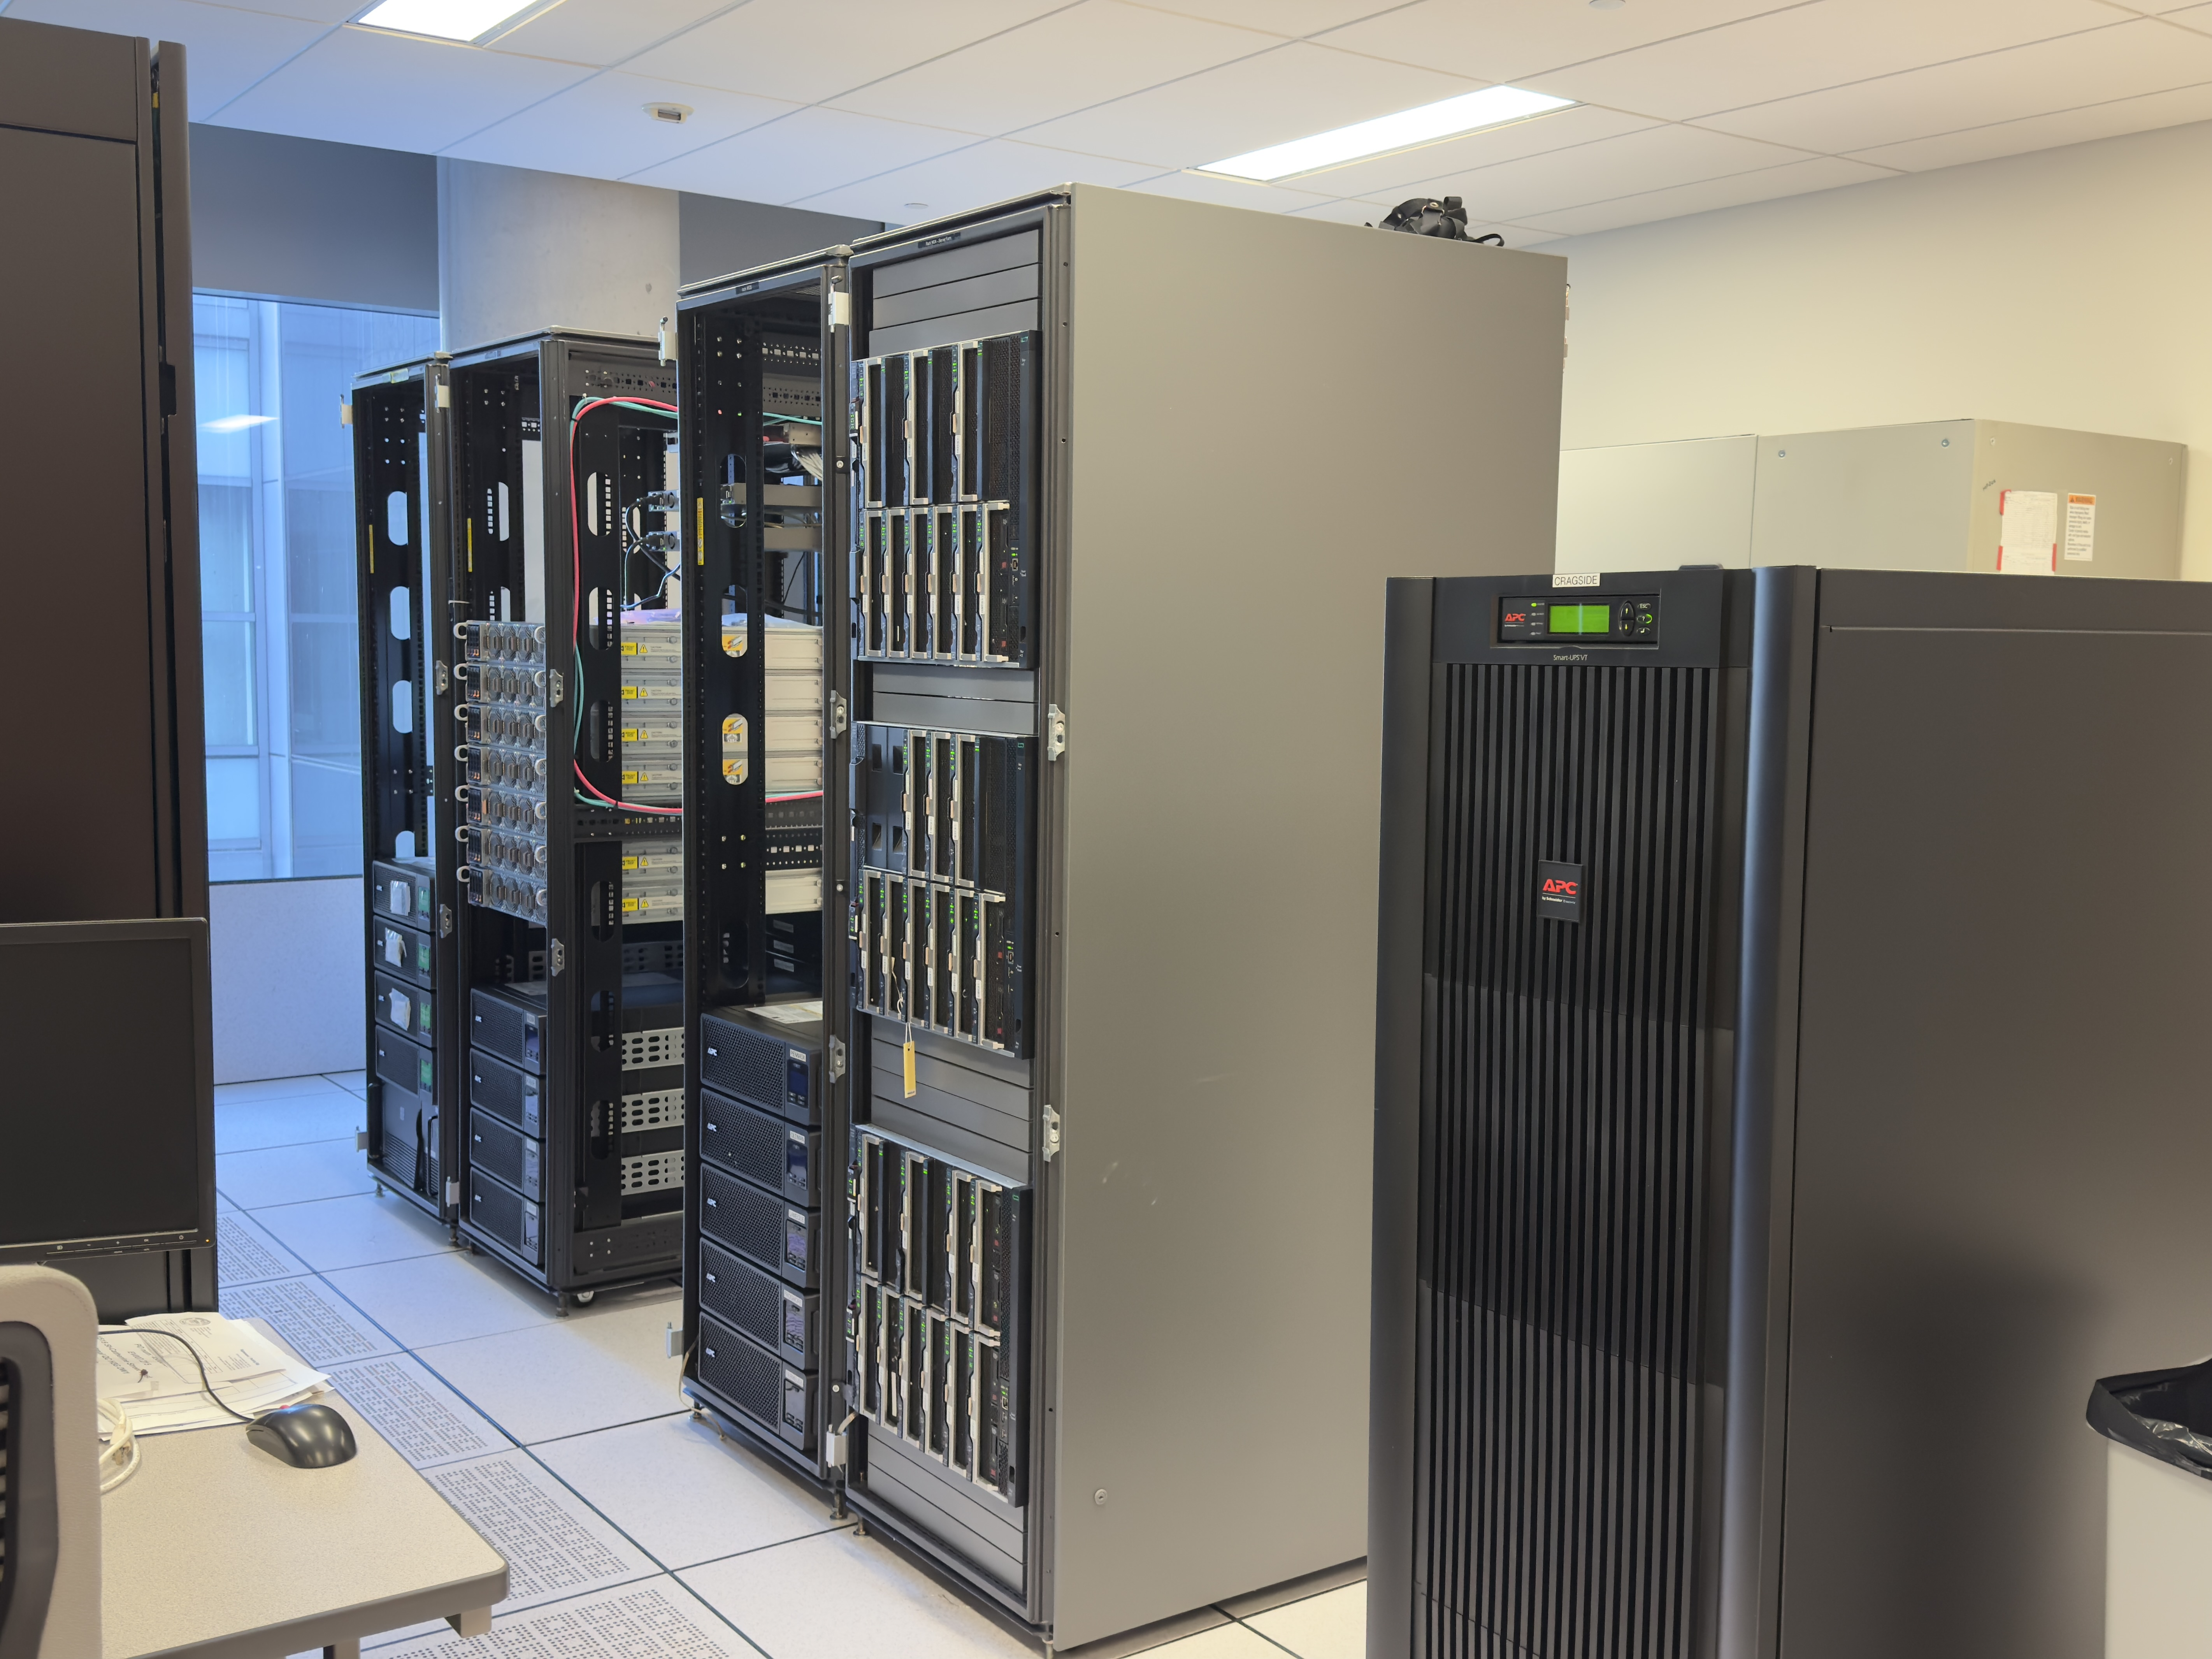
\includegraphics[width=\linewidth]{images/speed2.jpg}
        \caption{Speed Front}
        \label{fig:speed-front}
    \end{minipage}
    \hfill
	% Speed back image
    \begin{minipage}[b]{0.49\columnwidth}
        \centering
        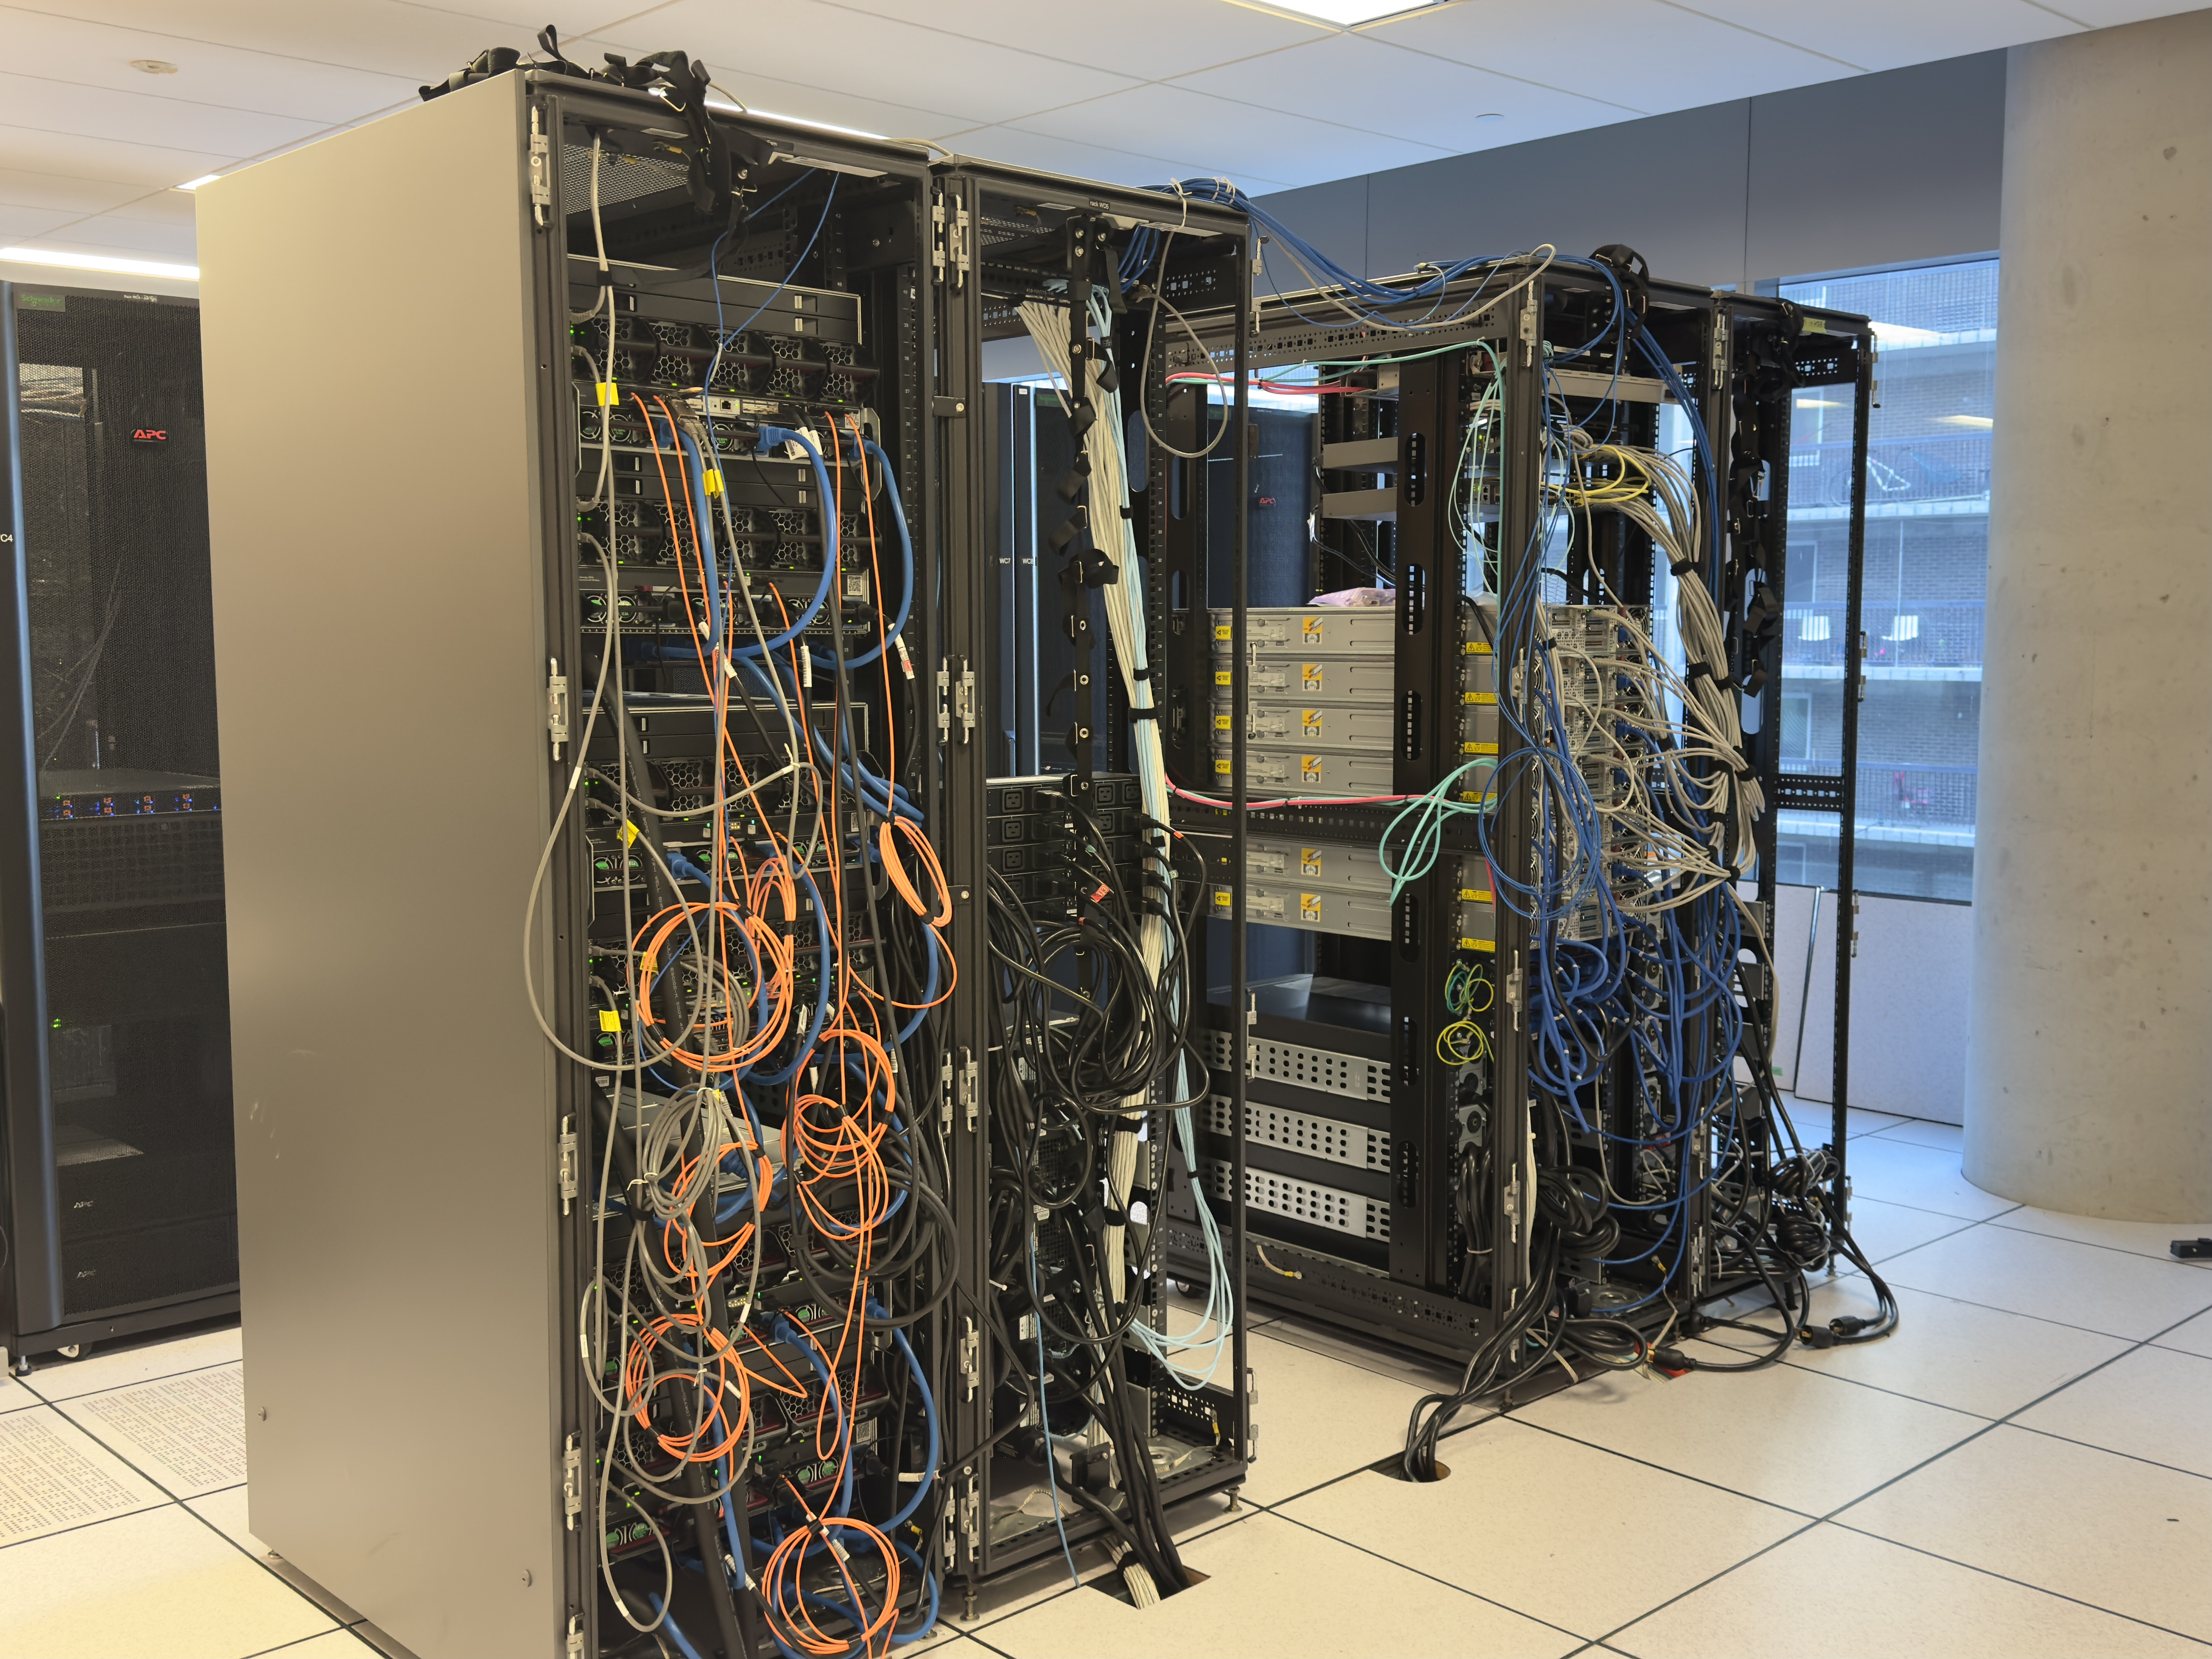
\includegraphics[width=\linewidth]{images/speed1.jpg}
        \caption{Speed Back}
        \label{fig:speed-back}
    \end{minipage}
\end{figure}

\begin{figure}[htbp]
    \centering
    \begin{adjustbox}{center, width=0.2\textwidth}
        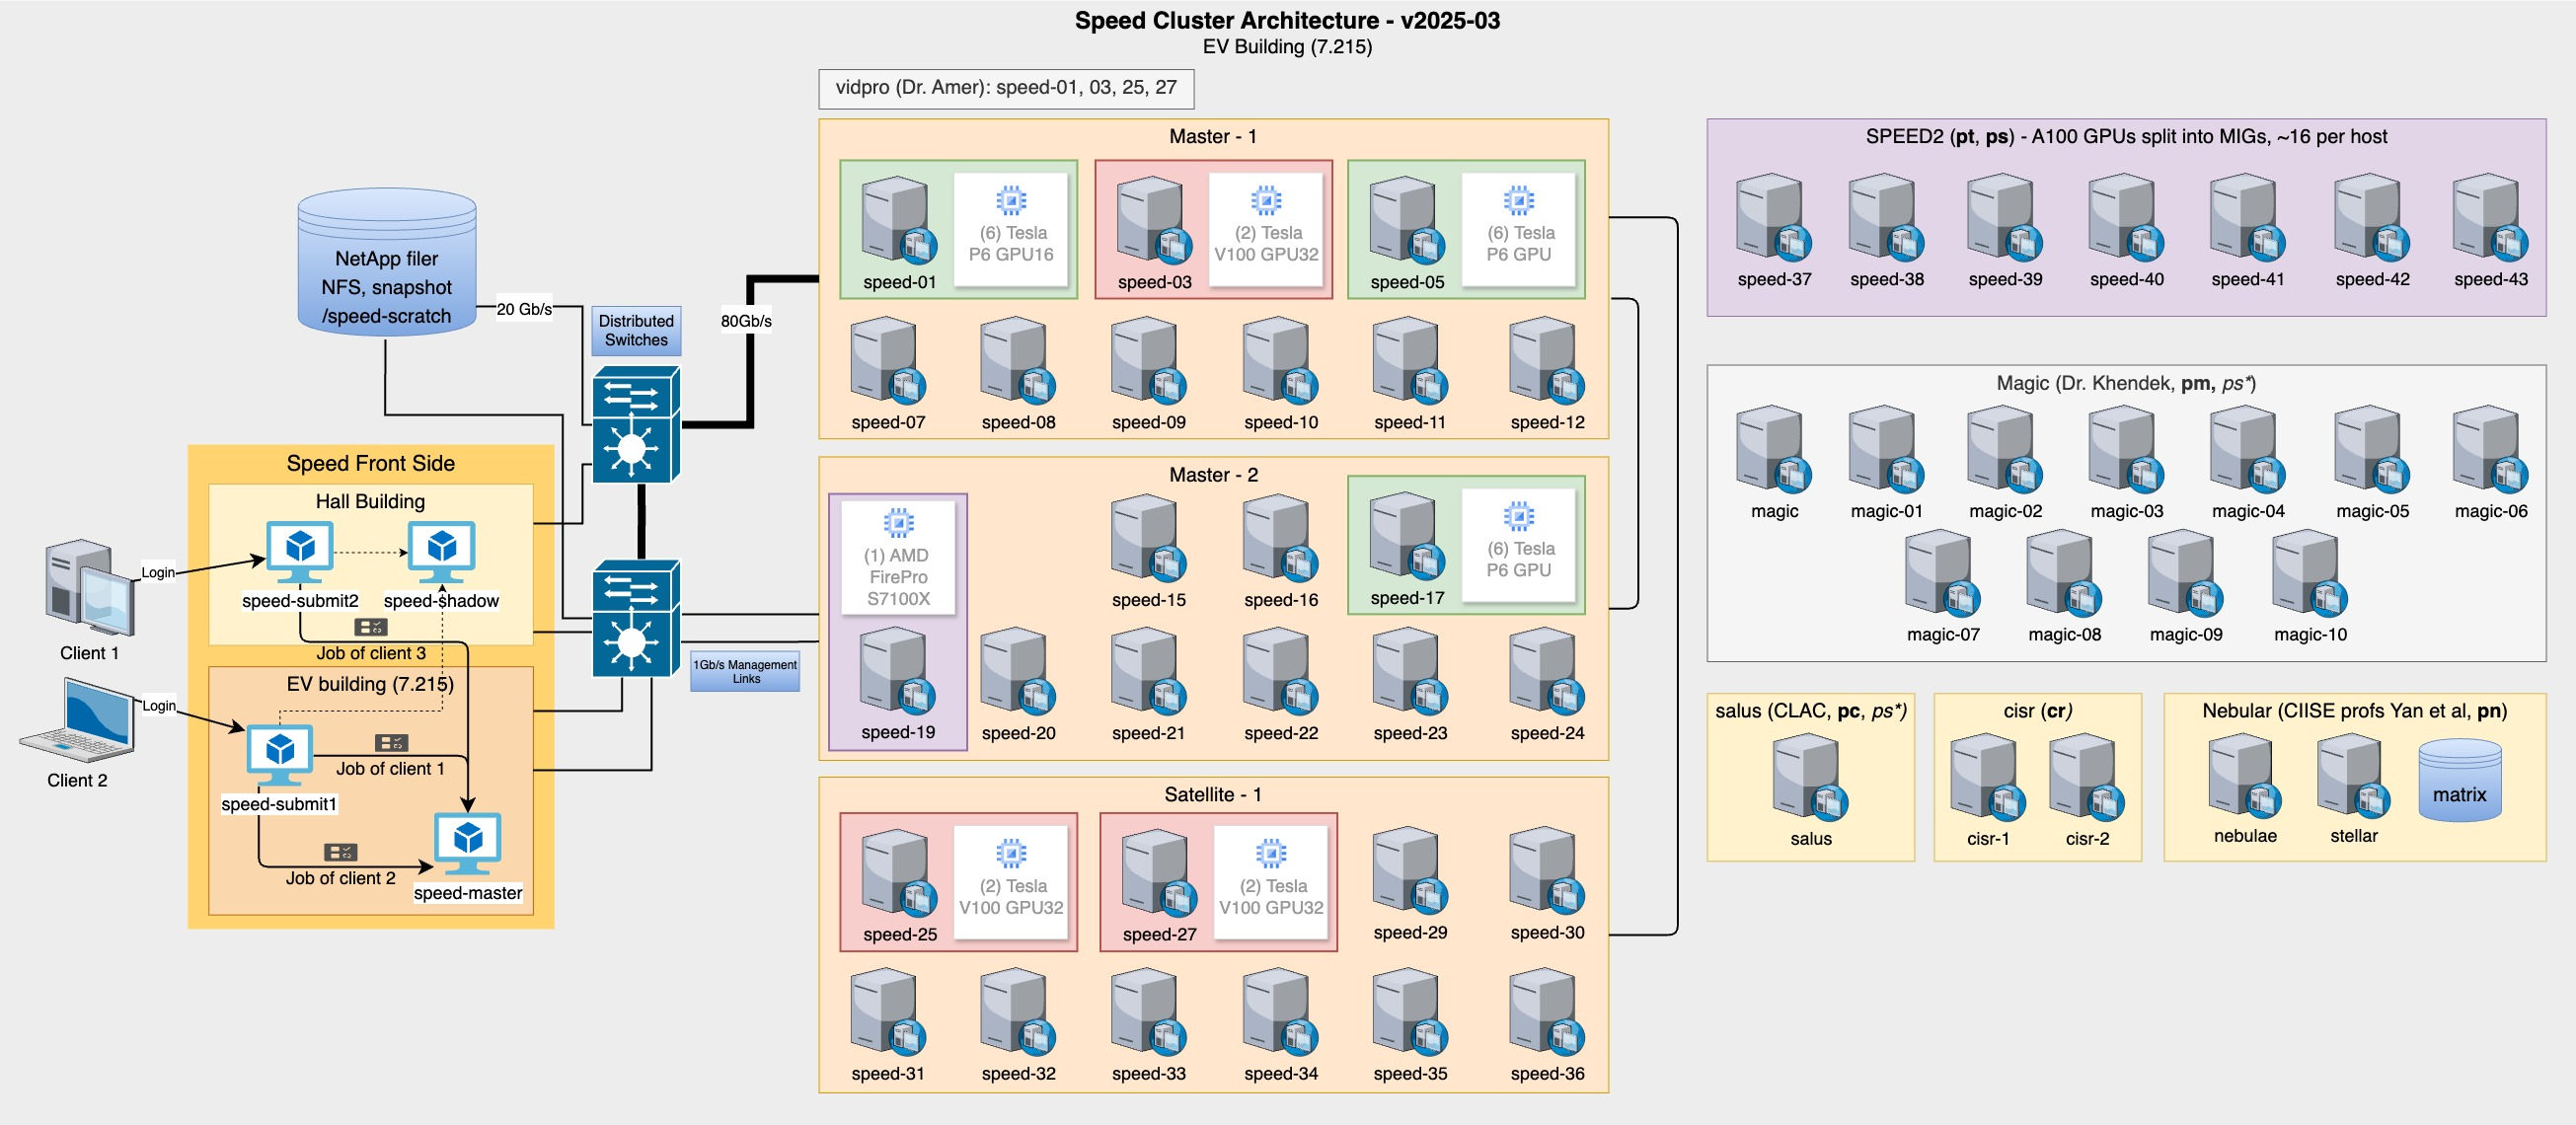
\includegraphics{images/SpeedArchitecture-March 2025.jpg}
    \end{adjustbox}
    \caption{Speed Cluster Hardware Architecture}
    \label{fig:speed-architecture}
\end{figure}

% Slurm architecture image
\begin{figure}[htpb]
	\centering
	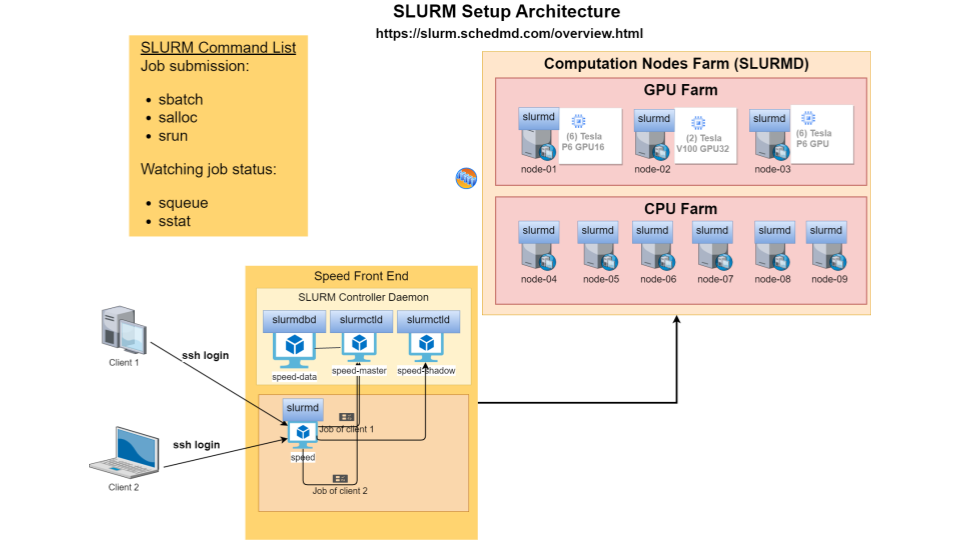
\includegraphics[width=\columnwidth]{images/slurm-arch}
	\caption{Speed SLURM Architecture}
	\label{fig:slurm-arch}
\end{figure}

% 1.5 What Speed Is Ideal For
% -------------------------------------------------------------
\subsection{What Speed Is Ideal For}
\label{sect:speed-is-for}

\begin{itemize}
	\item
	Design, develop, test, and run parallel, batch, and other algorithms and scripts with partial data sets.
	``Speed'' has been optimized for compute jobs that are multi-core aware,
	require a large memory space, or are iteration intensive.

	\item
	Prepare jobs for large clusters such as:
		\begin{itemize}
			\item Digital Research Alliance of Canada (Calcul Quebec and Compute Canada)
			\item Cloud platforms
		\end{itemize}
	\item
	Jobs that are too demanding for a desktop.
	\item
	Single-core batch jobs; multithreaded jobs typically up to 32 cores (i.e., a single machine).
	\item
	Multi-node multi-core jobs (MPI).
	\item
	Anything that can fit into a 500-GB memory space and a \textbf{speed scratch} space of approximately 10~TB. 
	\item
	CPU-based jobs.
	\item
	CUDA GPU jobs.
	\item
	Non-CUDA GPU jobs using OpenCL.
\end{itemize}

% 1.6 What Speed Is Not
% -------------------------------------------------------------
\subsection{What Speed Is Not}
\label{sect:speed-is-not}

\begin{itemize}
	\item Speed is not a web host and does not host websites.
	\item Speed is not meant for Continuous Integration (CI) automation deployments for Ansible or similar tools.
	\item Does not run Kubernetes or other container orchestration software.
	\item Does not run Docker. (\textbf{Note:} Speed does run Singularity and many Docker containers can be converted to
	Singularity containers with a single command. See \xs{sect:singularity-containers}.)
	\item Speed is not for jobs executed outside of the scheduler. (Jobs running outside of the scheduler will be killed and all data lost.)
\end{itemize}

% 1.7 Available Software
% -------------------------------------------------------------
\subsection{Available Software}
\label{sect:available-software}

There are a wide range of open-source and commercial software available and installed on ``Speed.''
This includes Abaqus~\cite{abaqus}, AllenNLP, Anaconda, ANSYS, Bazel,
COMSOL, CPLEX, CUDA, Eclipse, Fluent~\cite{fluent}, Gurobi, MATLAB~\cite{matlab,scholarpedia-matlab},
OMNeT++, OpenCV, OpenFOAM, OpenMPI, OpenPMIx, ParaView, PyTorch, QEMU, R, Rust, and Singularity among others.
Programming environments include various versions of Python, C++/Java compilers, TensorFlow, OpenGL, OpenISS, and {\marf}~\cite{marf}.

In particular, there are over 2200 programs available in \texttt{/encs/bin} and \texttt{/encs/pkg} under Scientific Linux 7 (EL7).
We are building an equivalent array of programs for the EL9 SPEED2 nodes. To see the packages available, run \texttt{ls -al /encs/pkg/} on \texttt{speed.encs}.
See a complete list in \xa{sect:software-list}.

\noindent\textbf{Note:} We do our best to accommodate custom software requests.
Python environments can use user-custom installs from within scratch directory.

% 1.8 Requesting Access
% ------------------------------------------------------------------------------
\subsection{Requesting Access}
\label{sect:access-requests}

After reviewing the ``What Speed is'' (\xs{sect:speed-is-for}) and
``What Speed is Not'' (\xs{sect:speed-is-not}), request access to the ``Speed''
cluster by emailing: \texttt{rt-ex-hpc AT encs.concordia.ca}.

\begin{itemize}
	\item GCS ENCS faculty and staff may request access directly.
	\item GCS students must include the following in their request message:
	\begin{itemize}
		\item GCS ENCS username
		\item Name and email (CC) of the approver -- either a supervisor, course instructor,
		or a department representative (e.g., in the case of undergraduate or M.Eng.\ students it
		can be the Chair, associate chair, a technical officer, or a department administrator) for approval.
		\item Written request from the approver for the GCS ENCS username to be granted access to ``Speed.''
	\end{itemize}
	\item Non-GCS students taking a GCS course will have their GCS ENCS account created automatically, but still need the course instructor's approval to use the service.
	\item Non-GCS faculty and students need to get a ``sponsor'' within GCS, so that a guest GCS ENCS account is created first. A sponsor can be any GCS Faculty member
	you collaborate with. Failing that, request the approval from our Dean's Office;
	via our Associate Deans Drs.~Eddie Hoi Ng or Emad Shihab.
	\item External entities collaborating with GCS Concordia researchers should also go through the Dean's Office for approvals.
\end{itemize}

For detailed instructions, refer to the Concordia
\href{https://www.concordia.ca/ginacody/aits/speed.html}{Computing (HPC) Facility: Speed} webpage.

% Includes:
% 1.1 Citing US
% 1.2 Resources
% 1.3 Team
% 1.4 What Speed Consists of
% 1.5 What Speed Is Ideal For
% 1.6 What Speed Is Not
% 1.7 Available Software
% 1.8 Requesting Access

% ------------------------------------------------------------------------------
%						2 Job Management
% ------------------------------------------------------------------------------
% ------------------------------------------------------------------------------
%						2 Job Management
% ------------------------------------------------------------------------------

We use SLURM as the workload manager. It supports primarily two types of jobs:
batch and interactive. Batch jobs are used to run unattended tasks, whereas,
interactive jobs are are ideal for setting up virtual environments, compilation, and debugging.

\noindent\textbf{Note:} In the following instructions, anything bracketed like, \verb+<>+,
indicates a label/value to be replaced (the entire bracketed term needs replacement).

\noindent Job instructions in a script start with \verb+#SBATCH+ prefix, for example:
\begin{verbatim}
    #SBATCH --mem=100M -t 600 -J <job-name> -A <slurm account>
    #SBATCH -p pg --gpus=1 --mail-type=ALL
\end{verbatim}

For complex compute steps within a script, use \tool{srun}. We recommend using \tool{salloc}
for interactive jobs as it supports multiple steps. However, \tool{srun}
can also be used to start interactive jobs (see \xs{sect:interactive-jobs}).
Common and required job parameters include:

Common and required job parameters include:
%\begin{multicols}{2}
\begin{itemize}
	\item Memory (\option{--mem=<mem>[M|G|T]}),
	\item Partition/Queue (\option{-p <partition>}),
	\item Job name (\option{--job-name=<name>} or \option{-J <name>}),
	\item Wall Clock Limit (\option{-t <min> or -t <days-hh:mm:ss>}),
	\item Event Notification (\option{--mail-type=<events>}),
	\item Email Address (\option{--mail-user=<address>}),
	\item Slurm Account (\option{--account=<account> or -A <account>}),
	\item Tasks Per Node (\option{--tasks-per-node=<count>}),
	\item CPUs Per Task (\option{--cpus-per-task=<count>}),
	\item CPU Count ntasks (\option{-n <count>}).
\end{itemize}
%\end{multicols}

% 2.1 Getting Started
% -------------------------------------------------------------
% 2.1 Getting Started
% -------------------------------------------------------------
\subsection{Getting Started}
\label{sect:getting-started}

Before getting started, please review the ``What Speed is'' (\xs{sect:speed-is-for})
and ``What Speed is Not'' (\xs{sect:speed-is-not}).
Once your GCS ENCS account has been granted access to ``Speed'',
use your GCS ENCS account credentials to create an SSH connection to
\texttt{speed} (an alias for \texttt{speed-submit.encs.concordia.ca}).

All users are expected to have a basic understanding of
Linux and its commonly used commands (see \xa{sect:faqs} for resources).

%  2.1.1 SSH Connection
% -----------------------
\subsubsection{SSH Connections}
\label{sect:ssh-connection}

Requirements to create SSH connection to ``Speed'':
\begin{enumerate}
	\item \textbf{Active GCS ENCS user account:} Ensure you have an active GCS ENCS user account with
	permission to connect to Speed (see \xs{sect:access-requests}).
	\item \textbf{VPN Connection} (for off-campus access): If you are off-campus, you wil need to establish an active connection to Concordia's VPN,
	which requires a Concordia netname.
	\item \textbf{Terminal Emulator for Windows:} Windows systems use a terminal emulator such as PuTTY, Cygwin, or MobaXterm.
	\item \textbf{Terminal for macOS:} macOS systems have a built-in Terminal app or \tool{xterm} that comes with XQuartz.
\end{enumerate}

\noindent To create an SSH connection to Speed, open a terminal window and type the following command, replacing \verb!<ENCSusername>! with your ENCS account's username:
\begin{verbatim}
    ssh <ENCSusername>@speed.encs.concordia.ca
\end{verbatim}

\noindent For detailed instructions on securely connecting to a GCS server, refer to the AITS FAQ:
\href{https://www.concordia.ca/ginacody/aits/support/faq/ssh-to-gcs.html}{How do I securely connect to a GCS server?}

%  2.1.2 Environment Set Up
% --------------------------
\subsubsection{Environment Set Up}
\label{sect:envsetup}
%TO BE DELETED
%% ------------------------------------------------------------------------------
\subsubsection{Environment Set Up}
\label{sect:envsetup}

After creating an SSH connection to ``Speed'', you will need to
make sure the \tool{srun}, \tool{sbatch}, and \tool{salloc}
commands are available to you. 
Type the command name at the linux prompt and press enter.
If the command is not available, e.g.,  (``command not found'') is returned,
you need to make sure your \api{\$PATH} has \texttt{/local/bin} in it.
To view your \api{\$PATH} type \texttt{echo \$PATH} at the linux prompt.
%
%source 
%the ``Altair Grid Engine (AGE)'' scheduler's settings file. 
%Sourcing the settings file will set the environment variables required to 
%execute scheduler commands.
%
%Based on the UNIX shell type, choose one of the following commands to source
%the settings file. 
%
%csh/\tool{tcsh}:
%\begin{verbatim}
%source /local/pkg/uge-8.6.3/root/default/common/settings.csh 
%\end{verbatim}
%
%Bourne shell/\tool{bash}:
%\begin{verbatim}
%. /local/pkg/uge-8.6.3/root/default/common/settings.sh 
%\end{verbatim}
%
%In order to set up the default ENCS bash shell, executing the following command 
%is also required:
%\begin{verbatim}
%printenv ORGANIZATION | grep -qw ENCS || . /encs/Share/bash/profile 
%\end{verbatim}
%
%To verify that you have access to the scheduler commands execute 
%\texttt{qstat -f -u "*"}. If an error is returned, attempt sourcing 
%the settings file again.

The next step is to copy a job template to your home directory and to set up your
cluster-specific storage. Execute the following command from within your
home directory. (To move to your home directory, type \texttt{cd} at the Linux
prompt and press \texttt{Enter}.) 

\begin{verbatim}
cp /home/n/nul-uge/template.sh . && mkdir /speed-scratch/$USER
\end{verbatim}

%\textbf{Tip:} Add the source command to your shell-startup script. 

\textbf{Tip:} the default shell for GCS ENCS users is \tool{tcsh}.
If you would like to use \tool{bash}, please contact 
\texttt{rt-ex-hpc AT encs.concordia.ca}.

%For \textbf{new GCS ENCS Users}, and/or those who don't have a shell-startup script, 
%based on your shell type use one of the following commands to copy a start up script 
%from \texttt{nul-uge}'s home directory to your home directory. (To move to your home
%directory, type \tool{cd} at the Linux prompt and press \texttt{Enter}.)

%csh/\tool{tcsh}:
%\begin{verbatim}
%cp /home/n/nul-uge/.tcshrc . 
%\end{verbatim}

%Bourne shell/\tool{bash}:
%\begin{verbatim}
%cp /home/n/nul-uge/.bashrc . 
%\end{verbatim}

%Users who already have a shell-startup script, can use a text editor, such as
%\tool{vim} or \tool{emacs}, to add the source request to your existing
%shell-startup environment (i.e., to the \file{.tcshrc} file in your home directory). 

%csh/\tool{tcsh}:
%Sample \file{.tcshrc} file:
%\begin{verbatim}
%# Speed environment set up 
%if ($HOSTNAME == speed-submit.encs.concordia.ca) then
   %source /local/pkg/uge-8.6.3/root/default/common/settings.csh
%endif
%\end{verbatim}
%
%Bourne shell/\tool{bash}:
%Sample \file{.bashrc} file:
%\begin{verbatim}
%# Speed environment set up 
%if [ $HOSTNAME = "speed-submit.encs.concordia.ca" ]; then
    %. /local/pkg/uge-8.6.3/root/default/common/settings.sh
    %printenv ORGANIZATION | grep -qw ENCS || . /encs/Share/bash/profile
%fi
%\end{verbatim}

%\noindent
%\textbf{NOTE:} If you have used UGE commands in the past you probably still have these
%lines there; \textbf{they should now be removed}, as they have no use in SLURM:

%csh/\tool{tcsh}:
%Sample \file{.tcshrc} file:
%\begin{verbatim}
%# Speed environment set up 
%if ($HOSTNAME == speed-submit.encs.concordia.ca) then
%   source /local/pkg/uge-8.6.3/root/default/common/settings.csh
%endif
%\end{verbatim}

%Bourne shell/\tool{bash}:
%Sample \file{.bashrc} file:
%\begin{verbatim}
%# Speed environment set up 
%if [ $HOSTNAME = "speed-submit.encs.concordia.ca" ]; then
%    . /local/pkg/uge-8.6.3/root/default/common/settings.sh
%    printenv ORGANIZATION | grep -qw ENCS || . /encs/Share/bash/profile
%fi
%\end{verbatim}

%Note that you will need to either log out and back in, or execute a new shell, 
%for the environment changes in the updated \file{.tcshrc} or \file{.bashrc} file to be applied 
%(\textbf{important}).

%

After creating an SSH connection to Speed, you will need to make sure the \tool{srun}, \tool{sbatch}, and \tool{salloc}
commands are available to you. To check this, type each command at the prompt and press Enter.
If ``command not found'' is returned, you need to make sure your \api{\$PATH} includes \texttt{/local/bin}.
You can check your path by typing:
\begin{verbatim}
    echo $PATH
\end{verbatim}

\noindent The next step is to set up your cluster-specific storage ``speed-scratch'', to do so, execute the following command from within your
home directory.
\begin{verbatim}
    mkdir -p /speed-scratch/$USER && cd /speed-scratch/$USER
\end{verbatim}

\noindent Next, copy a job template to your cluster-specific storage
\begin{itemize}
    \item From Windows drive G: to Speed:\\
    \verb|cp /winhome/<1st letter of $USER>/$USER/<script>.sh /speed-scratch/$USER/|
    \item From Linux drive U: to Speed:\\
    \verb|cp ~/<script>.sh /speed-scratch/$USER/|
\end{itemize}

\noindent \textbf{Tip:} the default shell for GCS ENCS users is \tool{tcsh}.
If you would like to use \tool{bash}, please contact \texttt{rt-ex-hpc AT encs.concordia.ca}.

\noindent \textbf{Note:} If you encounter a ``command not found'' error after logging in to Speed,
your user account may have defunct Grid Engine environment commands.
See \xa{appdx:uge-to-slurm} for instructions on how to resolve this issue.

% includes:
%	2.1.1 SSH Connections
%	2.1.2 Environment Set Up

% 2.2 Job Submission Basics
% -------------------------------------------------------------
% 2.2 Job Submission Basics
% -------------------------------------------------------------
\subsection{Job Submission Basics}
\label{sect:job-submission-basics}

Preparing your job for submission is fairly straightforward.
Start by basing your job script on one of the examples available in the \texttt{src/}
directory of our \href{https://github.com/NAG-DevOps/speed-hpc}{GitHub repository}.
You can clone the repository to get the examples to start with via the command line:

\begin{verbatim}
    git clone --depth=1 https://github.com/NAG-DevOps/speed-hpc.git
    cd speed-hpc/src
\end{verbatim}

\noindent The job script is a shell script that contains directives, module loads, and user scripting.
To quickly run some sample jobs, use the following commands:
\begin{verbatim}
    sbatch -p ps -t 10 env.sh
    sbatch -p ps -t 10 bash.sh
    sbatch -p ps -t 10 manual.sh
    sbatch -p pg -t 10 lambdal-singularity.sh
\end{verbatim}

%  2.2.1 Directives
% -------------------
\subsubsection{Directives}
\label{sect:directives}
% ------------------------------------------------------------------------------
\subsubsection{Directives}
\label{sect:directives}

Directives are comments included at the beginning of a job script that set the shell 
and the options for the job scheduler. 
%
The shebang directive is always the first line of a script. In your job script, 
this directive sets which shell your script's commands will run in. On ``Speed'', 
we recommend that your script use a shell from the \texttt{/encs/bin} directory. 

To use the \texttt{tcsh} shell, start your script with \verb|#!/encs/bin/tcsh|.
%
For \texttt{bash}, start with \verb|#!/encs/bin/bash|.
%
Directives that start with \verb|#SBATCH|, set the options for the cluster's 
Slurm job scheduler. The script template, \texttt{template.sh}, 
provides the essentials:

%\begin{verbatim}
%#$ -N <jobname>
%#$ -cwd
%#$ -m bea
%#$ -pe smp <corecount>
%#$ -l h_vmem=<memory>G
%\end{verbatim}
\begin{verbatim}
#SBATCH --job-name=<jobname>        ## or -J. Give the job a name 
#SBATCH --mail-type=<type>          ## Set type of email notifications
#SBATCH --chdir=<directory>         ## or -D, Set working directory where output files will go 
#SBATCH --nodes=1                   ## or -N, Node count required for the job
#SBATCH --ntasks=1                  ## or -n, Number of tasks to be launched
#SBATCH --cpus-per-task=<corecount> ## or -c, Core count requested, e.g. 8 cores
#SBATCH --mem=<memory>              ## Assign memory for this job, e.g., 32G memory per node 
\end{verbatim}

Replace the following to adjust the job script for your project(s)
\begin{enumerate}
  \item \verb+<jobname>+ with a job name for the job
  \item \verb+<directory>+ with the fullpath to your job's working directory, e.g., where your code,
source files and where the standard output files will be written to. By default, \verb+--chdir+
sets the current directory as the job's working directory 
  \item \verb+<type>+ with the type of e-mail notifications you wish to receive. Valid options are: NONE, BEGIN, END, FAIL, REQUEUE, ALL 
  \item \verb+<corecount>+ with the degree of multithreaded parallelism (i.e., cores) allocated to your job. Up to 32 by default.
  \item \verb+<memory>+ with the amount of memory, in GB, that you want to be allocated per node. Up to 500 depending on the node. 
  NOTE: All jobs MUST set a value for the \verb|--mem| option.
\end{enumerate}

Example with short option equivalents:

\begin{verbatim}
#SBATCH -J tmpdir                   ## Job's name set to 'tmpdir'
#SBATCH --mail-type=ALL             ## Receive all email type notifications
#SBATCH -D ./                       ## Use current directory as working directory
#SBATCH -N 1                        ## Node count required for the job
#SBATCH -n 1                        ## Number of tasks to be launched
#SBATCH -c 8                        ## Request 8 cores
#SBATCH --mem=32G                   ## Allocate 32G memory per node 
\end{verbatim}

%
If you are unsure about memory footprints, err on assigning a generous
memory space to your job, so that it does not get prematurely terminated.
%(the value given to \api{h\_vmem} is a hard memory ceiling).
You can refine
%\api{h\_vmem}
\option{--mem}
values for future jobs by monitoring the size of a job's active
memory space on \texttt{speed-submit} with:

%\begin{verbatim}
%qstat -j <jobID> | grep maxvmem
%\end{verbatim}

\begin{verbatim}
sacct -j <jobID>
sstat -j <jobID>
\end{verbatim}

\noindent
This can be customized to show specific columns:

\begin{verbatim}
sacct -o jobid,maxvmsize,ntasks%7,tresusageouttot%25 -j <jobID>
sstat -o jobid,maxvmsize,ntasks%7,tresusageouttot%25 -j <jobID>
\end{verbatim}

Memory-footprint values are also provided for completed jobs in the final
e-mail notification as ``maxvmsize''.
%
\emph{Jobs that request a low-memory footprint are more likely to load on a busy
cluster.}

Other essential options are \option{--time}, or \verb|-t|, and \option{--account}, or \verb|-A|.
%
\begin{itemize}
\item
\option{--time=<time>} -- is the estimate of wall clock time required for your job to run. 
As preiviously mentioned, the maximum is 7 days for batch and 24 hours for interactive jobs. 
Jobs with a smaller \texttt{time} value will have a higher priority and may result in your job being scheduled sooner. 

\item
\option{--account=<name>} -- specifies which Account, aka project or association, 
that the Speed resources your job uses should be attributed to. When moving from 
GE to SLURM users most users were assigned to Speed's two default accounts 
\texttt{speed1} and \texttt{speed2}. However, users that belong to a particular research
group or project are will have a default Account like the following
\texttt{aits},
\texttt{vidpro},
\texttt{gipsy},
\texttt{ai2},
\texttt{mpackir},
\texttt{cmos}, among others.

\end{itemize}
%TO BE DELETED
%% ------------------------------------------------------------------------------
\subsubsection{Directives}
\label{sect:directives}

Directives are comments included at the beginning of a job script that set the shell 
and the options for the job scheduler. 
%
The shebang directive is always the first line of a script. In your job script, 
this directive sets which shell your script's commands will run in. On ``Speed'', 
we recommend that your script use a shell from the \texttt{/encs/bin} directory. 

To use the \texttt{tcsh} shell, start your script with \verb|#!/encs/bin/tcsh|.
%
For \texttt{bash}, start with \verb|#!/encs/bin/bash|.
%
Directives that start with \verb|#SBATCH|, set the options for the cluster's 
Slurm job scheduler. The script template, \texttt{template.sh}, 
provides the essentials:

%\begin{verbatim}
%#$ -N <jobname>
%#$ -cwd
%#$ -m bea
%#$ -pe smp <corecount>
%#$ -l h_vmem=<memory>G
%\end{verbatim}
\begin{verbatim}
#SBATCH --job-name=<jobname>        ## or -J. Give the job a name 
#SBATCH --mail-type=<type>          ## Set type of email notifications
#SBATCH --chdir=<directory>         ## or -D, Set working directory where output files will go 
#SBATCH --nodes=1                   ## or -N, Node count required for the job
#SBATCH --ntasks=1                  ## or -n, Number of tasks to be launched
#SBATCH --cpus-per-task=<corecount> ## or -c, Core count requested, e.g. 8 cores
#SBATCH --mem=<memory>              ## Assign memory for this job, e.g., 32G memory per node 
\end{verbatim}

Replace the following to adjust the job script for your project(s)
\begin{enumerate}
  \item \verb+<jobname>+ with a job name for the job
  \item \verb+<directory>+ with the fullpath to your job's working directory, e.g., where your code,
source files and where the standard output files will be written to. By default, \verb+--chdir+
sets the current directory as the job's working directory 
  \item \verb+<type>+ with the type of e-mail notifications you wish to receive. Valid options are: NONE, BEGIN, END, FAIL, REQUEUE, ALL 
  \item \verb+<corecount>+ with the degree of multithreaded parallelism (i.e., cores) allocated to your job. Up to 32 by default.
  \item \verb+<memory>+ with the amount of memory, in GB, that you want to be allocated per node. Up to 500 depending on the node. 
  NOTE: All jobs MUST set a value for the \verb|--mem| option.
\end{enumerate}

Example with short option equivalents:

\begin{verbatim}
#SBATCH -J tmpdir                   ## Job's name set to 'tmpdir'
#SBATCH --mail-type=ALL             ## Receive all email type notifications
#SBATCH -D ./                       ## Use current directory as working directory
#SBATCH -N 1                        ## Node count required for the job
#SBATCH -n 1                        ## Number of tasks to be launched
#SBATCH -c 8                        ## Request 8 cores
#SBATCH --mem=32G                   ## Allocate 32G memory per node 
\end{verbatim}

%
If you are unsure about memory footprints, err on assigning a generous
memory space to your job, so that it does not get prematurely terminated.
%(the value given to \api{h\_vmem} is a hard memory ceiling).
You can refine
%\api{h\_vmem}
\option{--mem}
values for future jobs by monitoring the size of a job's active
memory space on \texttt{speed-submit} with:

%\begin{verbatim}
%qstat -j <jobID> | grep maxvmem
%\end{verbatim}

\begin{verbatim}
sacct -j <jobID>
sstat -j <jobID>
\end{verbatim}

\noindent
This can be customized to show specific columns:

\begin{verbatim}
sacct -o jobid,maxvmsize,ntasks%7,tresusageouttot%25 -j <jobID>
sstat -o jobid,maxvmsize,ntasks%7,tresusageouttot%25 -j <jobID>
\end{verbatim}

Memory-footprint values are also provided for completed jobs in the final
e-mail notification as ``maxvmsize''.
%
\emph{Jobs that request a low-memory footprint are more likely to load on a busy
cluster.}

Other essential options are \option{--time}, or \verb|-t|, and \option{--account}, or \verb|-A|.
%
\begin{itemize}
\item
\option{--time=<time>} -- is the estimate of wall clock time required for your job to run. 
As preiviously mentioned, the maximum is 7 days for batch and 24 hours for interactive jobs. 
Jobs with a smaller \texttt{time} value will have a higher priority and may result in your job being scheduled sooner. 

\item
\option{--account=<name>} -- specifies which Account, aka project or association, 
that the Speed resources your job uses should be attributed to. When moving from 
GE to SLURM users most users were assigned to Speed's two default accounts 
\texttt{speed1} and \texttt{speed2}. However, users that belong to a particular research
group or project are will have a default Account like the following
\texttt{aits},
\texttt{vidpro},
\texttt{gipsy},
\texttt{ai2},
\texttt{mpackir},
\texttt{cmos}, among others.

\end{itemize}
%

Directives are comments included at the beginning of a job script that set the shell
and the options for the job scheduler.

The shebang directive is always the first line of a script. In your job script,
this directive sets which shell your script's commands will run in. On ``Speed'',
we recommend that your script use a shell from the \texttt{/encs/bin} directory.

To use \texttt{tcsh} shell, start your script with \verb|#!/encs/bin/tcsh|, for
\texttt{bash}, start with \verb|#!/encs/bin/bash|

Directives that start with \verb|#SBATCH| set the options for the cluster's SLURM job scheduler.
The following provides an example of some essential directives:

\small
\begin{verbatim}
    #SBATCH --job-name=<jobname>        ## or -J. Give the job a name
    #SBATCH --mail-type=<type>          ## set type of email notifications
    #SBATCH --chdir=<directory>         ## or -D, set working directory for the job
    #SBATCH --nodes=1                   ## or -N, node count required for the job
    #SBATCH --ntasks=1                  ## or -n, number of tasks to be launched
    #SBATCH --cpus-per-task=<corecount> ## or -c, core count requested, e.g. 8 cores
    #SBATCH --mem=<memory>              ## assign memory for this job,
                                        ## e.g., 32G memory per node
\end{verbatim}
\normalsize

\noindent Replace the following to adjust the job script for your project(s)
\begin{itemize}
    \item \verb+<jobname>+ with a job name for the job. This name will be displayed in the job queue.
    \item \verb+<directory>+ with the fullpath to your job's working directory, e.g., where your code,
    source files and where the standard output files will be written to.
    By default, \verb+--chdir+ sets the current directory as the job's working directory.
    \item \verb+<type>+ with the type of e-mail notifications you wish to receive.
    Valid options are: NONE, BEGIN, END, FAIL, REQUEUE, ALL.
    \item \verb+<corecount>+ with the degree of multithreaded parallelism (i.e., cores) allocated to your job. Up to 32 by default.
    \item \verb+<memory>+ with the amount of memory, in GB, that you want to be allocated per node. Up to 500 depending on the node.\\
    \textbf{Note}: All jobs MUST set a value for the \option{--mem} option.
\end{itemize}

\noindent Example with short option equivalents:
\small
\begin{verbatim}
    #SBATCH -J myjob              ## Job's name set to 'myjob'
    #SBATCH --mail-type=ALL       ## Receive all email type notifications
    #SBATCH -D ./                 ## Use current directory as working directory
    #SBATCH -N 1                  ## Node count required for the job
    #SBATCH -n 1                  ## Number of tasks to be launched
    #SBATCH -c 8                  ## Request 8 cores
    #SBATCH --mem=32G             ## Allocate 32G memory per node
\end{verbatim}
\normalsize

\noindent \textbf{Tip:} If you are unsure about memory footprints, err on assigning a generous
memory space to your job, so that it does not get prematurely terminated.
You can refine \option{--mem} values for future jobs by monitoring the size of a job's active
memory space on \texttt{speed-submit} with:

\begin{verbatim}
    sacct -j <jobID>
    sstat -j <jobID>
\end{verbatim}

\noindent This can be customized to show specific columns:

\begin{verbatim}
    sacct -o jobid,maxvmsize,ntasks%7,tresusageouttot%25 -j <jobID>
    sstat -o jobid,maxvmsize,ntasks%7,tresusageouttot%25 -j <jobID>
\end{verbatim}

\noindent Memory-footprint efficiency values \tool{seff} are also provided for completed jobs
in the final email notification as ``maxvmsize''.

\emph{Jobs that request a low-memory footprint are more likely to load on a busy cluster.}

\noindent Other essential options are \option{--time}, or \option{-t}, and \option{--account}, or \option{-A}.
\begin{itemize}
    \item \option{--time=<time>} -- is the estimate of wall clock time required for your job to run.
    As previously mentioned, the maximum is 7 days for batch and 24 hours for interactive jobs.
    Jobs with a smaller \texttt{time} value will have a higher priority and may result in your job being scheduled sooner.
    \item \option{--account=<name>} -- specifies which Account, aka project or association,
    that the Speed resources your job uses should be attributed to. When moving from
    GE to SLURM users most users were assigned to Speed's two default accounts
    \texttt{speed1} and \texttt{speed2}. However, users that belong to a particular research
    group or project are will have a default Account like the following
    \texttt{aits},
    \texttt{vidpro},
    \texttt{gipsy},
    \texttt{ai2},
    \texttt{mpackir},
    \texttt{cmos}, among others.
\end{itemize}

%  2.2.2 Module Loads
% -------------------
\subsubsection{Working with Modules}
\label{sect:modules}

After setting the directives in your job script, the next section typically involves loading
the necessary software modules. The \tool{module} command is used to manage the user environment,
make sure to load all the modules your job depends on. You can check available modules with the
module avail command. Loading the correct modules ensures that your environment is properly
set up for execution.

\noindent To list for a particular program (\tool{matlab}, for example):
\small
\begin{verbatim}
    module avail
    module -t avail matlab  ## show the list for a particular program (e.g., matlab)
    module -t avail m       ## show the list for all programs starting with `m'
\end{verbatim}
\normalsize

For example, insert the following in your script to load the \tool{matlab/R2023a} module:
\begin{verbatim}
    module load matlab/R2023a/default
\end{verbatim}

\textbf{Note:} you can remove a module from active use by replacing \option{load} by \option{unload}.

To list loaded modules:
\begin{verbatim}
    module list
\end{verbatim}

To purge all software in your working environment:
\begin{verbatim}
    module purge
\end{verbatim}

%  2.2.3 User Scripting
% -------------------
\subsubsection{User Scripting}
\label{sect:scripting}
%TO BE DELETED
%% ------------------------------------------------------------------------------
\subsubsection{User Scripting}
\label{sect:scripting}

The last part the job script is the scripting that will be executed by the job. 
This part of the job script includes all commands required to set up and 
execute the task your script has been written to do. Any Linux command can be used 
at this step. This section can be a simple call to an executable or a complex 
loop which iterates through a series of commands.

Any compute heavy step is preferably should be prefixed by \tool{srun}
as the best practice.

Every software program has a unique execution framework. It is the responsibility 
of the script's author (e.g., you) to know what is required for the software used 
in your script by reviewing the software's documentation. Regardless of which software
your script calls, your script should be written so that the software knows the 
location of the input and output files as well as the degree of parallelism.
%
% GE:
%Note that the cluster-specific environment variable, \api{NSLOTS}, resolves 
%to the value provided to the scheduler in the \option{-pe smp} option. 

Jobs which touch data-input and data-output files more than once, should make use 
of \api{TMPDIR}, a scheduler-provided working space almost 1~TB in size.
\api{TMPDIR} is created when a job starts, and exists on the local disk of the
compute node executing your job. Using \api{TMPDIR} results in faster I/O operations 
than those to and from shared storage (which is provided over NFS). 

An sample job script using \api{TMPDIR} is available at \texttt{/home/n/nul-uge/templateTMPDIR.sh}: 
the job is instructed to change to \api{\$TMPDIR}, to make the new directory \texttt{input}, to copy data from
%\texttt{\$SGE\_O\_WORKDIR/references/} to \texttt{input/} (\texttt{\$SGE\_O\_WORKDIR} represents the
\texttt{\$SLURM\_SUBMIT\_DIR/references/} to \texttt{input/} (\texttt{\$SLURM\_SUBMIT\_DIR} represents the
current working directory), to make the new directory \texttt{results}, to
execute the program (which takes input from \texttt{\$TMPDIR/input/} and writes
output to \texttt{\$TMPDIR/results/}), and finally to copy the total end results
to an existing directory, \texttt{processed}, that is located in the current
working directory.
% TODO: verify:
TMPDIR only exists for the duration of the job, though,
so it is very important to copy relevant results from it at job's end.

% ------------------------------------------------------------------------------
\subsection{Sample Job Script}

Now, let's look at a basic job script, \file{tcsh.sh} in \xf{fig:tcsh.sh}
(you can copy it from our GitHub page or from \texttt{/home/n/nul-uge}).

\begin{figure}[htpb]
	\lstinputlisting[language=csh,frame=single,basicstyle=\ttfamily]{tcsh.sh}
	\caption{Source code for \file{tcsh.sh}}
	\label{fig:tcsh.sh}
\end{figure}

The first line is the shell declaration (also know as a shebang) and sets the shell to \emph{tcsh}.
%The lines that begin with \texttt{\#\$} are directives for the scheduler.
The lines that begin with \texttt{\#SBATCH} are directives for the scheduler.

\begin{itemize}
	%\item \texttt{-N} sets \emph{qsub-test} as the jobname
	\item \texttt{-J} (or \option{--job-name}) sets \emph{tcsh-test} as the job name
	%\item \texttt{-cwd} tells the scheduler to execute the job from the current working directory
	\item \texttt{--chdir} tells the scheduler to execute the job from the current working directory
	%\item \texttt{-l h\_vmem=1GB} requests and assigns 1GB of memory to the job. CPU jobs \emph{require} the \texttt{-l h\_vmem} option to be set.
	\item \texttt{--mem=1GB} requests and assigns 1GB of memory to the job. 
	Jobs \emph{require} the \texttt{--mem} option to be set either in the script
	or on the command line; \textbf{if it's missing job submission will be rejected.}
\end{itemize}

The script then:

\begin{itemize}
	\item Sleeps on a node for 30 seconds
	\item Uses the \tool{module} command to load the \texttt{gurobi/8.1.0} environment
	\item Prints the list of loaded modules into a file
\end{itemize}

%The scheduler command, \tool{qsub}, is used to submit (non-interactive) jobs. 
The scheduler command, \tool{sbatch}, is used to submit (non-interactive) jobs. 
%From an ssh session on speed-submit, submit this job with \texttt{qsub ./tcsh.sh}.
From an ssh session on speed-submit, submit this job with \texttt{sbatch ./tcsh.sh}.
%You will see, \texttt{"Your job X ("qsub-test") has been submitted"}.
You will see, \texttt{"Submitted batch job 2653"} where $2653$ is a job ID assigned.
%The command, \tool{qstat}, can be used 
The commands, \tool{squeue} and \tool{sinfo} can be used 
%to look at the status of the cluster: \texttt{qstat -f -u "*"}.
to look at the status of the cluster: \texttt{squeue -l}.
You will see something like this: 

%\small
%\begin{verbatim}
%queuename                      qtype resv/used/tot. load_avg arch          states
%---------------------------------------------------------------------------------
%a.q@speed-01.encs.concordia.ca BIP   0/0/32         0.01     lx-amd64
%---------------------------------------------------------------------------------
%a.q@speed-03.encs.concordia.ca BIP   0/0/32         0.01     lx-amd64
%---------------------------------------------------------------------------------
%a.q@speed-25.encs.concordia.ca BIP   0/0/32         0.01     lx-amd64
%---------------------------------------------------------------------------------
%a.q@speed-27.encs.concordia.ca BIP   0/0/32         0.01     lx-amd64
%---------------------------------------------------------------------------------
%g.q@speed-05.encs.concordia.ca BIP   0/0/32         0.02     lx-amd64
     %144   100.00000 qsub-test nul-uge     r     12/03/2018 16:39:30    1 
     %62624 0.09843 case_talle x_yzabc      r     11/09/2021 16:50:09    32
%---------------------------------------------------------------------------------
%g.q@speed-17.encs.concordia.ca BIP   0/0/32         0.01     lx-amd64
%---------------------------------------------------------------------------------
%s.q@speed-07.encs.concordia.ca BIP   0/0/32         0.04     lx-amd64
%---------------------------------------------------------------------------------
%s.q@speed-08.encs.concordia.ca BIP   0/0/32         0.01     lx-amd64
%---------------------------------------------------------------------------------
%s.q@speed-09.encs.concordia.ca BIP   0/0/32         0.01     lx-amd64
%---------------------------------------------------------------------------------
%s.q@speed-10.encs.concordia.ca BIP   0/32/32        32.72    lx-amd64
     %62624 0.09843 case_talle x_yzabc      r     11/09/2021 16:50:09    32
%---------------------------------------------------------------------------------
%s.q@speed-11.encs.concordia.ca BIP   0/32/32        32.08    lx-amd64
     %62679 0.14212 CWLR_DF    a_bcdef      r     11/10/2021 17:25:19    32
%---------------------------------------------------------------------------------
%s.q@speed-12.encs.concordia.ca BIP   0/32/32        32.10    lx-amd64
     %62749 0.09000 CLOUDY     z_abc        r     11/11/2021 21:58:12    32
%---------------------------------------------------------------------------------
%s.q@speed-15.encs.concordia.ca BIP   0/4/32         0.03     lx-amd64
     %62753 82.47478 matlabLDPa b_bpxez      r     11/12/2021 08:49:52     4
%---------------------------------------------------------------------------------
%s.q@speed-16.encs.concordia.ca BIP   0/32/32        32.31    lx-amd64
     %62751 0.09000 CLOUDY     z_abc        r     11/12/2021 06:03:54    32
%---------------------------------------------------------------------------------
%s.q@speed-19.encs.concordia.ca BIP   0/32/32        32.22    lx-amd64
%---------------------------------------------------------------------------------
%...
%---------------------------------------------------------------------------------
%s.q@speed-35.encs.concordia.ca BIP   0/32/32        2.78     lx-amd64
     %62754 7.22952 qlogin-tes a_tiyuu      r     11/12/2021 10:31:06    32
%---------------------------------------------------------------------------------
%s.q@speed-36.encs.concordia.ca BIP   0/0/32         0.03     lx-amd64
%etc.
\small
\begin{verbatim}
[serguei@speed-submit src] % squeue -l
Thu Oct 19 11:38:54 2023
JOBID PARTITION     NAME     USER    STATE       TIME TIME_LIMI  NODES NODELIST(REASON)
 2641        ps interact   b_user  RUNNING   19:16:09 1-00:00:00      1 speed-07
 2652        ps interact   a_user  RUNNING      41:40 1-00:00:00      1 speed-07
 2654        ps tcsh-tes  serguei  RUNNING       0:01 7-00:00:00      1 speed-07
[serguei@speed-submit src] % sinfo
PARTITION AVAIL  TIMELIMIT  NODES  STATE NODELIST
ps*          up 7-00:00:00     14  drain speed-[08-10,12,15-16,20-22,30-32,35-36]
ps*          up 7-00:00:00      1    mix speed-07
ps*          up 7-00:00:00      7   idle speed-[11,19,23-24,29,33-34]
pg           up 1-00:00:00      1  drain speed-17
pg           up 1-00:00:00      3   idle speed-[05,25,27]
pt           up 7-00:00:00      7   idle speed-[37-43]
pa           up 7-00:00:00      4   idle speed-[01,03,25,27]
\end{verbatim}
\normalsize

Remember that you only have 30 seconds before the job is essentially over, so 
if you do not see a similar output, either adjust the sleep time in the 
%script, or execute the \tool{qstat} statement more quickly. The \tool{qstat} 
script, or execute the \tool{sbatch} statement more quickly. The \tool{squeue} 
output listed above shows you that your job is 
running on node \texttt{speed-07}, that it has a job number of 2654,
its time limit of 7 days, etc.
% TODO
%, that it 
%was started at 16:39:30 on 12/03/2018, and that it is a single-core job (the 
%default). 

Once the job finishes, there will be a new file in the directory that the job 
%was started from, with the syntax of, \texttt{"job name".o"job number"}, so 
was started from, with the syntax of, \texttt{slurm-"job id".out}, so 
%in this example the file is, qsub \file{test.o144}. This file represents the 
in this example the file is, \file{slurm-2654.out}. This file represents the 
standard output (and error, if there is any) of the job in question. If you 
look at the contents of your newly created file, you will see that it 
contains the output of the, \texttt{module list} command. 
Important information is often written to this file.
%
%Congratulations on your first job! 

% ------------------------------------------------------------------------------
\subsection{Common Job Management Commands Summary}
\label{sect:job-management-commands}

Here are useful job-management commands: 

\begin{itemize}
%\item
%\texttt{qsub ./<myscript>.sh}: once that your job script is ready,
%on \texttt{speed-submit} you can submit it using this
\item
\texttt{sbatch -A <ACCOUNT> --t <MINUTES> --mem=20G -p <PARTITION> ./<myscript>.sh}: once that your job script is ready,
on \texttt{speed-submit} you can submit it using this

\item
%\texttt{qstat -f -u <ENCSusername>}: you can check the status of your job(s)
\texttt{squeue -u <ENCSusername>}: you can check the status of your job(s)

\item
%\texttt{qstat -f -u "*"}: display cluster status for all users. 
\texttt{squeue}: display cluster status for all users. 
\option{-A} shows per account (e.g., \texttt{vidpro}, \texttt{gipsy},
\texttt{speed1}, \texttt{ai2}, \texttt{aits}, etc.),
\option{-p} per partition (\texttt{ps}, \texttt{pg}, \texttt{pt}, \texttt{pa}),
and others. \texttt{man squeue} for details.

\item
%\texttt{qstat -j [job-ID]}: display job information for [job-ID] (said job may be actually running, or waiting in the queue). 
\texttt{squeue --job [job-ID]}: display job information for [job-ID] (said job may be actually running, or waiting in the queue). 

\item
\texttt{squeue -las}: displays individual job steps (for debugging
easier to see which step failed if you used \tool{srun}).

\item
\verb+watch -n 1 "sinfo -Nel -pps,pt,pg,pa && squeue -la"+: view \tool{sinfo} information and watch the queue for your job(s).

%\item
%\texttt{qdel [job-ID]}: delete job [job-ID]. 
\item
\texttt{scancel [job-ID]}: cancel job [job-ID]. 

%\item
%\texttt{qhold [job-ID]}: hold queued job, [job-ID], from running. 
\item
\texttt{scontrol hold [job-ID]}: hold queued job, [job-ID], from running. 

%\item
%\texttt{qrls [job-ID]}: release held job [job-ID]. 
\item
\texttt{scontrol release [job-ID]}: release held job [job-ID]. 

\item
%\texttt{qacct -j [job-ID]}: get job stats. for completed job [job-ID]. \api{maxvmem} is one of the more useful stats. 
\texttt{sacct -j [job-ID]}: get job stats.
%for completed job [job-ID].
\api{maxvmem} is one of the more useful stats that you can elect to display
as a format option.

\small
\begin{verbatim}
% sacct -j 2654
JobID           JobName  Partition    Account  AllocCPUS      State ExitCode
------------ ---------- ---------- ---------- ---------- ---------- --------
2654          tcsh-test         ps     speed1          1  COMPLETED      0:0
2654.batch        batch                speed1          1  COMPLETED      0:0
2654.extern      extern                speed1          1  COMPLETED      0:0
% sacct -j 2654 -o jobid,user,account,MaxVMSize,Reason%10,TRESUsageOutMax%30
JobID             User    Account  MaxVMSize     Reason        TRESUsageOutMax
------------ --------- ---------- ---------- ---------- ----------------------
2654           serguei     speed1                  None
2654.batch                 speed1    296840K             energy=0,fs/disk=1975
2654.extern                speed1    296312K              energy=0,fs/disk=343
\end{verbatim}
\normalsize

See \texttt{man sacct} or \texttt{sacct -e} for details of the
available formatting options. You can define your preferred
default format in the \api{SACCT\_FORMAT} environment variable
in your \texttt{.cshrc} or \texttt{.bashrc} files.

\end{itemize}


% ------------------------------------------------------------------------------
%\subsection{Advanced \tool{qsub} Options}
\subsection{Advanced \tool{sbatch} Options}
\label{sect:submit-options}
\label{sect:qsub-options}

In addition to the basic \tool{sbatch} options presented earlier, there are a 
few additional options that are generally useful:

\begin{itemize}
\item
%\texttt{-m bea}: requests that the scheduler e-mail you when a job (b)egins;
%(e)nds; (a)borts. Mail is sent to the default address of,
%\texttt{"username@encs.concordia.ca"}, unless a different address is supplied (see, 
%\texttt{-M}). The report sent when a job ends includes job 
%runtime, as well as the maximum memory value hit (\api{maxvmem}). 
\texttt{--mail-type=TYPE}: requests that the scheduler e-mail you when a job changes
state. Where \texttt{TYPE} is \texttt{ALL}, \texttt{BEGIN}, \texttt{END}, or \texttt{FAIL}.
% TODO: verify
Mail is sent to the default address of, \\
\texttt{"<ENCSusername>@encs.concordia.ca"}, which you can consult
via \texttt{webmail.encs} via the VPN, on login.encs via \tool{alpine}
or setup forwarding to @concordia.ca address or offsite,
unless a different address is supplied (see, \texttt{--mail-user}).
% TODO: double-check
The report sent when a job ends includes job 
runtime, as well as the maximum memory value hit (\api{maxvmem}). 

\item
%\texttt{-M email@domain.com}: requests that the scheduler use this e-mail 
%notification address, rather than the default (see, \texttt{-m}). 
\texttt{--mail-user email@domain.com}: requests that the scheduler use this e-mail 
notification address, rather than the default (see, \texttt{--mail-type}). 

\item
%\texttt{-v variable[=value]}: exports an environment variable that can be used by the script.
\texttt{--export=[ALL | NONE | variables]}: exports environment variable(s) that can be used by the script.

\item
%\texttt{-l h\_rt=[hour]:[min]:[sec]}: sets a job runtime of HH:MM:SS. Note 
%that if you give a single number, that represents \emph{seconds}, not hours. 
\texttt{-t [min]} or \texttt{DAYS-HH:MM:SS}: sets a job runtime of min or HH:MM:SS. Note 
that if you give a single number, that represents \emph{minutes}, not hours. 

\item
%\texttt{-hold\_jid [job-ID]}: run this job only when job [job-ID] finishes. Held jobs appear in the queue. 
\texttt{--depend=[state:job-ID]}: run this job only when job [job-ID] finishes. Held jobs appear in the queue. 

\end{itemize}

The many \tool{sbatch} options available are read with, \texttt{man sbatch}. Also 
note that \tool{sbatch} options can be specified during the job-submission 
command, and these \emph{override} existing script options (if present). The 
syntax is, \texttt{sbatch [options] PATHTOSCRIPT}, but unlike in the script, 
the options are specified without the leading \verb+#SBATCH+
(e.g., \texttt{sbatch -J sub-test --chdir=./ --mem=1G ./tcsh.sh}).


% ------------------------------------------------------------------------------
\subsection{Array Jobs}
\label{sect:array-jobs}

Array jobs are those that start a batch job or a parallel job multiple times. 
Each iteration of the job array is called a task and receives a unique job ID.
Only supported for batch jobs; submit time $< 1$ second, compared to repeatedly
submitting the same regular job over and over even from a script.

%To submit an array job, use the \texttt{\-t} option of the \texttt{qsub} 
%command as follows:
To submit an array job, use the \option{--array} option of the \texttt{sbatch} 
command as follows:

%\begin{verbatim}
%qsub -t n[-m[:s]] <batch_script>
%\end{verbatim}
\begin{verbatim}
sbatch --array=n-m[:s]] <batch_script>
\end{verbatim}

\textbf{-t Option Syntax:}
\begin{itemize}
\item
\texttt{n}: indicates the start-id.
\item
\texttt{m}: indicates the max-id.
\item
\texttt{s}: indicates the step size.
\end{itemize}

\textbf{Examples:}
\begin{itemize}
\item
\verb+sbatch --array=1-50000 -N1 -i my_in_%a -o my_out_%a array.sh+: submits a job with 50000 elements,
\%a maps to the task-id between 1 and 50K. 
\item
%\texttt{qsub -t 10 array.sh}: submits a job with 1 task where the task-id is 10. 
\texttt{sbatch --array=10 array.sh}: submits a job with 1 task where the task-id is 10. 
\item
%\texttt{qsub -t 1-10 array.sh}: submits a job with 10 tasks numbered consecutively from 1 to 10.
\texttt{sbatch --array=1-10 array.sh}: submits a job with 10 tasks numbered consecutively from 1 to 10.
\item
%\texttt{qsub -t 3-15:3 array.sh}: submits a jobs with 5 tasks numbered consecutively with step size 3
\texttt{sbatch --array=3-15:3 array.sh}: submits a jobs with 5 tasks numbered consecutively with step size 3
(task-ids 3,6,9,12,15).
\end{itemize}

\textbf{Output files for Array Jobs:}

The default and output and error-files are
%\option{job\_name.[o|e]job\_id} and\\
%\option{job\_name.[o|e]job\_id.task\_id}.
\texttt{slurm-job\_id\_task\_id.out}.
%
This means that Speed creates an output and an error-file for each task 
generated by the array-job as well as one for the super-ordinate array-job. 
To alter this behavior use the \option{-o} and \option{-e} option of
%\tool{qsub}. 
\tool{sbatch}. 

For more details about Array Job options, please review the manual pages for 
%\option{qsub} by executing the following at the command line on speed-submit 
%\tool{man qsub}.
\tool{sbatch} by executing the following at the command line on speed-submit 
\texttt{man sbatch}.
 
% ------------------------------------------------------------------------------
\subsection{Requesting Multiple Cores (i.e., Multithreading Jobs)}

For jobs that can take advantage of multiple machine cores, up to 32 cores
(per job) can be requested in your script with: 

%\begin{verbatim}
%#$ -pe smp [#cores] 
%\end{verbatim}
\begin{verbatim}
#SBATCH -n [#cores for processes] 
\end{verbatim}

or

\begin{verbatim}
#SBATCH -n 1
#SBATCH -c [#cores for threads of a single process]
\end{verbatim}

Both \tool{sbatch} and \tool{salloc} support \option{-n} on the command line,
and it should always be used either in the script or on the command line as the
default $n=1$.
\textbf{Do not request more cores than you think will be useful}, as larger-core
jobs are more difficult to schedule. On the flip side, though, if you 
are going to be running a program that scales out to the maximum single-machine
core count available, please (please) request 32 cores, to avoid node 
oversubscription (i.e., to avoid overloading the CPUs).

\textbf{Important} note about \option{--ntasks} or \option{--ntasks-per-node}
(\option{-n}) talks about processes (usually the ones ran with \tool{srun}).
\option{--cpus-per-task} (\option{-c}) corresponds to threads per process.
Some programs consider them equivalent, some don't. Fluent for example
uses \option{--ntasks-per-node=8} and \option{--cpus-per-task=1},
some just set \option{--cpus-per-task=8} and \option{--ntasks-per-node=1}.
If one of them is not $1$ then some applications need to be told to
use $n*c$ total cores.


Core count associated with a job appears under,
%``states'', in the, \texttt{qstat -f -u "*"}, output.
``AllocCPUS'', in the, \texttt{qacct -j}, output.

\small
\begin{verbatim}
[serguei@speed-submit src] % squeue -l
Thu Oct 19 20:32:32 2023
JOBID PARTITION     NAME     USER    STATE       TIME TIME_LIMI  NODES NODELIST(REASON)
 2652        ps interact   a_user  RUNNING   9:35:18 1-00:00:00      1 speed-07
[serguei@speed-submit src] % sacct -j 2652
JobID           JobName  Partition    Account  AllocCPUS      State ExitCode
------------ ---------- ---------- ---------- ---------- ---------- --------
2652         interacti+         ps     speed1         20    RUNNING      0:0
2652.intera+ interacti+                speed1         20    RUNNING      0:0
2652.extern      extern                speed1         20    RUNNING      0:0
2652.0       gydra_pmi+                speed1         20  COMPLETED      0:0
2652.1       gydra_pmi+                speed1         20  COMPLETED      0:0
2652.2       gydra_pmi+                speed1         20     FAILED      7:0
2652.3       gydra_pmi+                speed1         20     FAILED      7:0
2652.4       gydra_pmi+                speed1         20  COMPLETED      0:0
2652.5       gydra_pmi+                speed1         20  COMPLETED      0:0
2652.6       gydra_pmi+                speed1         20  COMPLETED      0:0
2652.7       gydra_pmi+                speed1         20  COMPLETED      0:0
\end{verbatim}
\normalsize

% ------------------------------------------------------------------------------
\subsection{Interactive Jobs}
\label{sect:interactive-jobs}

Job sessions can be interactive, instead of batch (script) based. Such 
sessions can be useful for testing, debugging, and optimising code and resource 
requirements, conda or python virtual environments setup, or any likewise
preparatory work prior to batch submission.

% ------------------------------------------------------------------------------
\subsubsection{Command Line}

To request an interactive job 
%session, use, \texttt{qlogin [options]}, similarly to a 
%\tool{qsub} command-line job (e.g., \texttt{qlogin -N qlogin-test -l h\_vmem=1G}).
session, use, \texttt{salloc [options]}, similarly to a 
\tool{sbatch} command-line job, e.g.,
%
\begin{verbatim}
salloc -J interactive-test --mem=1G -p ps -n 8
\end{verbatim}
%
%Note that the options that are available for \tool{qsub} are not necessarily
%available for \tool{qlogin}, notably, \texttt{-cwd}, and, \texttt{-v}. 
%
Inside the allocated \tool{salloc} session you can run shell
commands as usual; it is recommended to use \tool{srun} for
the heavy compute steps inside \tool{salloc}.
%
If it is a quick a short job just to compile something, e.g., on
a GPU node you can use an interactive \tool{srun} directly
(note no \tool{srun} can run within \tool{srun}), e.g., a 1 hour
allocation:

For \tool{tcsh}:
\begin{verbatim}
srun --pty -n 8 -p pg --gpus=1 --mem=1Gb -t 60 /encs/bin/tcsh
\end{verbatim}

For \tool{bash}:
\begin{verbatim}
srun --pty -n 8 -p pg --gpus=1 --mem=1Gb -t 60 /encs/bin/bash
\end{verbatim}

% ------------------------------------------------------------------------------
\subsubsection{Graphical Applications}

If you need to run an on-Speed graphical-based UI application (e.g., MALTLAB,
Abaqus CME, etc.), or an IDE (PyCharm, VSCode, Eclipse)
to develop and test your job's code interactively you need to enable
X11-forwarding from your client machine to speed then to the compute node.
To do so:

\begin{enumerate}
\item
you need to run an X server on your client machine, such as,
\begin{itemize}
\item on Windows: MobaXterm with X turned on, or Xming + PuTTY with X11 forwarding, or XOrg under Cygwin
\item on macOS: XQuarz -- use its \tool{xterm} and \texttt{ssh -X}
\item on Linux just use \texttt{ssh -X speed.encs.concordia.ca} 
\end{itemize}

See \url{https://www.concordia.ca/ginacody/aits/support/faq/xserver.html}
for details.

\item
verify your X connection was properly forwarded by printing the \api{DISPLAY} variable:

\verb+echo $DISPLAY+
If it has no output, then your X forwarding is not on and you may need to re-login to Speed.

\item
Use the \option{--x11} with \tool{salloc} or \tool{srun}:

\verb+salloc ... --x11=first ...+

\item
Once landed on a compute node, verify \api{DISPLAY} again.

\item
While running under scheduler, unset \api{XDG\_RUNTIME\_DIR}.

\item
Launch your graphical application:

\texttt{module load} the required version, then
\tool{matlab}, or \tool{abaqus cme}, etc.
\end{enumerate}

Here's an example of starting PyCharm (see \xf{fig:pycharm}), of which we made a sample local installation.
You can make a similar install under your own directory. If using VSCode, it's
currently only supported with the \tool{--no-sandbox} option.

\scriptsize
\begin{verbatim}
bash-3.2$ ssh -X speed (XQuartz xterm, PuTTY or MobaXterm have X11 forwarding too)
serguei@speed's password: 
[serguei@speed-submit ~] % echo $DISPLAY
localhost:14.0
[serguei@speed-submit ~] % srun -p ps --pty --x11=first --mem 4000 -t 0-06:00 /encs/bin/bash
bash-4.4$ echo $DISPLAY
localhost:77.0
bash-4.4$ hostname
speed-01.encs.concordia.ca
bash-4.4$ unset XDG_RUNTIME_DIR
bash-4.4$ /speed-scratch/nag-public/bin/pycharm.sh
\end{verbatim}
\normalsize

\begin{figure}[htpb]
			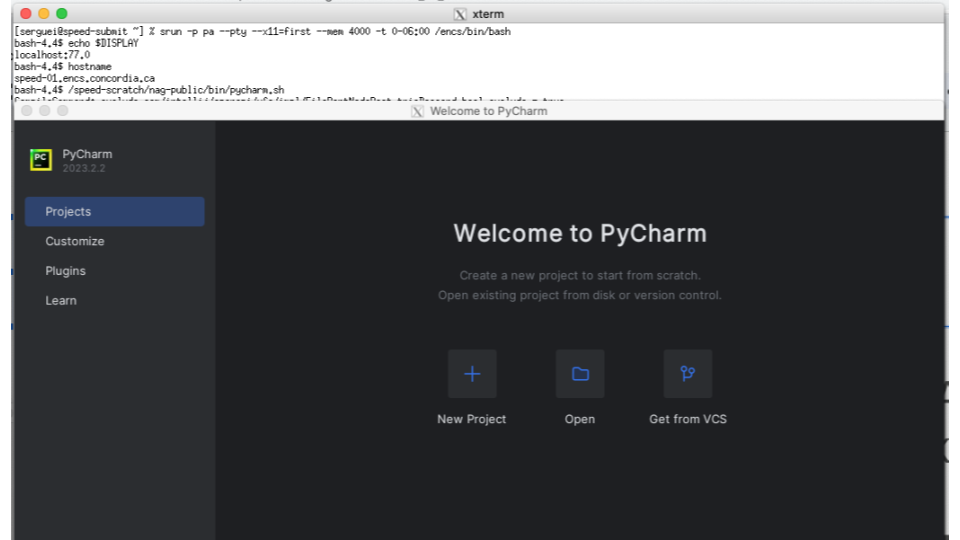
\includegraphics[width=\columnwidth]{images/pycharm}
		\caption{PyCharm Starting up on a Speed Node}
	\label{fig:pycharm}
\end{figure}

% ------------------------------------------------------------------------------
\subsubsection{Jupyter Notebooks}
\label{sect:jupyter}

This is an example of running Jupyter notebooks together with Singularity
(more on Singularity see \xs{sect:singularity-containers}).
Here we are using one of the OpenISS-derived containers (see \xs{sect:openiss-examples} as well).

\begin{enumerate}
\item
Use the \option{--x11} with \tool{salloc} or \tool{srun} as described in the above example

\item
Load Singularity module
\verb+module load singularity/3.10.4/default+

\item
Execute this Singularity command on a single line. It's best to save it in a shell script
that you could call, since it's long.
\scriptsize
\begin{verbatim}
srun singularity exec -B $PWD\:/speed-pwd,/speed-scratch/$USER\:/my-speed-scratch,/nettemp \
 --env SHELL=/bin/bash --nv /speed-scratch/nag-public/openiss-cuda-conda-jupyter.sif \
 /bin/bash -c '/opt/conda/bin/jupyter notebook --no-browser --notebook-dir=/speed-pwd \
 --ip="*" --port=8888 --allow-root'
\end{verbatim}
\normalsize

\item
Create an \tool{ssh} tunnel between your computer and the node (\texttt{speed-XX}) where Jupyter is
running (Using \texttt{speed-submit} as a ``jump server'') (Preferably: PuTTY, see \xf{fig:putty1} and \xf{fig:putty2})
\begin{verbatim}
ssh -L 8888:localhost:8888 speed-XX
\end{verbatim}
Don't close the tunnel.

\item
Open a browser, and copy your Jupyter's token, in the screenshot
example in \xf{fig:jupyter}; each time the token will be different,
as it printed to you in the terminal.

\small
\begin{verbatim}
http://localhost:8888/?token=5a52e6c0c7dfc111008a803e5303371ed0462d3d547ac3fb
\end{verbatim}
\normalsize

\item
Work with your notebook.

\end{enumerate}

\begin{figure}[htbp]
		\centering
		\fbox{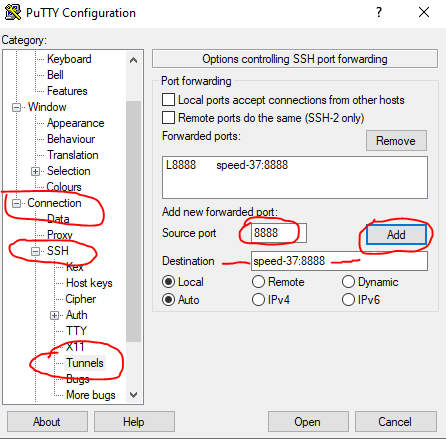
\includegraphics{images/putty1}}
	\caption{SSH tunnel configuration 1}
	\label{fig:putty1}
\end{figure}



\begin{figure}[htbp]
		\centering
		\fbox{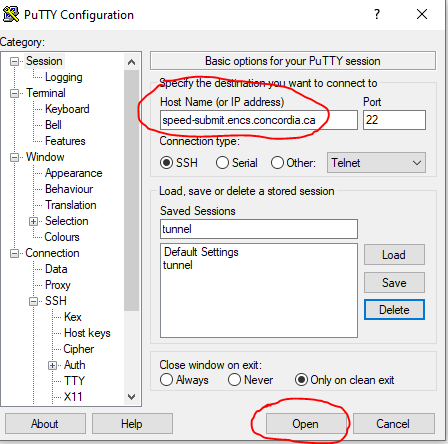
\includegraphics{images/putty2}}
	\caption{SSH tunnel configuration 2}
	\label{fig:putty2}
\end{figure}


\begin{figure}[htbp]
	\centering
	\fbox{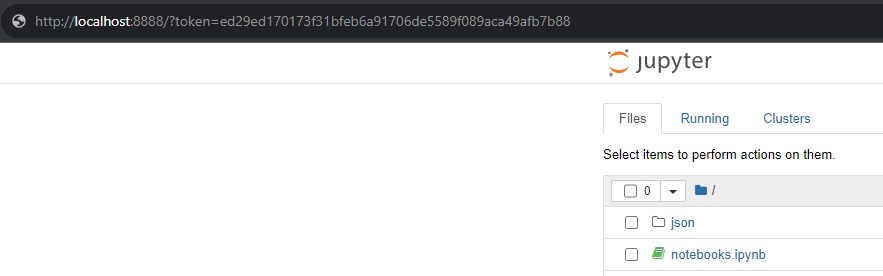
\includegraphics[width=1.00\textwidth]{images/jupyter.png}}
	\caption{Jupyter running on a Speed node}
	\label{fig:jupyter}
\end{figure}

% ------------------------------------------------------------------------------
\subsection{Scheduler Environment Variables}
\label{sect:env-vars}

The scheduler presents a number of environment variables that can be used in 
your jobs. You can invoke \tool{env} or \tool{printenv} in your
job to know what hose are (most begin with the prefix \texttt{SLURM}).
%
Some of the more useful ones are:
%\api{TMPDIR}, \api{SGE\_O\_WORKDIR}, and \api{NSLOTS}:

\begin{itemize}
\item
% TODO: verify temporal existence
\api{\$TMPDIR} -- the path to the job's temporary space on the node. It
\emph{only} exists for the duration of the job, so if data in the temporary space 
are important, they absolutely need to be accessed before the job terminates.

%\item
%\api{\$SGE\_O\_WORKDIR}=the path to the job's working directory (likely an
%NFS-mounted path). If, \texttt{-cwd}, was stipulated, that path is taken; if not, 
%the path defaults to your home directory.
\item
\api{\$SLURM\_SUBMIT\_DIR} -- the path to the job's working directory (likely an
NFS-mounted path). If, \option{--chdir}, was stipulated, that path is taken; if not, 
% TODO: verify if home or current:
the path defaults to your home directory.

% TODO: SLURM does not appear to have this
% SLURM_NTASKS
%\item
%\api{\$NSLOTS}=the number of cores requested for the job. This variable can 
%be used in place of hardcoded thread-request declarations. 

\item
\api{\$SLURM\_JOBID} -- your current jobs ID, useful for some manipulation
and reporting.

\item
\api{\$SLURM\_JOB\_NODELIST}=nodes participating in your job.

\item
\api{\$SLURM\_ARRAY\_TASK\_ID}=for array jobs (see \xs{sect:array-jobs}).

\item
See a more complete list here:

\small
\begin{itemize}
\item
\url{https://slurm.schedmd.com/srun.html#SECTION_INPUT-ENVIRONMENT-VARIABLES}
\item
\url{https://slurm.schedmd.com/srun.html#SECTION_OUTPUT-ENVIRONMENT-VARIABLES}
\end{itemize}
\normalsize

\end{itemize}

\noindent
In \xf{fig:tmpdir.sh} is a sample script, using some of these.

\begin{figure}[htpb]
    \lstinputlisting[language=csh,frame=single,basicstyle=\footnotesize\ttfamily]{tmpdir.sh}
    \caption{Source code for \file{tmpdir.sh}}
	\label{fig:tmpdir.sh}
\end{figure}

%

The final part of the job script involves the commands that will be executed by the job.
This section should include all necessary commands to set up and run the tasks
your script is designed to perform. You can use any Linux command in this section,
ranging from a simple executable call to a complex loop iterating through multiple commands.

\noindent \textbf{Best Practice}: prefix any compute-heavy step with \tool{srun}.
This ensures you gain proper insights on the execution of your job.

\noindent Each software program may have its own execution framework, as it's the script's author (e.g., you)
responsibility to review the software's documentation to understand its requirements.
Your script should be written to clearly specify the location of input and output files and the degree of parallelism needed.

\noindent Jobs that involve multiple interactions with data input and output files, should make use of \api{TMPDIR},
a scheduler-provided workspace nearly 1~TB in size.
\api{TMPDIR} is created on the local disk of the compute node at the start of a job, offering faster I/O operations
compared to shared storage (provided over NFS).

%TO BE DELETED 
% example in /home/n/nul-uge/templateTMPDIR.sh is not accessible.

%An sample job script using \api{TMPDIR} is available at \texttt{/home/n/nul-uge/templateTMPDIR.sh}: 
%the job is instructed to change to \api{\$TMPDIR}, to make the new directory \texttt{input}, to copy data from
%\texttt{\$SLURM\_SUBMIT\_DIR/references/} to \texttt{input/} (\api{\$SLURM\_SUBMIT\_DIR} represents the
%current working directory), to make the new directory \texttt{results}, to
%execute the program (which takes input from \texttt{\$TMPDIR/input/} and writes
%output to \texttt{\$TMPDIR/results/}), and finally to copy the total end results
%to an existing directory, \texttt{processed}, that is located in the current
%working directory.
% TODO: verify:
%\api{TMPDIR} only exists for the duration of the job, though,
%so it is very important to copy relevant results from it at job's end.

% includes:
%	2.2.1 Directives
%	2.2.2 Working with Modules
%	2.2.3 User Scripting

% 2.3 Sample Job Script
% -------------------------------------------------------------
% 2.3 Sample Job Script
% -------------------------------------------------------------
\subsection{Sample Job Script}
\label{sect:sample-job-script}

Here's a basic job script, \file{env.sh} shown in \xf{fig:env.sh}.
You can copy it from our \href{https://github.com/NAG-DevOps/speed-hpc}{GitHub repository}.

\small
\begin{figure}[htpb]
	\lstinputlisting[language=csh,frame=single,basicstyle=\ttfamily\scriptsize]{env.sh}
	\caption{Source code for \file{env.sh}}
	\label{fig:env.sh}
\end{figure}
\normalsize

\noindent The first line is the shell declaration (also know as a shebang) and sets the shell to \emph{tcsh}.
The lines that begin with \texttt{\#SBATCH} are directives for the scheduler.

\begin{itemize}
	\item \option{-J} (or \option{--job-name}) sets \emph{envs} as the job name.
	\item \option{--mail-type} sets the type of notifications.
	\item \option{--chdir} sets the working directory.
	\item \option{--nodes} specifies the number of required nodes.
	\item \option{--ntasks} specifies the number of tasks.
	\item \option{--cpus-per-task} requests 1 cpus.
	\item \option{--mem=} requests memory.

    \textbf{Note:} Jobs require the \option{--mem} option to be set either in the script
	or on the command line; \textbf{job submission will be rejected if it's missing.}
\end{itemize}

\noindent The script then:
\begin{enumerate}
    \item Creates a directory.
	\item Sets TMPDIR to a larger storage.
	\item Prints current date.
	\item Prints env variables.
	\item Prints current date again.
\end{enumerate}

\noindent The scheduler command, \tool{sbatch}, is used to submit (non-interactive) jobs.
From an ssh session on ``speed-submit'', submit this job with
\begin{verbatim}
    sbatch ./env.sh
\end{verbatim}

\noindent You will see, \texttt{Submitted batch job <JOB ID>}.
The commands \tool{squeue} and \tool{sinfo} can be used to look at the queue and the status of the cluster
%\texttt{squeue -l} and \texttt{sinfo -la}.

\small
\begin{verbatim}
[serguei@speed-submit src] % squeue -l
Thu Oct 19 11:38:54 2023
JOBID PARTITION     NAME     USER    STATE       TIME TIME_LIMI  NODES NODELIST(REASON)
 2641        ps interact   b_user   RUNNING   19:16:09 1-00:00:00      1 speed-07
 2652        ps interact   a_user   RUNNING      41:40 1-00:00:00      1 speed-07
 2654        ps envs       serguei  RUNNING       0:01 7-00:00:00      1 speed-07

[serguei@speed-submit src] % sinfo
PARTITION AVAIL  TIMELIMIT  NODES  STATE NODELIST
ps*          up 7-00:00:00      8  drng@ speed-[09-11,15-16,20-21,36]
ps*          up 7-00:00:00      3   drng speed-[38,42-43]
ps*          up 7-00:00:00      2  drain magic-node-[04,08]
ps*          up 7-00:00:00      4    mix magic-node-07,salus,speed-[07,37]
ps*          up 7-00:00:00      7  alloc magic-node-06,speed-[08,12,22-24,29]
ps*          up 7-00:00:00     13   idle magic-node-[05,09-10],speed-[19,30-35,39-41]
pg           up 7-00:00:00      1 drain* speed-05
pg           up 7-00:00:00      2    mix speed-[01,17]
pt           up 7-00:00:00      4   drng speed-[27,38,42-43]
pt           up 7-00:00:00      2    mix speed-[17,37]
pt           up 7-00:00:00      3   idle speed-[39-41]
pa           up 7-00:00:00      1   drng speed-27
pa           up 7-00:00:00      1    mix speed-01
pa           up 7-00:00:00      2   idle speed-[03,25]
cl           up 7-00:00:00      1 drain* speed-05
cl           up 7-00:00:00      4   drng speed-[27,38,42-43]
cl           up 7-00:00:00      3    mix speed-[01,17,37]
cl           up 7-00:00:00      6   idle speed-[03,19,25,39-41]
pc           up 7-00:00:00      1    mix salus
pm           up 7-00:00:00      2  drain magic-node-[04,08]
pm           up 7-00:00:00      1    mix magic-node-07
pm           up 7-00:00:00      1  alloc magic-node-06
pm           up 7-00:00:00      3   idle magic-node-[05,09-10]
pn           up 7-00:00:00      1  down* stellar
pn           up 7-00:00:00      2   idle matrix,nebulae
\end{verbatim}
\normalsize

Once the job finishes, there will be a new file in the directory that the job was started from,
with the syntax of, \texttt{slurm-<job id>.out}. This file represents the standard output
(and error, if there is any) of the job in question.
Important information is often written to this file.
%
%Congratulations on your first job!

% 2.4 Common Job Management Commands
% -------------------------------------------------------------
% 2.4 Common Job Management Commands
% -------------------------------------------------------------
\subsection{Common Job Management Commands}
\label{sect:job-management-commands}

Here is a summary of useful job management commands for handling various aspects of
job submission and monitoring on the Speed cluster:

\begin{itemize}
    \item Submitting a job:
	\begin{verbatim}
		sbatch -A <ACCOUNT> --mem=<MEMORY> -p <PARTITION> ./<myscript>.sh
	\end{verbatim}

	\item Checking your job(s) status:
	\begin{verbatim}
		squeue -u <ENCSusername>
	\end{verbatim}

	\item Displaying cluster status:
	\begin{verbatim}
		squeue
	\end{verbatim}
		\begin{itemize}
			\item Use \option{-A} for per account (e.g., \texttt{-A vidpro}, \texttt{-A aits})
			\item Use \option{-p} for per partition (e.g., \texttt{-p ps}, \texttt{-p pg}, \texttt{-p pt}), etc.
		\end{itemize}

	\item Displaying job information:
	\begin{verbatim}
		squeue --job <job-ID>
	\end{verbatim}

	\item Displaying individual job steps: (to see which step failed if you used \tool{srun})
	\begin{verbatim}
		squeue -las
	\end{verbatim}

	\item Monitoring job and cluster status: (view \tool{sinfo} and watch the queue for your job(s))
	\begin{verbatim}
		watch -n 1 "sinfo -Nel -pps,pt,pg,pa && squeue -la"
	\end{verbatim}

	\item Canceling a job:
	\begin{verbatim}
		scancel <job-ID>
	\end{verbatim}

	\item Holding a job:
	\begin{verbatim}
		scontrol hold <job-ID>
	\end{verbatim}

	\item Releasing a job:
	\begin{verbatim}
		scontrol release <job-ID>
	\end{verbatim}

	\item Getting job statistics: (including useful metrics like ``maxvmem'')
	\begin{verbatim}
		sacct -j <job-ID>
	\end{verbatim}
    \api{maxvmem} is one of the more useful stats that you can elect to display as a format option.

    \small
	\begin{verbatim}
	% sacct -j 2654
	JobID           JobName  Partition    Account  AllocCPUS      State ExitCode
	------------ ---------- ---------- ---------- ---------- ---------- --------
	2654               envs         ps     speed1          1  COMPLETED      0:0
	2654.batch        batch                speed1          1  COMPLETED      0:0
	2654.extern      extern                speed1          1  COMPLETED      0:0
	% sacct -j 2654 -o jobid,user,account,MaxVMSize,Reason%10,TRESUsageOutMax%30
	JobID             User    Account  MaxVMSize     Reason        TRESUsageOutMax
	------------ --------- ---------- ---------- ---------- ----------------------
	2654           serguei     speed1                  None
	2654.batch                 speed1    296840K             energy=0,fs/disk=1975
	2654.extern                speed1    296312K              energy=0,fs/disk=343
	\end{verbatim}
    \normalsize

	See \texttt{man sacct} or \texttt{sacct -e} for details of the available formatting options.
	You can define your preferred default format in the \api{SACCT\_FORMAT} environment variable
	in your \texttt{.cshrc} or \texttt{.bashrc} files.

	\item Displaying job efficiency: (including CPU and memory utilization)
	\begin{verbatim}
	    seff <job-ID>
	\end{verbatim}
    Don't execute it on \texttt{RUNNING} jobs (only on completed/finished jobs), else
	efficiency statistics may be misleading. If you define the following directive in your batch script,
    your GCS ENCS email address will receive an email with \tool{seff}'s output when your job is finished.
	\begin{verbatim}
	    #SBATCH --mail-type=ALL
	\end{verbatim}

	Output example:
	\begin{verbatim}
    Job ID: XXXXX
    Cluster: speed
    User/Group: user1/user1
    State: COMPLETED (exit code 0)
    Nodes: 1
    Cores per node: 4
    CPU Utilized: 00:04:29
    CPU Efficiency: 0.35% of 21:32:20 core-walltime
    Job Wall-clock time: 05:23:05
    Memory Utilized: 2.90 GB
    Memory Efficiency: 2.90% of 100.00 GB
	\end{verbatim}
\end{itemize}

% 2.5 Advanced sbatch Options
% -------------------------------------------------------------
% 2.5 Advanced sbatch Options
% -------------------------------------------------------------
\subsection{Advanced \tool{sbatch} Options}
\label{sect:submit-options}

In addition to the basic sbatch options presented earlier,
there are several advanced options that are generally useful:

\begin{itemize}
	\item E-mail notifications: requests the scheduler to send an email when the job changes state.
	\begin{verbatim}
		--mail-type=<TYPE>
	\end{verbatim}
	\texttt{<TYPE>} can be \texttt{ALL}, \texttt{BEGIN}, \texttt{END}, or \texttt{FAIL}.

	Mail is sent to the default address of \tool{<ENCSusername>@encs.concordia.ca}

	Which you can consult via \url{webmail.encs.concordia.ca} (use VPN from off-campus)
	unless a different address is supplied (see, \option{--mail-user}). The report sent when
    a job ends includes job runtime, as well as the maximum memory value hit (\api{maxvmem}).

    To specify a different email address for notifications rather than the default, use
    \begin{verbatim}
		--mail-user email@domain.com
	\end{verbatim}

	\item Export environment variables used by the script:
	\begin{verbatim}
		--export=ALL
		--export=NONE
		--export=VARIABLES
	\end{verbatim}

	\item Job runtime: sets a job runtime of min or HH:MM:SS. Note that if you give a single number,
	that represents \emph{minutes}, not hours. The set runtime should not exceed
	the default maximums of 24h for interactive jobs and 7 days for batch jobs.
	\begin{verbatim}
		-t <MINUTES> or DAYS-HH:MM:SS
	\end{verbatim}

	\item Job Dependencies: Runs the job only when the specified job \verb|<job-ID>| finishes.
    This is useful for creating job chains where subsequent jobs depend on the completion of previous ones.
	\begin{verbatim}
		--depend=<state:job-ID>
	\end{verbatim}
\end{itemize}

\noindent \textbf{Note:} \tool{sbatch} options can be specified during the job-submission command,
and these \emph{override} existing script options (if present). The syntax is
\begin{verbatim}
	sbatch [options] path/to/script
\end{verbatim}
but unlike in the script, the options are specified without the leading \verb+#SBATCH+
e.g.:
\begin{verbatim}
	sbatch -J sub-test --chdir=./ --mem=1G ./env.sh
\end{verbatim}

% 2.6 Array Jobs
% -------------------------------------------------------------
% 2.6 Array Jobs
% -------------------------------------------------------------
\subsection{Array Jobs}
\label{sect:array-jobs}

Array jobs are those that start a batch job or a parallel job multiple times.
Each iteration of the job array is called a task and receives a unique job ID.
Array jobs are particularly useful for running a large number of similar tasks with slight variations.

To submit an array job (Only supported for batch jobs),
use the \option{--array} option of the \tool{sbatch} command as follows:

\begin{verbatim}
	sbatch --array=n-m[:s] <script>
\end{verbatim}

\textbf{where}
\begin{itemize}
	\item \texttt{n}: indicates the start-id.
	\item \texttt{m}: indicates the max-id.
	\item \texttt{s}: indicates the step size.
\end{itemize}

\textbf{Examples:}
\begin{itemize}
	\item Submit a job with 1 task where the task-id is 10.
	\begin{verbatim}
		sbatch --array=10 array.sh
	\end{verbatim}

	\item Submit a job with 10 tasks numbered consecutively from 1 to 10.
	\begin{verbatim}
		sbatch --array=1-10 array.sh
	\end{verbatim}

	\item Submit a job with 5 tasks numbered consecutively with a step size of 3 (task-ids 3,6,9,12,15).
	\begin{verbatim}
		sbatch --array=3-15:3 array.sh
	\end{verbatim}

	\item Submit a job with 50000 elements, where \%a maps to the task-id between 1 and 50K.
	\begin{verbatim}
		sbatch --array=1-50000 -N1 -i my_in_%a -o my_out_%a array.sh
	\end{verbatim}
\end{itemize}

\textbf{Output files for Array Jobs:}
The default output and error-files are \texttt{slurm-job\_id\_task\_id.out}.
This means that Speed creates an output and an error-file for each task generated by the array-job,
as well as one for the super-ordinate array-job.
To alter this behavior use the \option{-o} and \option{-e} options of \tool{sbatch}.

For more details about Array Job options, please review the manual pages for \tool{sbatch}
by executing the following at the command line on \tool{speed-submit}.
\begin{verbatim}
    man sbatch
\end{verbatim}

% 2.7 Requesting Multiple Cores (i.e., Multithreading Jobs)
% -------------------------------------------------------------
% 2.7 Requesting Multiple Cores (i.e., Multithreading Jobs)
% -------------------------------------------------------------
\subsection{Requesting Multiple Cores (i.e., Multithreading Jobs)}
\label{sect:multicore-jobs}

For jobs that can take advantage of multiple machine cores, you can
request up to 32 cores (per job) in your script using the following options:

\begin{verbatim}
	#SBATCH -n      #cores for processes>
	#SBATCH -n 1
	#SBATCH -c      #cores for threads of a single process
\end{verbatim}

\noindent Both \tool{sbatch} and \tool{salloc} support \option{-n} on the command line,
and it should always be used either in the script or on the command line as the
default $n=1$.

\textbf{Important Considerations}:
\begin{itemize}
	\item Do not request more cores than you think will be useful,
	as larger-core jobs are more difficult to schedule.

	\item If you are running a program that scales out to the maximum single-machine core count available,
    please request 32 cores to avoid node oversubscription (i.e., overloading the CPUs).
\end{itemize}

\textbf{Note:}
\begin{itemize}
    \item\option{--ntasks} or \option{--ntasks-per-node}
    (\option{-n}) refers to processes (usually the ones run with \tool{srun}).
    \item \option{--cpus-per-task} (\option{-c}) corresponds to threads per process.
\end{itemize}

\noindent Some programs consider them equivalent, while others do not.
For example, Fluent uses \option{--ntasks-per-node=8} and \option{--cpus-per-task=1},
whereas others may set \option{--cpus-per-task=8} and \option{--ntasks-per-node=1}.
If one of these is not 1, some applications need to be configured to use \texttt{n * c} total cores.

\noindent Core count associated with a job appears under,``AllocCPUS'', in the, \texttt{sacct -j <job-id>}, output.

\small
\begin{verbatim}
	[serguei@speed-submit src] % squeue -l
	Thu Oct 19 20:32:32 2023
	JOBID PARTITION     NAME     USER    STATE       TIME TIME_LIMI  NODES NODELIST(REASON)
	2652        ps interact   a_user  RUNNING   9:35:18 1-00:00:00      1 speed-07
	[serguei@speed-submit src] % sacct -j 2652
	JobID           JobName  Partition    Account  AllocCPUS      State ExitCode
	------------ ---------- ---------- ---------- ---------- ---------- --------
	2652         interacti+         ps     speed1         20    RUNNING      0:0
	2652.intera+ interacti+                speed1         20    RUNNING      0:0
	2652.extern      extern                speed1         20    RUNNING      0:0
	2652.0       gydra_pmi+                speed1         20  COMPLETED      0:0
	2652.1       gydra_pmi+                speed1         20  COMPLETED      0:0
	2652.2       gydra_pmi+                speed1         20     FAILED      7:0
	2652.3       gydra_pmi+                speed1         20     FAILED      7:0
	2652.4       gydra_pmi+                speed1         20  COMPLETED      0:0
	2652.5       gydra_pmi+                speed1         20  COMPLETED      0:0
	2652.6       gydra_pmi+                speed1         20  COMPLETED      0:0
	2652.7       gydra_pmi+                speed1         20  COMPLETED      0:0
\end{verbatim}
\normalsize

% 2.8 Interactive Jobs
% -------------------------------------------------------------
% 2.8 Interactive Jobs
% -------------------------------------------------------------
\subsection{Interactive Jobs}
\label{sect:interactive-jobs}

Interactive job sessions allow you to interact with the system in real-time.
These sessions are particularly useful for tasks such as testing, debugging, optimizing code,
setting up environments, and other preparatory work before submitting batch jobs.

%  2.8.1 Command Line
% -------------------
\subsubsection{Command Line}
\label{sect:command-line}

To request an interactive job session, use the \texttt{salloc} command with appropriate options.
This is similar to submitting a batch job but allows you to run shell commands interactively
within the allocated resources. For example:
\begin{verbatim}
	salloc -J interactive-test --mem=1G -p ps -n 8
\end{verbatim}

Within the allocated \tool{salloc} session, you can run shell commands as usual.
It is recommended to use \tool{srun} for compute-intensive steps within \tool{salloc}.
If you need a quick, short job just to compile something on a GPU node,
you can use an interactive srun directly. For example, a 1-hour allocation:

\textbf{For tcsh}:
\begin{verbatim}
	srun --pty -n 8 -p pg --gpus=1 --mem=1G -t 60 /encs/bin/tcsh
\end{verbatim}
\textbf{For bash}:
\begin{verbatim}
	srun --pty -n 8 -p pg --gpus=1 --mem=1G -t 60 /encs/bin/bash
\end{verbatim}

% 2.8.2 Graphical Applications
% -----------------------------
\subsubsection{Graphical Applications}
\label{sect:graphical-applications}

To run graphical UI applications (e.g., MALTLAB, Abaqus CME, IDEs like PyCharm, VSCode, Eclipse, etc.) on Speed,
you need to enable X11 forwarding from your client machine Speed then to the compute node.
To do so, follow these steps:
\begin{enumerate}
\item Run an X server on your client machine:
\begin{itemize}
    \item \textbf{Windows:} Use MobaXterm with X turned on, or Xming + PuTTY with X11 forwarding, or XOrg under Cygwin
    \item \textbf{macOS:} Use XQuarz -- use its \tool{xterm} and \texttt{ssh -X}
    \item \textbf{Linux:} Use \texttt{ssh -X speed.encs.concordia.ca}
\end{itemize}
For more details, see \href{https://www.concordia.ca/ginacody/aits/support/faq/xserver.html}{How do I remotely launch X(Graphical) applications?}

\item Verify that X11 forwarding is enabled by printing the \api{DISPLAY} variable:
\begin{verbatim}
    echo $DISPLAY
\end{verbatim}

\item Start an interactive session with X11 forwarding enabled (Use the \option{--x11} with \tool{salloc} or \tool{srun}), for example:
\begin{verbatim}
    salloc -p ps --x11=first --mem=4G -t 0-06:00
\end{verbatim}

\item Once landed on a compute node, verify \api{DISPLAY} again.

\item Set the \api{XDG\_RUNTIME\_DIR} variable to a directory in your \tool{speed-scratch} space:
\begin{verbatim}
    mkdir -p /speed-scratch/$USER/run-dir
    setenv XDG_RUNTIME_DIR /speed-scratch/$USER/run-dir
\end{verbatim}

\item Launch your graphical application:
\begin{verbatim}
    module load matlab/R2023a/default
    matlab
\end{verbatim}
\end{enumerate}

\noindent\textbf{Note:} with X11 forwarding the graphical rendering is happening on your client machine!
That is you are not using GPUs on Speed to render graphics,
instead all graphical information is forwarded from Speed to your desktop or laptop over X11,
which in turn renders it using its own graphics card. Thus, for GPU rendering jobs either keep them
non-interactive or use VirtualGL.

\noindent Here's an example of starting PyCharm (see \xf{fig:pycharm}).
\textbf{Note:} If using VSCode, it's currently only supported with the \tool{--no-sandbox} option.

\textbf{TCSH version:}
\small
\begin{verbatim}
    ssh -X speed (XQuartz xterm, PuTTY or MobaXterm have X11 forwarding too)
    [speed-submit] [/home/c/carlos] > echo $DISPLAY
    localhost:14.0
    [speed-submit] [/home/c/carlos] > cd /speed-scratch/$USER
    [speed-submit] [/speed-scratch/carlos] > echo $DISPLAY
    localhost:13.0
    [speed-submit] [/speed-scratch/carlos] > salloc -pps --x11=first --mem=4Gb -t 0-06:00
    [speed-07] [/speed-scratch/carlos] > echo $DISPLAY
    localhost:42.0
    [speed-07] [/speed-scratch/carlos] > hostname
    speed-07.encs.concordia.ca
    [speed-07] [/speed-scratch/carlos] > setenv XDG_RUNTIME_DIR /speed-scratch/$USER/run-dir
    [speed-07] [/speed-scratch/carlos] > /speed-scratch/nag-public/bin/pycharm.sh
\end{verbatim}
\normalsize

\textbf{BASH version:}
\small
    \begin{verbatim}
    bash-3.2$ ssh -X speed (XQuartz xterm, PuTTY or MobaXterm have X11 forwarding too)
    serguei@speed's password:
    [serguei@speed-submit ~] % echo $DISPLAY
    localhost:14.0
    [serguei@speed-submit ~] % salloc -p ps --x11=first --mem=4Gb -t 0-06:00
    bash-4.4$ echo $DISPLAY
    localhost:77.0
    bash-4.4$ hostname
    speed-01.encs.concordia.ca
    bash-4.4$ export XDG_RUNTIME_DIR=/speed-scratch/$USER/run-dir
    bash-4.4$ /speed-scratch/nag-public/bin/pycharm.sh
\end{verbatim}
\normalsize

\begin{figure}[htpb]
	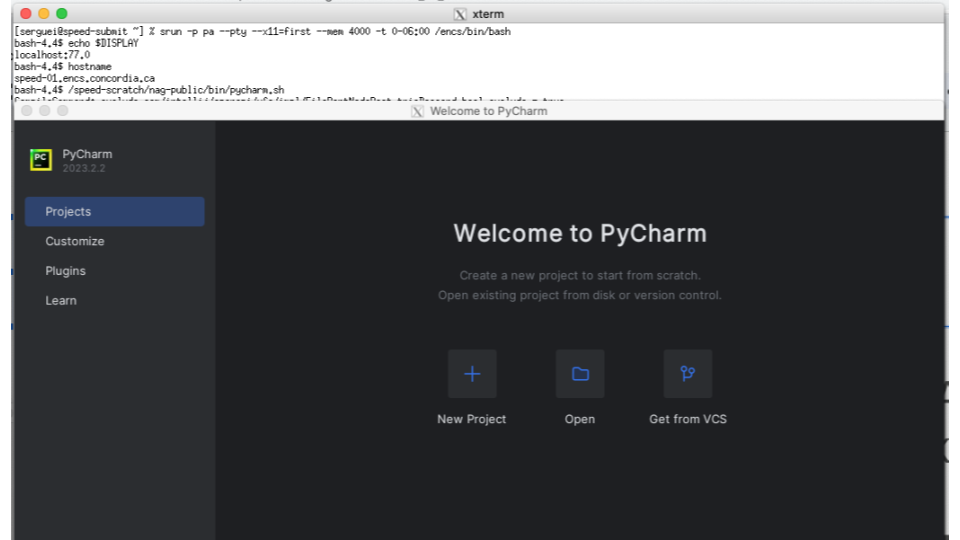
\includegraphics[width=\columnwidth]{images/pycharm}
	\caption{Launching PyCharm on a Speed Node}
	\label{fig:pycharm}
\end{figure}

% 2.8.3 Jupyter Notebooks
% ------------------------
\subsubsection{Jupyter Notebooks}
\label{sect:jupyter-notebooks}

% 2.8.3.1 Jupyter Notebook in Singularity
% ---------------------------------------
\paragraph{Jupyter Notebook in Singularity}
\label{sect:jupyter-singularity}
\noindent To run Jupyter Notebooks using Singularity (more on Singularity see \xs{sect:singularity-containers}),
follow these steps:

\begin{enumerate}
% X11 is not really needed for Jupyter since we tunnel and use a browser
%\item Connect to Speed with X11 forwarding enabled:
\item Connect to Speed, e.g. interactively, using \tool{salloc}
%\item Use the \option{--x11} with \tool{salloc} or \tool{srun} as described in the above example
\item Load Singularity module
    \verb+module load singularity/3.10.4/default+

\item Execute this Singularity command on a single line or save it in a shell script from our
\href{https://github.com/NAG-DevOps/speed-hpc/blob/master/src/jupyter.sh}{GitHub repo}
where you could easily invoke it.

\small
\begin{verbatim}
srun singularity exec -B $PWD\:/speed-pwd,/speed-scratch/$USER\:/my-speed-scratch,/nettemp \
--env SHELL=/bin/bash --nv /speed-scratch/nag-public/openiss-cuda-conda-jupyter.sif \
/bin/bash -c '/opt/conda/bin/jupyter notebook --no-browser --notebook-dir=/speed-pwd \
--ip="*" --port=8888 --allow-root'
\end{verbatim}
\normalsize

\item In a new terminal window, create an \tool{ssh} tunnel between your computer and the node (\texttt{speed-XX}) where Jupyter is
running (using \texttt{speed-submit} as a ``jump server'', see, e.g., in PuTTY, in \xf{fig:putty1} and \xf{fig:putty2})
\small
\begin{verbatim}
    ssh -L 8888:speed-XX:8888 <ENCS-username>@speed-submit.encs.concordia.ca
\end{verbatim}
\normalsize
\textbf{Don't close the tunnel after establishing.}

\item Open a browser, and copy your Jupyter's token (it's printed to you in the terminal)
and paste it in the browser's URL field. In our case, the URL is:
\small
\begin{verbatim}
    http://localhost:8888/?token=5a52e6c0c7dfc111008a803e5303371ed0462d3d547ac3fb
\end{verbatim}
\normalsize

\item Access the Jupyter Notebook interface in your browser.
\end{enumerate}

\begin{figure}[htbp]
	\centering
	\fbox{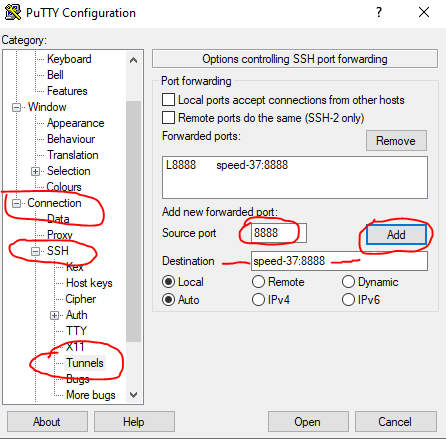
\includegraphics{images/putty1}}
	\caption{SSH tunnel configuration 1}
	\label{fig:putty1}
\end{figure}

\begin{figure}[htbp]
	\centering
	\fbox{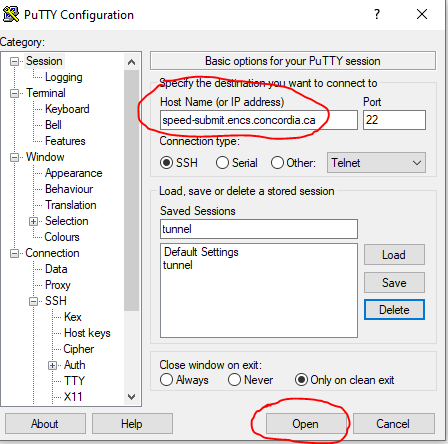
\includegraphics{images/putty2}}
	\caption{SSH tunnel configuration 2}
	\label{fig:putty2}
\end{figure}

\begin{figure}[htbp]
	\centering
	\fbox{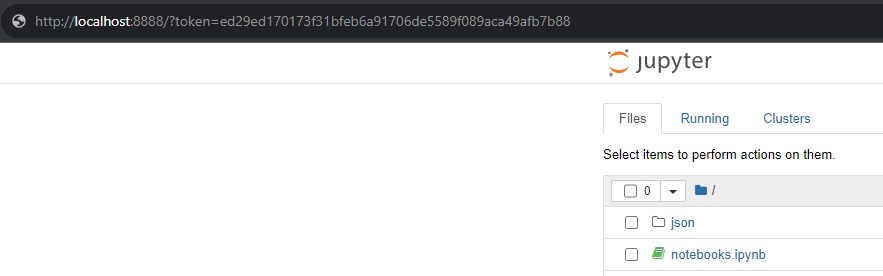
\includegraphics[width=0.9\textwidth]{images/jupyter.png}}
	\caption{Jupyter running on a Speed node}
	\label{fig:jupyter}
\end{figure}

\noindent Another sample is the OpenISS-derived containers with Conda and Jupyter,
see \xs{sect:openiss-examples} for details.

% 2.8.3.2 Jupyter Notebook in Conda
% ----------------------------------
\paragraph{Jupyter Notebook in Conda}
\label{sect:jupyter-conda}

For setting up Jupyter Labs with Conda and Pytorch, follow these steps:

\textbf{Environment preparation:} (only once, takes some time to run to install all required dependencies)
\begin{enumerate}
\item Start an interactive session, and navigate to your \tool{speed-scratch} directory:
\begin{verbatim}
salloc --mem=20G --gpus=1
cd /speed-scratch/$USER
\end{verbatim}

\item Load and initilize the environment
\begin{verbatim}
module load anaconda/2023.03/default
conda init tcsh
source ~/.tcshrc
\end{verbatim}

\item Set up Conda environment by runnung \tool{setup-conda.sh}
(on the compute node salloc brought you to, not on speed-submit)
as shown in \xf{fig:setup_conda.sh}
\begin{verbatim} ./setup_conda.sh \end{verbatim}

\small
\begin{figure}[htpb]
    \lstinputlisting[language=csh,frame=single,basicstyle=\ttfamily\scriptsize]{../../src/jupyterlabs/setup_conda.sh}
    \caption{Source code for \file{setup_conda.sh}}
    \label{fig:setup_conda.sh}
\end{figure}
\normalsize
\end{enumerate}

The script will:
\begin{itemize}
    \item create a Jupyter directory change Jupyter to any name of your choice in the script
    \item set environment variables
    \item create a conda environment named jupyter-env
    \item install JupyterLabs and pytorch
    \item exit the interactive session
\end{itemize}

\textbf{Launching Jupyter Labs instance from \textbf{speed-submit}:}
\begin{enumerate}
    \item Run the \tool{start\_jupyterlab.sh} script each time you need to launch JupyterLab from the submit node
    The script will:
    \begin{itemize}
        \item allocate resources for your job on a compute node
        \item start jupyter server by running \tool{run\_jupyterlab.sh}
        \item print the ssh command that you can use to connect to the compute node runnung the jupyter notebook (this is done in a new terminal)
        \item print the token/link to the jupyter server to paste in a web browser (starting with http://127.0.0.1/...)
    \end{itemize}

    \item Open a browser, and copy your Jupyter's token and paste it in the browser's URL field.
\end{enumerate}


% 2.8.3.3 Jupyter Notebook in Python Virtual Env
% ----------------------------------------------
\paragraph{Jupyter Notebook in Python venv}
\label{sect:jupyter-python}

This is an example of Jupyter Labs running in a Python Virtual environment on Speed.

\textbf{Note:} Use of Python virtual environments is preferred over Conda at Alliance Canada clusters.
If you prefer to make jobs that are more compatible between Speed and Alliance clusters, use Python
\texttt{venv}s. See \url{https://docs.alliancecan.ca/wiki/Anaconda/en}
and \url{https://docs.alliancecan.ca/wiki/JupyterNotebook}.

\begin{itemize}
\item Environment preparation: for the FIRST time only:
\begin{enumerate}
\item Go to your speed-scratch directory: \texttt{cd /speed-scratch/\$USER}
\item Open an interactive session: \texttt{salloc --mem=50G --gpus=1 --constraint=el9}
\item Create a Python \texttt{venv} and install \tool{jupyterlab}+\tool{pytorch}
\small
\begin{verbatim}
module load python/3.11.5/default
setenv TMPDIR /speed-scratch/$USER/tmp
setenv TMP /speed-scratch/$USER/tmp
setenv PIP_CACHE_DIR /speed-scratch/$USER/tmp/cache
python -m venv /speed-scratch/$USER/tmp/jupyter-venv
source /speed-scratch/$USER/tmp/jupyter-venv/bin/activate.csh
pip install jupyterlab
pip3 install torch torchvision torchaudio --index-url https://download.pytorch.org/whl/cu118
exit
\end{verbatim}
\normalsize
\end{enumerate}

\item Running Jupyter, from \textbf{speed-submit}:
\begin{enumerate}
\item Open an interactive session: \texttt{salloc --mem=50G --gpus=1 --constraint=el9}
\small
\begin{verbatim}
cd /speed-scratch/$USER
module load python/3.11.5/default
setenv PIP_CACHE_DIR /speed-scratch/$USER/tmp/cache
source /speed-scratch/$USER/tmp/jupyter-venv/bin/activate.csh
jupyter lab --no-browser --notebook-dir=$PWD --ip="0.0.0.0" --port=8888 --port-retries=50
\end{verbatim}
\normalsize

\item Verify which port the system has assigned to Jupyter: \texttt{http://localhost:XXXX/lab?token=}

\item SSH Tunnel creation: similar to Jupyter in Singularity, see \xs{sect:jupyter-singularity}

\item Open a browser and type: \texttt {localhost:XXXX} (using the port assigned)
\end{enumerate}
\end{itemize}


% 2.8.4 Visual Studio Code
% ------------------------
\subsubsection{Visual Studio Code}
\label{sect:vscode}

This is an example of running VScode, it's similar to Jupyter notebooks, but
it doesn't use containers. \textbf{Note:} this a Web-based version; there exists the local
(workstation)~--~remote (speed-node) client-server version too, but it is for advanced users
and is out of scope here (so no support, use it at your own risk).

\begin{itemize}
\item Environment preparation: for the FIRST time:
\begin{enumerate}
    \item Go to your speed-scratch directory: \texttt{cd /speed-scratch/\$USER}
    \item Create a vscode directory: \texttt{mkdir vscode}
    \item Create another directory: \texttt{mkdir -p /speed-scratch/\$USER/run-user}
\end{enumerate}

\item Running VScode
\begin{enumerate}
    \item Go to your vscode directory:
    \texttt{cd /speed-scratch/\$USER/vscode}
    \item Open interactive session:
    \texttt{salloc --mem=10Gb --constraint=el9}
    \item Set environment variable:
    \texttt{setenv XDG\_RUNTIME\_DIR /speed-scratch/\$USER/run-user}
    \item Run VScode, change the port if needed.
    \scriptsize
    \begin{verbatim}
/speed-scratch/nag-public/code-server-4.22.1/bin/code-server --user-data-dir=$PWD\/projects \
--config=$PWD\/home/.config/code-server/config.yaml --bind-addr="0.0.0.0:8080" $PWD\/projects
    \end{verbatim}
    \normalsize
    \item SSH Tunnel creation: similar to Jupyter, see \xs{sect:jupyter-singularity}
    \item Open a browser and type: \texttt{localhost:8080}
    \item If the browser asks for a password, consult:
    \begin{verbatim}
    cat /speed-scratch/$USER/vscode/home/.config/code-server/config.yaml
    \end{verbatim}
\end{enumerate}
\end{itemize}

\begin{figure}[htbp]
	\centering
	\fbox{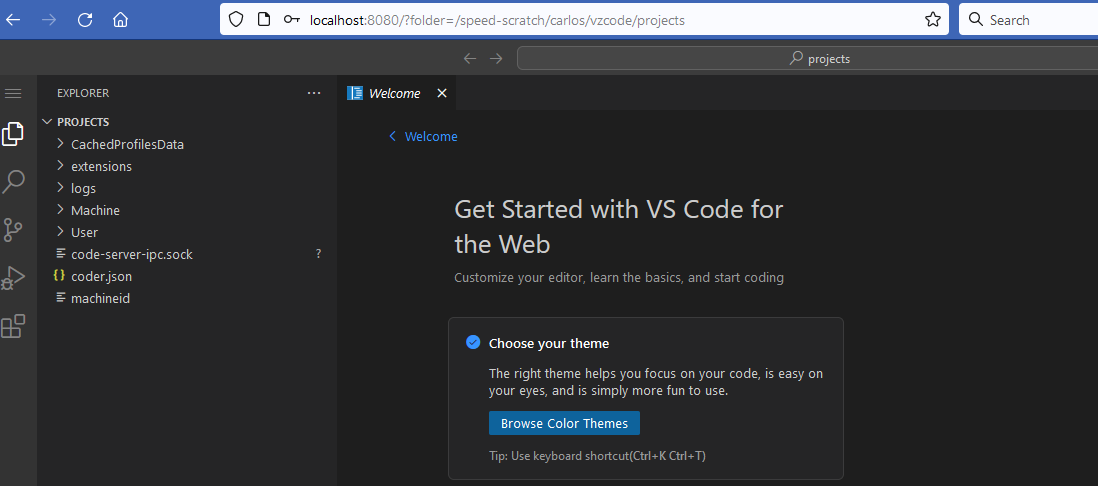
\includegraphics[width=0.9\textwidth]{images/vscode.png}}
	\caption{VScode running on a Speed node}
	\label{fig:vscode}
\end{figure}

% includes:
%	2.8.1 Command Line
%	2.8.2 Graphical Applications
%	2.8.3 Jupyter Notebooks
%		2.8.3.1 Jupyter Notebook in Singularity
%		2.8.3.2 Jupyter Notebook in Conda
%		2.8.3.3 Jupyter Notebook in Python Virtual Env
%	2.8.4 Visual Studio Code

% 2.9 Scheduler Environment Variables
% -------------------------------------------------------------
% 2.9 Scheduler Environment Variables
% -------------------------------------------------------------
\subsection{Scheduler Environment Variables}
\label{sect:env-vars}

The scheduler provides several environment variables that can be useful in your job scripts.
These variables can be accessed within the job using commands like \tool{env} or \tool{printenv}.
Many of these variables start with the prefix \texttt{SLURM}.

\noindent Here are some of the most useful environment variables:

\begin{itemize}
	\item
	\api{\$TMPDIR} (and \api{\$SLURM\_TMPDIR}):
	% TODO: verify temporal existence
	This is the path to the job's temporary space on the node. It \emph{only} exists for the duration of the job.
	If you need the data from this temporary space, ensure you copy it before the job terminates.

	\item
	\api{\$SLURM\_SUBMIT\_DIR}:
	The path to the job's working directory (likely an NFS-mounted path).
	If, \option{--chdir}, was stipulated, that path is taken; if not,
	the path defaults to your home directory.

	\item
	\api{\$SLURM\_JOBID}:
	This variable holds the current job's ID, which is useful for job
	manipulation and reporting within the job's process.

	\item
	\api{\$SLURM\_NTASKS}: the number of cores requested for the job. This variable can
	be used in place of hardcoded thread-request declarations, e.g., for
	Fluent or similar.

	\item
	\api{\$SLURM\_JOB\_NODELIST}:
	This lists the nodes participating in your job.

	\item \api{\$SLURM\_ARRAY\_TASK\_ID}:
	For array jobs, this variable represents the task ID
	(refer to \xs{sect:array-jobs} for more details on array jobs).
\end{itemize}

\noindent For a more comprehensive list of environment variables,
refer to the SLURM documentation for
\href{https://slurm.schedmd.com/srun.html#SECTION_INPUT-ENVIRONMENT-VARIABLES}{Input Environment Variables} and
\href{https://slurm.schedmd.com/srun.html#SECTION_OUTPUT-ENVIRONMENT-VARIABLES}{Output Environment Variables}.

\noindent An example script that utilizes some of these environment variables
is in \xf{fig:tmpdir.sh}.

\begin{figure}[htpb]
    \lstinputlisting[language=csh,frame=single,basicstyle=\scriptsize\ttfamily]{tmpdir.sh}
    \caption{Source code for \file{tmpdir.sh}}
	\label{fig:tmpdir.sh}
\end{figure}

% 2.10 SSH Keys for MPI
% -------------------------------------------------------------
% 2.10 SSH Keys for MPI
% -------------------------------------------------------------
\subsection{SSH Keys for MPI}
\label{sect:ssh-mpi}

Some programs, such as Fluent, utilize MPI (Message Passing Interface) for parallel processing.
MPI requires `passwordless login', which is achieved through SSH keys.
Here are the steps to set up SSH keys for MPI:

\begin{itemize}
	\item Navigate to the \texttt{.ssh} directory
	\begin{verbatim}
	cd ~/.ssh
	\end{verbatim}

	\item Generate a new SSH key pair (Accept the default location and leave the passphrase blank)
	\begin{verbatim}
	ssh-keygen -t ed25519
	\end{verbatim}

	\item Authorize the Public Key:
	\begin{verbatim}
	cat id_ed25519.pub >> authorized_keys
	\end{verbatim}
	If the \texttt{\href{https://www.ssh.com/academy/ssh/authorized-keys-file}{authorized\_keys}} file does not exist, use
	\begin{verbatim}
	cat id_ed25519.pub > authorized_keys
	\end{verbatim}

	\item Set permissions: ensure the correct permissions are set for the `authorized\_keys' file and your home directory
	(most users will already have these permissions by default):
	\begin{verbatim}
	chmod 600 ~/.ssh/authorized_keys
	chmod 700 ~
	\end{verbatim}
\end{itemize}

% 2.11 Creating Virtual Environments
% -------------------------------------------------------------
% 2.11 Creating Virtual Environments
% -------------------------------------------------------------
\subsection{Creating Virtual Environments}
\label{sect:creating-venvs}
\label{sect:environments}
\label{sect:examples-venv}

The following documentation is specific to \textbf{Speed}, other clusters may have their own requirements.
%HPC Facility at the Gina Cody School of Engineering and Computer Science.

Virtual environments are typically created using Conda or Python.
Another option is Singularity (detailed in \xs{sect:singularity-containers}).
These environments are usually created once during an interactive session before
submitting a batch job to the scheduler.

The job script submitted to the scheduler should:
\begin{enumerate}
	\item Activate the virtual environment.
	\item Use the virtual environment.
	\item Deactivate the virtual environment at the end of the job.
\end{enumerate}

%  2.11.1 Anaconda
% -------------------
\subsubsection{Anaconda}
\label{sect:conda-venv}

To create an Anaconda environment, follow these steps:
\begin{enumerate}
	\item Request an interactive session
	\begin{verbatim}
		salloc -p pg --gpus=1
	\end{verbatim}

	\item Load the Anaconda module and create your Anaconda environment in your speed-scratch directory by using
	the \option{--prefix} option (without this o tion, the environment will be created in your home directory by default).
	\begin{verbatim}
		module load anaconda3/2023.03/default
		conda create --prefix /speed-scratch/$USER/myconda
	\end{verbatim}

	\item List environments (to view your conda environment)
	\begin{verbatim}
		conda info --envs
		# conda environments:
		#
		base                  *  /encs/pkg/anaconda3-2023.03/root
                         		 /speed-scratch/a_user/myconda
	\end{verbatim}

	\item Activate the environment
	\begin{verbatim}
		conda activate /speed-scratch/$USER/myconda
	\end{verbatim}

	\item Add \tool{pip} to your environment (this will install \tool{pip} and \tool{pip}'s dependencies,
	including \tool{python}, into the environment.)
	\begin{verbatim}
		conda install pip
	\end{verbatim}
\end{enumerate}

\noindent A consolidated example using Conda:
\begin{verbatim}
    salloc --mem=10G --gpus=1 -p pg -A <slurm account name>
    mkdir -p /speed-scratch/$USER
    cd /speed-scratch/$USER
    module load anaconda3/2023.03/default
    conda create -p /speed-scratch/$USER/pytorch-env
    conda activate /speed-scratch/$USER/pytorch-env
    conda install python=3.11.0
    pip3 install torch torchvision torchaudio --index-url \
    https://download.pytorch.org/whl/cu117
    ....
    conda deactivate
    exit # end the salloc session
\end{verbatim}

\noindent If you encounter \textbf{no space left error} while creating Conda environments, please refer to
\xa{sect:quota-exceeded}.
Likely you forgot \option{--prefix} or environment variables below.

\textbf{Important Note:} \tool{pip} (and \tool{pip3}) are package installers for Python. When you use
\texttt{pip install}, it installs packages from the Python Package Index (PyPI), whereas,
\texttt{conda install} installs packages from Anaconda's repository.

\paragraph{Conda Env without \option{--prefix}}

If you don't want to use the \option{--prefix} option every time you create a new environment and
do not want to use the default home directory, you can create a new directory and set the following
variables to point to the newly created directory, e.g.:
\begin{verbatim}
    mkdir -p /speed-scratch/$USER/conda
    setenv CONDA_ENVS_PATH /speed-scratch/$USER/conda
    setenv CONDA_PKGS_DIRS /speed-scratch/$USER/conda/pkg
\end{verbatim}

\noindent If you want to make these changes permanent, add the variables to your \texttt{.tcshrc}
or \texttt{.bashrc} (depending on the default shell you are using).


% 2.11.2 Python
% -------------------
\subsubsection{Python}
\label{sect:python-venv}

Setting up a Python virtual environment is straightforward.
Here's an example that use a Python virtual environment:

\begin{verbatim}
    salloc --mem=10G --gpus=1 -p pg -A <slurm account name>
    mkdir -p /speed-scratch/$USER
    cd /speed-scratch/$USER
    module load python/3.9.1/default
    mkdir -p /speed-scratch/$USER/tmp
    setenv TMPDIR /speed-scratch/$USER/tmp
    setenv TMP /speed-scratch/$USER/tmp
    python -m venv $TMPDIR/testenv (testenv=name of the virtualEnv)
    source /speed-scratch/$USER/tmp/testenv/bin/activate.csh
    pip install <modules>
    deactivate
    exit
\end{verbatim}

\noindent See, e.g.,
\href{https://github.com/NAG-DevOps/speed-hpc/blob/master/src/gurobi-with-python.sh}
{\texttt{gurobi-with-python.sh}}

\noindent\textbf{Important Note:} our partition \texttt{ps} is used for CPU jobs, while \texttt{pg},
\texttt{pt}, and \texttt{cl} are used for GPU jobs. You do not need to use \option{--gpus}
when preparing environments for CPU jobs.

\noindent\textbf{Note:} Python enviornments are also preferred over Conda
in some clusters, see a note in~\xs{sect:jupyter-python}.

% includes:
%	2.11.1 Anaconda
%		2.11.1.1 Conda Env without --prefix
%	2.11.2 Python

% 2.12 Example Job Script: Fluent
% -------------------------------------------------------------
% 2.12 Example Job Script: Fluent
% -------------------------------------------------------------
% TODO: delete the file
%% -------------- 2.12 Example Job Script: Fluent --------------
% -------------------------------------------------------------
\subsection{Example Job Script: Fluent}

\begin{figure}[htpb]
  \lstinputlisting[language=csh,frame=single,basicstyle=\footnotesize\ttfamily]{fluent.sh}
  \caption{Source code for \texttt{fluent.sh}}
  \label{fig:fluent.sh}
\end{figure}

The job script in \xf{fig:fluent.sh} runs Fluent in parallel over 32 cores. 
Notable aspects of this script include requesting e-mail notifications (\option{--mail-type}), 
defining the parallel environment for Fluent with \option{-t\$SLURM\_NTASKS} and \option{-g-cnf=\$FLUENTNODES}, 
and setting \api{\$TMPDIR} as the in-job location for the ``moment'' \file{rfile.out} file.
The script also copies everything from \api{\$TMPDIR} to a directory in the user's NFS-mounted home after the job completes.
Job progress can be monitored by examining the standard-out file (e.g.,
\texttt{slurm-249.out}), and/or by examining the ``moment'' file in TMPDIR (usually
\texttt{/disk/nobackup/<yourjob>} (it starts with your job-ID)) on the node running
the job. Be cautious with journal-file paths.

% -------------- 2.13 Example Job Script: EfficientDet --------
% -------------------------------------------------------------
\subsection{Example Job: EfficientDet}

The following steps describe how to create an EfficientDet environment on Speed, 
as submitted by a member of Dr. Amer's research group:

\begin{itemize}
  \item Navigate to your \texttt{speed-scratch} directory:
  \begin{verbatim}
	cd /speed-scratch/$USER
  \end{verbatim}
  \item Load Python module
  \begin{verbatim}
	module load python/3.8.3
  \end{verbatim}
  \item Create and activate the virtual environment
  \begin{verbatim}
	python3 -m venv <env_name>
	source <env_name>/bin/activate.csh
  \end{verbatim}
  \item Install DL packages for EfficientDet
  \small
  \begin{verbatim}
	pip install tensorflow==2.7.0
	pip install lxml>=4.6.1
	pip install absl-py>=0.10.0
	pip install matplotlib>=3.0.3
	pip install numpy>=1.19.4
	pip install Pillow>=6.0.0
	pip install PyYAML>=5.1
	pip install six>=1.15.0
	pip install tensorflow-addons>=0.12
	pip install tensorflow-hub>=0.11
	pip install neural-structured-learning>=1.3.1
	pip install tensorflow-model-optimization>=0.5
	pip install Cython>=0.29.13
	pip install git+https://github.com/cocodataset/cocoapi.git#subdirectory=PythonAPI
	\end{verbatim}
  \normalsize
\end{itemize}

% -------------- 2.14 Java Jobs -------------------------------
% -------------------------------------------------------------
\subsection{Java Jobs}
\label{sect:java}

Jobs that call Java have a memory overhead, which needs to be taken 
into account when assigning a value to \option{--mem}. Even the most basic 
Java call, such as \texttt{Java -Xmx1G -version}, will need to have,
\texttt{--mem=5G}, with the 4 GB difference representing the memory overhead. 
\textbf{Note} that this memory overhead grows proportionally with the value of
\texttt{-Xmx}. For example,

\begin{itemize}
  \item When \texttt{-Xmx} has a value of 100G, \option{--mem} has to be at least 106G.
  \item For \texttt{-Xmx} of 200G, \option{--mem} has to be at least 211G.
  \item For \texttt{-Xmx} of 300G, \option{--mem} has to be at least 314G.
\end{itemize}

% TODO: add MARF and GIPSY Java jobs

% -------------- 2.15 Scheduling on the GPU Nodes -------------
% -------------------------------------------------------------
\subsection{Scheduling on the GPU Nodes}
\label{sect:gpu-scheduling}

Speed has various GPU types in various subclusters of its nodes.

\begin{itemize}
	\item \texttt{speed-05} and \texttt{speed-17}:
The primary SPEED1 cluster has two GPU nodes, each with six Tesla (CUDA-compatible) P6
cards. Each card has 2048 cores and 16GB of RAM. Note that the P6
is mainly a single-precision card, so unless you need GPU double precision, 
double-precision calculations will be faster on a CPU node.
	\item \texttt{speed-01}:
This \texttt{vidpro} node (see \xf{fig:speed-architecture-full}, contact Dr.~Maria Amer) is identical
to 05 and 17 in its GPU configuration, but managed by the priority
for the vidpro group, that is a \texttt{pg} job scheduled there
is a subject for preemption.
	\item \texttt{speed-03}, \texttt{speed-25}, \texttt{speed-25}:
These \texttt{vidpro} nodes feature NVIDIA V100 cards with 32GB of RAM.
Like \texttt{speed-01}, the priority is of the vidpro group, who
purchased the nodes, and others' jobs are a subject from preemption
within \texttt{pg}, \texttt{pt}, and \texttt{cl} partitions.
	\item \texttt{speed-37}~--~\texttt{speed-43}:
SPEED2 nodes, the main backbone of the teaching partition \texttt{pt},
have 4x A100 80GB GPUs each, partitioned into average 4x MIGs of 20GB
each, with exceptions.
	\item \texttt{nebulae}:
A member of the Nebular subcluster (contact Dr.~Jun Yan), has 2x 48GB
RTX Ada 6000 cards. This node is in the \texttt{pn} partition.
	\item \texttt{speed-19}:
Has an AMD GPU, Tonga, 16GB of GPU ram.
This node along with the majority of the NVIDIA GPU nodes are in the
\texttt{cl} partition (with restrictions) to run OpenCL, Vulkan,
and HIP jobs.
\end{itemize}

\noindent
Job scripts for the GPU queues differ in that they need these statements,
which attach either a single GPU or more GPUs to the job with the
appropriate partition:
\begin{verbatim}
  #SBATCH --gpus=[1|x]
  #SBATCH -p [pg|pt|cl|pa]
\end{verbatim}
The default max quota for $x$ is 4.

\noindent
Once your job script is ready, submit it to the GPU partition (queue) with:
\begin{verbatim}
  sbatch --mem=<MEMORY> -p pg ./<myscript>.sh
\end{verbatim}
\option{--mem} and \option{-p} can reside in the script.

\noindent
You can query \tool{nvidia-smi} on the node \textbf{running your job} with:
\begin{verbatim}
  ssh <ENCSusername>@speed-[01|03|05|17|25|27|37-43]|nebulae nvidia-smi
\end{verbatim}

\noindent The status of the GPU queues can be queried e.g. with:
\begin{verbatim}
  sinfo -p pg --long --Node
  sinfo -p pt --long --Node
  sinfo -p cl --long --Node
  sinfo -p pa --long --Node
  sinfo -p pn --long --Node
\end{verbatim}

\noindent
You can query \tool{rocm-smi} on the AMD GPU node running your job with:
\begin{verbatim}
  ssh <ENCSusername>@speed-19 rocm-smi
\end{verbatim}

\noindent
\textbf{Important note for TensorFlow and PyTorch users}:
if you are planning to run TensorFlow and/or PyTorch multi-GPU jobs, please
\textbf{do not use} the \api{tf.distribute} and/or \api{torch.nn.DataParallel} functions 
on \textbf{speed-01, speed-05, or speed-17}, as they will crash the compute node (100\% certainty). 
This appears to be a defect in the current hardware architecture.
%
% TODO: Need to link to that example
The workaround is to either manually effect GPU parallelisation (see \xs{sect:multi-node-gpu})
(TensorFlow provides an example on how to do this), or to run on a single GPU,
which is now the default for those nodes.\\

\noindent \textbf{Important}:
Users without permission to use the GPU nodes can submit jobs to the various GPU
partitions, but those jobs will hang and never run.
Their availability can be seen with:
%
\small
\begin{verbatim}
[serguei@speed-submit src] % sinfo -p pg --long --Node
Thu Oct 19 22:31:04 2023
NODELIST   NODES PARTITION       STATE CPUS    S:C:T MEMORY TMP_DISK WEIGHT AVAIL_FE REASON
speed-05       1        pg        idle 32     2:16:1 515490        0      1    gpu16 none
speed-17       1        pg     drained 32     2:16:1 515490        0      1    gpu16 UGE
speed-25       1        pg        idle 32     2:16:1 257458        0      1    gpu32 none
speed-27       1        pg        idle 32     2:16:1 257458        0      1    gpu32 none
[serguei@speed-submit src] % sinfo -p pt --long --Node
Thu Oct 19 22:32:39 2023
NODELIST   NODES PARTITION       STATE CPUS    S:C:T MEMORY TMP_DISK WEIGHT AVAIL_FE REASON
speed-37       1        pt        idle 256    2:64:2 980275        0      1 gpu20,mi none
speed-38       1        pt        idle 256    2:64:2 980275        0      1 gpu20,mi none
speed-39       1        pt        idle 256    2:64:2 980275        0      1 gpu20,mi none
speed-40       1        pt        idle 256    2:64:2 980275        0      1 gpu20,mi none
speed-41       1        pt        idle 256    2:64:2 980275        0      1 gpu20,mi none
speed-42       1        pt        idle 256    2:64:2 980275        0      1 gpu20,mi none
speed-43       1        pt        idle 256    2:64:2 980275        0      1 gpu20,mi none
\end{verbatim}
\normalsize

\noindent
To specifically request a GPU node, add, \texttt{--gpus=[\#GPUs]},
to your \tool{sbatch} statement/script or \tool{salloc} statement request.
For example:
\begin{verbatim}
  sbatch -t 10 --mem=1G --gpus=1 -p pg ./tcsh.sh
\end{verbatim}
The request can be further specified to a specific node using \option{-w}
or a GPU type or feature.

\footnotesize
\begin{verbatim}
[serguei@speed-submit src] % squeue -p pg -o "%15N %.6D %7P %.11T %.4c %.8z %.6m %.8d %.6w %.8f %20G %20E"
NODELIST         NODES PARTITI       STATE MIN_    S:C:T MIN_ME MIN_TMP_  WCKEY FEATURES GROUP DEPENDENCY
speed-05             1 pg          RUNNING    1    *:*:*     1G        0 (null)   (null) 11929     (null)
[serguei@speed-submit src] % sinfo -p pg -o "%15N %.6D %7P %.11T %.4c %.8z %.6m %.8d %.6w %.8f %20G %20E"
NODELIST         NODES PARTITI       STATE CPUS    S:C:T MEMORY TMP_DISK WEIGHT AVAIL_FE GRES      REASON
speed-17             1 pg          drained   32   2:16:1 515490        0      1    gpu16 gpu:6        UGE
speed-05             1 pg            mixed   32   2:16:1 515490        0      1    gpu16 gpu:6       none
speed-[25,27]        2 pg             idle   32   2:16:1 257458        0      1    gpu32 gpu:2       none
\end{verbatim}
\normalsize

%  2.15.1 P6 on Multi-GPU, Multi-Node
% -------------------
\subsubsection{P6 on Multi-GPU, Multi-Node}
\label{sect:multi-node-gpu}

As described earlier, P6 cards are not compatible with \api{Distribute} and \api{DataParallel} functions
(\textbf{PyTorch}, \textbf{Tensorflow}) when running on multiple GPUs.
One workaround is to run the job in Multi-node, single GPU per node
(this applies to P6 nodes: speed-05, speed-17, speed-01):
\begin{verbatim}
  #SBATCH --nodes=2
  #SBATCH --gpus-per-node=1
\end{verbatim}

\noindent An example script for training on multiple nodes with multiple GPUs is provided in 
\href
  {https://github.com/NAG-DevOps/speed-hpc/blob/master/src/pytorch-multinode-multigpu.sh}
	{pytorch-multinode-multigpu.sh}
illustrates a job for training on Multi-Nodes, Multi-GPUs

%  2.15.2 CUDA
% -------------------
\subsubsection{CUDA}
\label{sect:cuda}

When calling \textbf{CUDA} within job scripts, it is important to link to the desired
the desired \textbf{CUDA} libraries and set the runtime link path to the same libraries. 
For example, to use the \texttt{cuda-11.5} libraries, specify the following in your \texttt{Makefile}.
\begin{verbatim}
  -L/encs/pkg/cuda-11.5/root/lib64 -Wl,-rpath,/encs/pkg/cuda-11.5/root/lib64
\end{verbatim}

\noindent In your job script, specify the version of \texttt{GCC} to use prior to calling CUDA:
\begin{verbatim}
  module load gcc/9.3
\end{verbatim}

%  2.15.3 Special Notes for Sending CUDA Jobs to the GPU Queue
% -------------------
\subsubsection{Special Notes for Sending CUDA Jobs to the GPU Queues}

Interactive jobs (\xs{sect:interactive-jobs}) must be submitted to the GPU partition to compile and link.
Several versions of CUDA are installed in:
\begin{verbatim}
  /encs/pkg/cuda-11.5/root/
  /encs/pkg/cuda-10.2/root/
  /encs/pkg/cuda-9.2/root
\end{verbatim}

\noindent For CUDA to compile properly for the GPU partition, edit your \texttt{Makefile}
replacing \texttt{\/usr\/local\/cuda} with one of the above.

%  2.15.4 OpenISS Examples
% -------------------
\subsubsection{OpenISS Examples}
\label{sect:openiss-examples}

These examples represent more comprehensive research-like jobs
for computer vision and other tasks with longer runtime (subject to the number of epochs and other parameters).
They derive from the actual research works of students and their theses and require the use of CUDA and GPUs.
These examples are available as ``native'' jobs on Speed and as Singularity containers.

\noindent Examples include:
\paragraph{OpenISS and REID}
\label{sect:openiss-reid}

A computer-vision-based person re-identification 
(e.g., motion capture-based tracking for stage performance) part of the OpenISS
project by Haotao Lai~\cite{lai-haotao-mcthesis19} using TensorFlow and Keras.
The script is available here:
\href{https://github.com/NAG-DevOps/speed-hpc/blob/master/src/openiss-reid-speed.sh}{openiss-reid-speed.sh}.
The fork of the original repo~\cite{openiss-reid-tfk} adjusted to run on Speed is available here:
\href{https://github.com/NAG-DevOps/openiss-reid-tfk}{openiss-reid-tfk}.
Detailed instructions on how to run it on Speed are in the README:
\url{https://github.com/NAG-DevOps/speed-hpc/tree/master/src#openiss-reid-tfk}

\paragraph{OpenISS and YOLOv3}
\label{sect:openiss-yolov3}

The related code using YOLOv3 framework is in the
the fork of the original repo~\cite{openiss-yolov3} adjusted
to to run on Speed is available here: \href{https://github.com/NAG-DevOps/openiss-yolov3}{openiss-yolov3}.\\

\noindent Example job scripts can run on both CPUs and GPUs, as well as interactively using TensorFlow:

\begin{itemize}
	\item Interactive mode:
  \href{https://github.com/NAG-DevOps/speed-hpc/blob/master/src/openiss-yolo-interactive.sh}
  {openiss-yolo-interactive.sh}
	\item CPU-based job:
  \href{https://github.com/NAG-DevOps/speed-hpc/blob/master/src/openiss-yolo-cpu.sh}
  {openiss-yolo-cpu.sh}
	\item GPU-based job:
  \href{https://github.com/NAG-DevOps/speed-hpc/blob/master/src/openiss-yolo-gpu.sh}
  {openiss-yolo-gpu.sh}
\end{itemize}

\noindent Detailed instructions on how to run these on Speed are in the README: 
\url{https://github.com/NAG-DevOps/speed-hpc/tree/master/src#openiss-yolov3}

% -------------- 2.16 Singularity Containers ------------------
% -------------------------------------------------------------
\subsection{Singularity Containers}
\label{sect:singularity-containers}

Singularity is a container platform designed to execute applications in a portable, 
reproducible, and secure manner. Unlike Docker, Singularity does not require root privileges, 
making it more suitable for HPC environments. If the \tool{/encs} software tree does not have 
the required software available, another option is to run Singularity containers. 
We run EL7 and EL9 flavors of Linux, and if some projects require Ubuntu or 
other distributions, it is possible to run that software as a container, 
including those converted from Docker. The currently recommended version of Singularity 
is \texttt{singularity/3.10.4/default}.\\

The example
\href{https://github.com/NAG-DevOps/speed-hpc/blob/master/src/lambdal-singularity.sh}{lambdal-singularity.sh}
showcases an immediate use of a container built for the Ubuntu-based LambdaLabs software stack, 
originally built as a Docker image then pulled in as a Singularity container. The source material
used for the docker image was our fork of their official repository: 
\url{https://github.com/NAG-DevOps/lambda-stack-dockerfiles}.\\

\noindent \textbf{Note}: If you make your own containers or pull from DockerHub,
use your \verb+/speed-scratch/$USER+ directory, as these images may easily 
consume gigabytes of space in your home directory, quickly exhausting your quota.\\

\noindent \textbf{Tip}: To check your quota and find big files, 
see \xs{sect:quota-exceeded} and
\href{https://www.concordia.ca/ginacody/aits/encs-data-storage.html}{ENCS Data Storage}.\\

We have also built equivalent OpenISS (\xs{sect:openiss-examples}) containers from their Docker 
counterparts for teaching and research purposes~\cite{oi-containers-poster-siggraph2023}. 
The images from \url{https://github.com/NAG-DevOps/openiss-dockerfiles}
and their DockerHub equivalents \url{https://hub.docker.com/u/openiss} can be found in 
\verb+/speed-scratch/nag-public+ with a `\texttt{.sif}' extension.
Some can be run in both batch and interactive modes, covering basics with CUDA, OpenGL rendering, 
and computer vision tasks. Examples include Jupyter notebooks with Conda support.

\begin{verbatim}
  /speed-scratch/nag-public:
  openiss-cuda-conda-jupyter.sif
  openiss-cuda-devicequery.sif
  openiss-opengl-base.sif
  openiss-opengl-cubes.sif
  openiss-opengl-triangle.sif
  openiss-reid.sif
  openiss-xeyes.sif
\end{verbatim}

This section introduces working with Singularity, its containers, and what can and cannot 
be done with Singularity on the ENCS infrastructure. For comprehensive documentation, 
refer to the authors' guide: \url{https://www.sylabs.io/docs/}.\\

Singularity containers are either built from an existing container, or from scratch. 
Building from scratch requires a recipe file (think of like a Dockerfile) and
must be done with root permissions, which are not available on the ENCS infrastructure. 
Therefore, built-from-scratch containers must be created on a user-managed/personal system. 
There are three types of Singularity containers:
% with one exception (see, Building A Container From An Existing Container).

\begin{itemize}
  \item File-system containers: built around the ext3 file system and are read-write ``file'', but cannot be resized once built.
  \item Sandbox containers: essentially a directory in an existing read-write space and are also read-write.
  \item Squashfs containers: read-only compressed ``file'' and are read-only. It is the default build type.
\end{itemize}

\noindent
``A common workflow is to use the ``sandbox'' mode for container development and then build it as a 
default (squashfs) Singularity image when done.'' says the Singularity's authors about builds.
File-system containers are considered legacy and are not commonly used.\\

For many workflows, a Docker container might already exist. In this case, you can use Singularity's 
docker pull function as part of your virtual environment setup in an interactive job allocation:

\small
\begin{verbatim}
  salloc --gpus=1 -n8 --mem=4Gb -t60
  cd /speed-scratch/$USER/
  singularity pull openiss-cuda-devicequery.sif docker://openiss/openiss-cuda-devicequery
  INFO:    Converting OCI blobs to SIF format
  INFO:    Starting build...
\end{verbatim}
\normalsize

\noindent
This method can be used for converting Docker containers directly on Speed.
On GPU nodes, make sure to pass on the \option{--nv} flag to Singularity so its containers 
could access the GPUs. See the linked example for more details.

\subsection{Example Job Script: Fluent}
\label{sect:example-fluent}

\begin{figure}[htpb]
  \lstinputlisting[language=csh,frame=single,basicstyle=\footnotesize\ttfamily]{fluent.sh}
  \caption{Source code for \texttt{fluent.sh}}
  \label{fig:fluent.sh}
\end{figure}

The job script in \xf{fig:fluent.sh} runs Fluent in parallel over 32 cores.
Notable aspects of this script include requesting e-mail notifications (\option{--mail-type}),
defining the parallel environment for Fluent with \option{-t\$SLURM\_NTASKS} and \option{-g-cnf=\$FLUENTNODES},
and setting \api{\$TMPDIR} as the in-job location for the ``moment'' \file{rfile.out} file.
The script also copies everything from \api{\$TMPDIR} to a directory in the user's NFS-mounted home after the job completes.
Job progress can be monitored by examining the standard-out file (e.g.,
\texttt{slurm-249.out}), and/or by examining the ``moment'' file in TMPDIR (usually
\texttt{/disk/nobackup/<yourjob>} (it starts with your job-ID)) on the node running
the job. Be cautious with journal-file paths.

% 2.13 Example Job: EfficientDet
% -------------------------------------------------------------
% 2.13 Example Job Script: EfficientDet
% -------------------------------------------------------------
\subsection{Example Job: EfficientDet}
\label{sect:example-EfficientDet}

The following steps describe how to create an EfficientDet environment on Speed,
as submitted by a member of Dr. Amer's research group:

\begin{itemize}
  \item Navigate to your \texttt{speed-scratch} directory:
  \begin{verbatim}
	cd /speed-scratch/$USER
  \end{verbatim}
  \item Load Python module
  \begin{verbatim}
	module load python/3.8.3
  \end{verbatim}
  \item Create and activate the virtual environment
  \begin{verbatim}
	python3 -m venv <env_name>
	source <env_name>/bin/activate.csh
  \end{verbatim}
  \item Install DL packages for EfficientDet
  \small
  \begin{verbatim}
	pip install tensorflow==2.7.0
	pip install lxml>=4.6.1
	pip install absl-py>=0.10.0
	pip install matplotlib>=3.0.3
	pip install numpy>=1.19.4
	pip install Pillow>=6.0.0
	pip install PyYAML>=5.1
	pip install six>=1.15.0
	pip install tensorflow-addons>=0.12
	pip install tensorflow-hub>=0.11
	pip install neural-structured-learning>=1.3.1
	pip install tensorflow-model-optimization>=0.5
	pip install Cython>=0.29.13
	pip install git+https://github.com/cocodataset/cocoapi.git#subdirectory=PythonAPI
	\end{verbatim}
  \normalsize
\end{itemize}

% 2.14 Java Jobs
% -------------------------------------------------------------
% 2.14 Java Jobs
% -------------------------------------------------------------
\subsection{Java Jobs}
\label{sect:java}

Jobs that call Java have a memory overhead, which needs to be taken
into account when assigning a value to \option{--mem}. Even the most basic
Java call, such as \texttt{Java -Xmx1G -version}, will need to have,
\texttt{--mem=5G}, with the 4 GB difference representing the memory overhead.
\textbf{Note} that this memory overhead grows proportionally with the value of
\texttt{-Xmx}. For example,

\begin{itemize}
  \item When \texttt{-Xmx} has a value of 100G, \option{--mem} has to be at least 106G.
  \item For \texttt{-Xmx} of 200G, \option{--mem} has to be at least 211G.
  \item For \texttt{-Xmx} of 300G, \option{--mem} has to be at least 314G.
\end{itemize}

% TODO: add MARF and GIPSY Java jobs

% 2.15 Scheduling on the GPU Nodes
% -------------------------------------------------------------
% 2.15 Scheduling on the GPU Nodes
% -------------------------------------------------------------
\subsection{Scheduling on the GPU Nodes}
\label{sect:gpu-scheduling}

Speed has various GPU types in various subclusters of its nodes.

\begin{itemize}
	\item \texttt{speed-05} and \texttt{speed-17}:
The primary SPEED1 cluster has two GPU nodes, each with six Tesla (CUDA-compatible) P6
cards. Each card has 2048 cores and 16GB of RAM. Note that the P6
is mainly a single-precision card, so unless you need GPU double precision,
double-precision calculations will be faster on a CPU node.
	\item \texttt{speed-01}:
This \texttt{vidpro} node (see \xf{fig:speed-architecture-full}, contact Dr.~Maria Amer) is identical
to 05 and 17 in its GPU configuration, but managed by the priority
for the vidpro group, that is a \texttt{pg} job scheduled there
is a subject for preemption.
	\item \texttt{speed-03}, \texttt{speed-25}, \texttt{speed-25}:
These \texttt{vidpro} nodes feature NVIDIA V100 cards with 32GB of RAM.
Like \texttt{speed-01}, the priority is of the vidpro group, who
purchased the nodes, and others' jobs are a subject from preemption
within \texttt{pg}, \texttt{pt}, and \texttt{cl} partitions.
	\item \texttt{speed-37}~--~\texttt{speed-43}:
SPEED2 nodes, the main backbone of the teaching partition \texttt{pt},
have 4x A100 80GB GPUs each, partitioned into average 4x MIGs of 20GB
each, with exceptions.
	\item \texttt{nebulae}:
A member of the Nebular subcluster (contact Dr.~Jun Yan), has 2x 48GB
RTX Ada 6000 cards. This node is in the \texttt{pn} partition.
	\item \texttt{speed-19}:
Has an AMD GPU, Tonga, 16GB of GPU ram.
This node along with the majority of the NVIDIA GPU nodes are in the
\texttt{cl} partition (with restrictions) to run OpenCL, Vulkan,
and HIP jobs.
\end{itemize}

\noindent
Job scripts for the GPU queues differ in that they need these statements,
which attach either a single GPU or more GPUs to the job with the
appropriate partition:
\begin{verbatim}
  #SBATCH --gpus=[1|x]
  #SBATCH -p [pg|pt|cl|pa]
\end{verbatim}
The default max quota for $x$ is 4.

\noindent
Once your job script is ready, submit it to the GPU partition (queue) with:
\begin{verbatim}
  sbatch --mem=<MEMORY> -p pg ./<myscript>.sh
\end{verbatim}
\option{--mem} and \option{-p} can reside in the script.

\noindent
You can query \tool{nvidia-smi} on the node \textbf{running your job} with:
\begin{verbatim}
  ssh <ENCSusername>@speed-[01|03|05|17|25|27|37-43]|nebulae nvidia-smi
\end{verbatim}

\noindent The status of the GPU queues can be queried e.g. with:
\begin{verbatim}
  sinfo -p pg --long --Node
  sinfo -p pt --long --Node
  sinfo -p cl --long --Node
  sinfo -p pa --long --Node
  sinfo -p pn --long --Node
\end{verbatim}

\noindent
You can query \tool{rocm-smi} on the AMD GPU node running your job with:
\begin{verbatim}
  ssh <ENCSusername>@speed-19 rocm-smi
\end{verbatim}

\noindent
\textbf{Important note for TensorFlow and PyTorch users}:
if you are planning to run TensorFlow and/or PyTorch multi-GPU jobs, please
\textbf{do not use} the \api{tf.distribute} and/or \api{torch.nn.DataParallel} functions 
on \textbf{speed-01, speed-05, or speed-17}, as they will crash the compute node (100\% certainty). 
This appears to be a defect in the current hardware architecture.
%
% TODO: Need to link to that example
The workaround is to either manually effect GPU parallelisation (see \xs{sect:multi-node-gpu})
(TensorFlow provides an example on how to do this), or to run on a single GPU,
which is now the default for those nodes.\\

\noindent \textbf{Important}:
Users without permission to use the GPU nodes can submit jobs to the various GPU
partitions, but those jobs will hang and never run.
Their availability can be seen with:
%
\small
\begin{verbatim}
[serguei@speed-submit src] % sinfo -p pg --long --Node
Thu Oct 19 22:31:04 2023
NODELIST   NODES PARTITION       STATE CPUS    S:C:T MEMORY TMP_DISK WEIGHT AVAIL_FE REASON
speed-05       1        pg        idle 32     2:16:1 515490        0      1    gpu16 none
speed-17       1        pg     drained 32     2:16:1 515490        0      1    gpu16 UGE
speed-25       1        pg        idle 32     2:16:1 257458        0      1    gpu32 none
speed-27       1        pg        idle 32     2:16:1 257458        0      1    gpu32 none
[serguei@speed-submit src] % sinfo -p pt --long --Node
Thu Oct 19 22:32:39 2023
NODELIST   NODES PARTITION       STATE CPUS    S:C:T MEMORY TMP_DISK WEIGHT AVAIL_FE REASON
speed-37       1        pt        idle 256    2:64:2 980275        0      1 gpu20,mi none
speed-38       1        pt        idle 256    2:64:2 980275        0      1 gpu20,mi none
speed-39       1        pt        idle 256    2:64:2 980275        0      1 gpu20,mi none
speed-40       1        pt        idle 256    2:64:2 980275        0      1 gpu20,mi none
speed-41       1        pt        idle 256    2:64:2 980275        0      1 gpu20,mi none
speed-42       1        pt        idle 256    2:64:2 980275        0      1 gpu20,mi none
speed-43       1        pt        idle 256    2:64:2 980275        0      1 gpu20,mi none
\end{verbatim}
\normalsize

\noindent
To specifically request a GPU node, add, \texttt{--gpus=[\#GPUs]},
to your \tool{sbatch} statement/script or \tool{salloc} statement request.
For example:
\begin{verbatim}
  sbatch -t 10 --mem=1G --gpus=1 -p pg ./tcsh.sh
\end{verbatim}
The request can be further specified to a specific node using \option{-w}
or a GPU type or feature.

\footnotesize
\begin{verbatim}
[serguei@speed-submit src] % squeue -p pg -o "%15N %.6D %7P %.11T %.4c %.8z %.6m %.8d %.6w %.8f %20G %20E"
NODELIST         NODES PARTITI       STATE MIN_    S:C:T MIN_ME MIN_TMP_  WCKEY FEATURES GROUP DEPENDENCY
speed-05             1 pg          RUNNING    1    *:*:*     1G        0 (null)   (null) 11929     (null)
[serguei@speed-submit src] % sinfo -p pg -o "%15N %.6D %7P %.11T %.4c %.8z %.6m %.8d %.6w %.8f %20G %20E"
NODELIST         NODES PARTITI       STATE CPUS    S:C:T MEMORY TMP_DISK WEIGHT AVAIL_FE GRES      REASON
speed-17             1 pg          drained   32   2:16:1 515490        0      1    gpu16 gpu:6        UGE
speed-05             1 pg            mixed   32   2:16:1 515490        0      1    gpu16 gpu:6       none
speed-[25,27]        2 pg             idle   32   2:16:1 257458        0      1    gpu32 gpu:2       none
\end{verbatim}
\normalsize

%  2.15.1 P6 on Multi-GPU, Multi-Node
% -------------------
\subsubsection{P6 on Multi-GPU, Multi-Node}
\label{sect:multi-node-gpu}

As described earlier, P6 cards are not compatible with \api{Distribute} and \api{DataParallel} functions
(\textbf{PyTorch}, \textbf{Tensorflow}) when running on multiple GPUs.
One workaround is to run the job in Multi-node, single GPU per node
(this applies to P6 nodes: speed-05, speed-17, speed-01):
\begin{verbatim}
  #SBATCH --nodes=2
  #SBATCH --gpus-per-node=1
\end{verbatim}

\noindent An example script for training on multiple nodes with multiple GPUs is provided in 
\href
  {https://github.com/NAG-DevOps/speed-hpc/blob/master/src/pytorch-multinode-multigpu.sh}
	{pytorch-multinode-multigpu.sh}
illustrates a job for training on Multi-Nodes, Multi-GPUs

%  2.15.2 CUDA
% -------------------
\subsubsection{CUDA}
\label{sect:cuda}

When calling \textbf{CUDA} within job scripts, it is important to link to the desired
the desired \textbf{CUDA} libraries and set the runtime link path to the same libraries. 
For example, to use the \texttt{cuda-11.5} libraries, specify the following in your \texttt{Makefile}.
\begin{verbatim}
  -L/encs/pkg/cuda-11.5/root/lib64 -Wl,-rpath,/encs/pkg/cuda-11.5/root/lib64
\end{verbatim}

\noindent In your job script, specify the version of \texttt{GCC} to use prior to calling CUDA:
\begin{verbatim}
  module load gcc/9.3
\end{verbatim}

%  2.15.3 Special Notes for Sending CUDA Jobs to the GPU Queue
% -------------------
\subsubsection{Special Notes for Sending CUDA Jobs to the GPU Queues}

Interactive jobs (\xs{sect:interactive-jobs}) must be submitted to the GPU partition to compile and link.
Several versions of CUDA are installed in:
\begin{verbatim}
  /encs/pkg/cuda-11.5/root/
  /encs/pkg/cuda-10.2/root/
  /encs/pkg/cuda-9.2/root
\end{verbatim}

\noindent For CUDA to compile properly for the GPU partition, edit your \texttt{Makefile}
replacing \texttt{\/usr\/local\/cuda} with one of the above.

%  2.15.4 OpenISS Examples
% -------------------
\subsubsection{OpenISS Examples}
\label{sect:openiss-examples}

These examples represent more comprehensive research-like jobs
for computer vision and other tasks with longer runtime (subject to the number of epochs and other parameters).
They derive from the actual research works of students and their theses and require the use of CUDA and GPUs.
These examples are available as ``native'' jobs on Speed and as Singularity containers.

\noindent Examples include:
\paragraph{OpenISS and REID}
\label{sect:openiss-reid}

A computer-vision-based person re-identification 
(e.g., motion capture-based tracking for stage performance) part of the OpenISS
project by Haotao Lai~\cite{lai-haotao-mcthesis19} using TensorFlow and Keras.
The script is available here:
\href{https://github.com/NAG-DevOps/speed-hpc/blob/master/src/openiss-reid-speed.sh}{openiss-reid-speed.sh}.
The fork of the original repo~\cite{openiss-reid-tfk} adjusted to run on Speed is available here:
\href{https://github.com/NAG-DevOps/openiss-reid-tfk}{openiss-reid-tfk}.
Detailed instructions on how to run it on Speed are in the README:
\url{https://github.com/NAG-DevOps/speed-hpc/tree/master/src#openiss-reid-tfk}

\paragraph{OpenISS and YOLOv3}
\label{sect:openiss-yolov3}

The related code using YOLOv3 framework is in the
the fork of the original repo~\cite{openiss-yolov3} adjusted
to to run on Speed is available here: \href{https://github.com/NAG-DevOps/openiss-yolov3}{openiss-yolov3}.\\

\noindent Example job scripts can run on both CPUs and GPUs, as well as interactively using TensorFlow:

\begin{itemize}
	\item Interactive mode:
  \href{https://github.com/NAG-DevOps/speed-hpc/blob/master/src/openiss-yolo-interactive.sh}
  {openiss-yolo-interactive.sh}
	\item CPU-based job:
  \href{https://github.com/NAG-DevOps/speed-hpc/blob/master/src/openiss-yolo-cpu.sh}
  {openiss-yolo-cpu.sh}
	\item GPU-based job:
  \href{https://github.com/NAG-DevOps/speed-hpc/blob/master/src/openiss-yolo-gpu.sh}
  {openiss-yolo-gpu.sh}
\end{itemize}

\noindent Detailed instructions on how to run these on Speed are in the README: 
\url{https://github.com/NAG-DevOps/speed-hpc/tree/master/src#openiss-yolov3}

%	2.15.1 P6 on Multi-GPU, Multi-Node
%	2.15.2 CUDA
%	2.15.3 Special Notes for Sending CUDA Jobs to the GPU Queues
%	2.15.4 OpenISS Examples
%		2.15.4.1 OpenISS and REID
%		2.15.4.2 OpenISS and YOLOv3

% 2.16 Singularity Containers
% -------------------------------------------------------------
% 2.16 Singularity Containers
% -------------------------------------------------------------
\subsection{Singularity Containers}
\label{sect:singularity-containers}

Singularity is a container platform designed to execute applications in a portable, 
reproducible, and secure manner. Unlike Docker, Singularity does not require root privileges, 
making it more suitable for HPC environments. If the \tool{/encs} software tree does not have 
the required software available, another option is to run Singularity containers. 
We run EL7 and EL9 flavors of Linux, and if some projects require Ubuntu or 
other distributions, it is possible to run that software as a container, 
including those converted from Docker. The currently recommended version of Singularity 
is \texttt{singularity/3.10.4/default}.\\

The example
\href{https://github.com/NAG-DevOps/speed-hpc/blob/master/src/lambdal-singularity.sh}{lambdal-singularity.sh}
showcases an immediate use of a container built for the Ubuntu-based LambdaLabs software stack, 
originally built as a Docker image then pulled in as a Singularity container. The source material
used for the docker image was our fork of their official repository: 
\url{https://github.com/NAG-DevOps/lambda-stack-dockerfiles}.\\

\noindent \textbf{Note}: If you make your own containers or pull from DockerHub,
use your \verb+/speed-scratch/$USER+ directory, as these images may easily 
consume gigabytes of space in your home directory, quickly exhausting your quota.\\

\noindent \textbf{Tip}: To check your quota and find big files, 
see \xs{sect:quota-exceeded} and
\href{https://www.concordia.ca/ginacody/aits/encs-data-storage.html}{ENCS Data Storage}.\\

We have also built equivalent OpenISS (\xs{sect:openiss-examples}) containers from their Docker 
counterparts for teaching and research purposes~\cite{oi-containers-poster-siggraph2023}. 
The images from \url{https://github.com/NAG-DevOps/openiss-dockerfiles}
and their DockerHub equivalents \url{https://hub.docker.com/u/openiss} can be found in 
\verb+/speed-scratch/nag-public+ with a `\texttt{.sif}' extension.
Some can be run in both batch and interactive modes, covering basics with CUDA, OpenGL rendering, 
and computer vision tasks. Examples include Jupyter notebooks with Conda support.

\begin{verbatim}
  /speed-scratch/nag-public:
  openiss-cuda-conda-jupyter.sif
  openiss-cuda-devicequery.sif
  openiss-opengl-base.sif
  openiss-opengl-cubes.sif
  openiss-opengl-triangle.sif
  openiss-reid.sif
  openiss-xeyes.sif
\end{verbatim}

This section introduces working with Singularity, its containers, and what can and cannot 
be done with Singularity on the ENCS infrastructure. For comprehensive documentation, 
refer to the authors' guide: \url{https://www.sylabs.io/docs/}.\\

Singularity containers are either built from an existing container, or from scratch. 
Building from scratch requires a recipe file (think of like a Dockerfile) and
must be done with root permissions, which are not available on the ENCS infrastructure. 
Therefore, built-from-scratch containers must be created on a user-managed/personal system. 
There are three types of Singularity containers:
% with one exception (see, Building A Container From An Existing Container).

\begin{itemize}
  \item File-system containers: built around the ext3 file system and are read-write ``file'', but cannot be resized once built.
  \item Sandbox containers: essentially a directory in an existing read-write space and are also read-write.
  \item Squashfs containers: read-only compressed ``file'' and are read-only. It is the default build type.
\end{itemize}

\noindent
``A common workflow is to use the ``sandbox'' mode for container development and then build it as a 
default (squashfs) Singularity image when done.'' says the Singularity's authors about builds.
File-system containers are considered legacy and are not commonly used.\\

For many workflows, a Docker container might already exist. In this case, you can use Singularity's 
docker pull function as part of your virtual environment setup in an interactive job allocation:

\small
\begin{verbatim}
  salloc --gpus=1 -n8 --mem=4Gb -t60
  cd /speed-scratch/$USER/
  singularity pull openiss-cuda-devicequery.sif docker://openiss/openiss-cuda-devicequery
  INFO:    Converting OCI blobs to SIF format
  INFO:    Starting build...
\end{verbatim}
\normalsize

\noindent
This method can be used for converting Docker containers directly on Speed.
On GPU nodes, make sure to pass on the \option{--nv} flag to Singularity so its containers 
could access the GPUs. See the linked example for more details.


% Includes:
% 2.1 Getting Started
%   2.1.1 SSH Connections
%   2.1.2 Environment Set Up
% 2.2 Job Submission Basics
%  	2.2.1 Directives
%   2.2.2 Working with Modules
%   2.2.3 User Scripting
% 2.3 Sample Job Script
% 2.4 Common Job Management Commands
% 2.5 Advanced sbatch Options
% 2.6 Array Jobs
% 2.7 Requesting Multiple Cores
% 2.8 Interactive Jobs
%  	2.8.1 Command Line
%  	2.8.2 Graphical Applications
%   2.8.3 Jupyter Notebooks
%      2.8.3.1 Jupyter Notebook in Singularity
%      2.8.3.2 Jupyter Notebook in Conda
%      2.8.3.3 Jupyter Notebook in Python Virtual Env
%   2.8.4 Visual Studio Code
% 2.9 Scheduler Environment Variables
% 2.10 SSH Keys for MPI
% 2.11 Creating Virtual Environments
%  	2.11.1 Anaconda
%  	2.11.2 Python
% 2.12 Sample Job Script: Fluent
% 2.13 Example Job Script: EfficientDet
% 2.14 Java Jobs
% 2.15 Scheduling on the GPU Node
%  	2.15.1 P6 on Multi-GPU, Multi-Node
% 	2.15.2 CUDA
%   2.15.3 Special Notes for Sending CUDA Jobs to the GPU Queue
%   2.15.4 OpenISS Examples
%      2.15.4.1 OpenISS and REID
%      2.15.4.2 OpenISS and YOLOv3
% 2.16 Singularity Containers

% ------------------------------------------------------------------------------
%						3 Conclusion
% ------------------------------------------------------------------------------
% ------------------------------------------------------------------------------
%						3 Conclusion
% ------------------------------------------------------------------------------

The cluster operates on a ``first-come, first-served'' basis until it reaches full capacity.
After that, job positions in the queue are determined based on past usage.
The scheduler does attempt to fill gaps, so occasionally, a single-core job with lower priority
may be scheduled before a multi-core job with higher priority.

% 3.1 Important Limitations
% -------------------------------------------------------------
\subsection{Important Limitations}
\label{sect:limitations}

While Speed is a powerful tool, it is essential to recognize its limitations to use it effectively:

\begin{itemize}
	\item New users are limited to a total of 32 cores and 4 GPUs. If you need more cores temporarily,
	please contact \texttt{rt-ex-hpc AT encs.concordia.ca}.

	\item Batch job sessions can run for a maximum of one week.
	Interactive jobs are limited to 24 hours see \xs{sect:interactive-jobs}.

	\item Scripts can live in your NFS-provided home directory, but substantial data should be stored in
    your cluster-specific directory (located at \verb+/speed-scratch/<USER>/+).
    NFS is suitable for short-term activities but not for long-term operations.
	Data that a job will read multiple times should be copied at the start to the scratch disk of a compute node using
	\api{\$TMPDIR} (and possibly \api{\$SLURM\_SUBMIT\_DIR}).
	Intermediate job data should be produced in \api{\$TMPDIR}, and once a job is near completion,
	these data should be copied to your NFS-mounted home directory (or other NFS-mounted space).
	\textbf{In other words}, IO-intensive operations should be performed locally whenever possible,
	reserving network activity for the start and end of jobs.

	\item Your current resource allocation is based on past usage, which considers approximately
    one week's worth of past wall clock time (time spent on the node(s)) and compute activity (on the node(s)).

	\item Jobs must always be run within the scheduler's system. Repeat offenders who
	run jobs outside the scheduler risk losing cluster access.
\end{itemize}

% 3.2 Tips/Tricks
% -------------------------------------------------------------
\subsection{Tips/Tricks}
\label{sect:tips}

\begin{itemize}
	\item
	Ensure that files and scripts have Linux line breaks.
	Use the \tool{file} command to verify and \tool{dos2unix} to convert if necessary.

	\item
	Use \tool{rsync} (preferred over \tool{scp}) for copying or moving large amounts of data.

	\item
	Before transferring a large number of files between NFS-mounted storage and
	the cluster, compress the files into a \tool{tar} archive.

	\item
	If you plan to use a different shell (e.g., \tool{bash}~\cite{aosa-book-vol1-bash}),
	change the shell declaration at the beginning of your script(s).

	\item
	Request resources (cores, memory, GPUs) that closely match the actual needs of your job.
	Requesting significantly more than necessary can make your job harder to schedule when
	resources are limited. Always check the efficiency of your job with either \tool{seff}
	and/or the \option{--mail-type=ALL}, to adjust your job parameters.

	\item
	For any concerns or questions, email \texttt{rt-ex-hpc AT encs.concordia.ca}
\end{itemize}

% 3.3 Use Cases
% -------------------------------------------------------------
\subsection{Use Cases}
\label{sect:cases}

\begin{itemize}
	\item HPC Committee's initial batch about 6 students (end of 2019):
	\begin{itemize}
		\item 10000 iterations job in Fluent finished in $<26$ hours vs. 46 hours in Calcul Quebec
	\end{itemize}

	\item NAG's MAC spoofer analyzer~\cite{mac-spoofer-analyzer-intro-c3s2e2014,mac-spoofer-analyzer-detail-fps2014},
	such as \url{https://github.com/smokhov/atsm/tree/master/examples/flucid}
	\begin{itemize}
		\item compilation of forensic computing reasoning cases about false or true positives of hardware address spoofing in the labs
	\end{itemize}

	\item S4 LAB/GIPSY R\&D Group's:
	\begin{itemize}
		\item MARFCAT and MARFPCAT (OSS signal processing and machine learning tools for
		vulnerable and weak code analysis and network packet capture
		analysis)~\cite{marfcat-nlp-ai2014,marfcat-sate2010-nist,fingerprinting-mal-traffic}
		\item Web service data conversion and analysis
		\item {\flucid} encoders (translation of large log data into {\flucid}~\cite{mokhov-phd-thesis-2013} for forensic analysis)
		\item Genomic alignment exercises
	\end{itemize}

	\item \textbf{Best Paper award}, \bibentry{job-failure-prediction-compsysarch2024}

	% RT521027
	\item \bibentry{unsteady-wake-ouedraogo_essel_2023}
    \item \bibentry{effects-reynolds-ouedraogo_essel_2024}
    \item \bibentry{nozzle-effects-APS_2024}
	\item \bibentry{effects-reynolds-APS-ouedraogo_essel_2024}
	\item \bibentry{oi-containers-poster-siggraph2023}
	\item \bibentry{Gopal2024Sep}
	\item \bibentry{Gopal2023Mob}
	% the next one is not visible (it produces an error)
	%\item \bibentry{roof-mounted-vawt-2023}
	\item \bibentry{root-mounted-vawt-corner-2023}
	\item \bibentry{cfd-modeling-turbine-2023}
	\item \bibentry{small-vaxis-turbine-corner-2022}
	\item \bibentry{cfd-vaxis-turbine-wake-2022}
	\item \bibentry{numerical-turbulence-vawt-2021}
	\item \bibentry{niksirat2020}
	\item The work ``\bibentry{lai-haotao-mcthesis19}'' using TensorFlow and Keras on OpenISS adjusted to run on
    Speed based on the repositories, and theirs forks by the team:
	\begin{itemize}
		\item \bibentry{openiss-reid-tfk} and
		\item \bibentry{openiss-yolov3}
	\end{itemize}
\end{itemize}

% Includes:
% 3.1 Important Limitations
% 3.2 Tips/Tricks
% 3.3 Use Cases

% ------------------------------------------------------------------------------
%						Appendix
% ------------------------------------------------------------------------------
\appendix

% A History
% -------------------------------------------------------------
% -----------------------------------------------------------------------------
%						A History
% -----------------------------------------------------------------------------

% A.1 Acknowledgments
% -------------------------------------------------------------
\subsection{Acknowledgments}
\label{sect:acks}

\begin{itemize}
	\item
    The first 6 to 6.5 versions of this manual and early UGE job script samples, Singularity testing,and user support
    were produced/done by Dr.~Scott Bunnell during his time at Concordia as a part of the NAG/HPC group.
    We thank him for his contributions.
	\item
    The HTML version with devcontainer support was contributed by Anh H Nguyen.
	\item
    Dr.~Tariq Daradkeh, was our IT Instructional Specialist from August 2022 to September 2023;
    working on the scheduler, scheduling research, end user support, and integration of
    examples, such as YOLOv3 in \xs{sect:openiss-yolov3} and other tasks. We have a continued
    collaboration on HPC/scheduling research (see~\cite{job-failure-prediction-compsysarch2024}).
\end{itemize}

% A.2 Migration from UGE to SLURM
% -------------------------------------------------------------
\subsection{Migration from UGE to SLURM}
\label{appdx:uge-to-slurm}

For long term users who started off with Grid Engine here are some resources
to make a transition and mapping to the job submission process.

\begin{itemize}
\item
Queues are called ``partitions'' in SLURM. Our mapping from the GE queues to SLURM partitions is as follows:
\begin{verbatim}
    GE  => SLURM
    s.q    ps
    g.q    pg
    a.q    pa
\end{verbatim}
We also have a new partition \texttt{pt} that covers SPEED2 nodes, which previously did not exist.

\item
Commands and command options mappings are found in \xf{fig:rosetta-mappings} from:\\
\url{https://slurm.schedmd.com/rosetta.pdf}\\
\url{https://slurm.schedmd.com/pdfs/summary.pdf}\\
Other related helpful resources from similar organizations who either used SLURM for a while or also transitioned to it:\\
\url{https://docs.alliancecan.ca/wiki/Running_jobs}\\
\url{https://www.depts.ttu.edu/hpcc/userguides/general_guides/Conversion_Table_1.pdf}\\
\url{https://docs.mpcdf.mpg.de/doc/computing/clusters/aux/migration-from-sge-to-slurm}

\begin{figure}[htpb]
    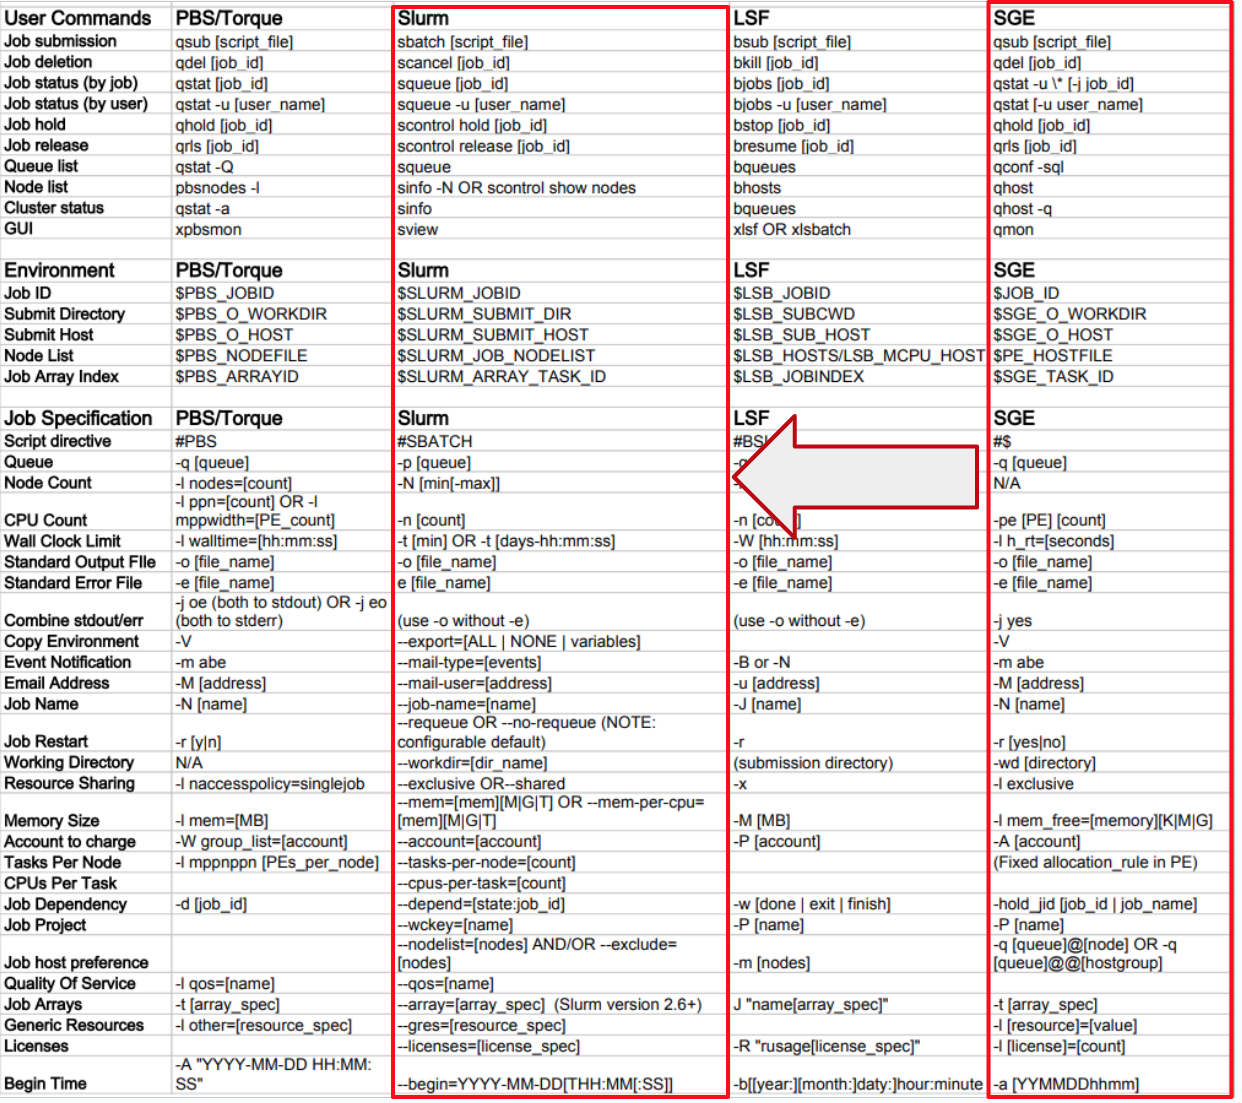
\includegraphics[width=\columnwidth]{images/rosetta-mapping}
    \caption{Rosetta Mappings of Scheduler Commands from SchedMD}
    \label{fig:rosetta-mappings}
\end{figure}

\item
\textbf{NOTE:} If you have used UGE commands in the past you probably still have these
lines there; \textbf{they should now be removed}, as they have no use in SLURM and
will start giving ``command not found'' errors on login when the software is removed:

csh/\tool{tcsh}: sample \file{.tcshrc} file:
\begin{verbatim}
    # Speed environment set up
    if ($HOSTNAME == speed-submit.encs.concordia.ca) then
    source /local/pkg/uge-8.6.3/root/default/common/settings.csh
    endif
\end{verbatim}

Bourne shell/\tool{bash}: sample \file{.bashrc} file:
\begin{verbatim}
    # Speed environment set up
    if [ $HOSTNAME = "speed-submit.encs.concordia.ca" ]; then
        . /local/pkg/uge-8.6.3/root/default/common/settings.sh
        printenv ORGANIZATION | grep -qw ENCS || . /encs/Share/bash/profile
    fi
\end{verbatim}

\textbf{IMPORTANT NOTE:} you will need to either log out and back in, or execute a new shell, 
for the environment changes in the updated \file{.tcshrc} or \file{.bashrc} file to be applied.
\end{itemize}

% A.3 Phases
% -------------------------------------------------------------
\subsection{Phases}
\label{sect:phases}

Brief summary of Speed evolution phases:

\subsubsection{Phase 5}
Phase 5 saw incorporation of the Salus, Magic, and Nebular
subclusters (see \xf{fig:speed-architecture-full}).

\subsubsection{Phase 4}
Phase 4 had 7 SuperMicro servers with 4x A100 80GB GPUs each added,
dubbed as ``SPEED2''. We also moved from Grid Engine to SLURM.

\subsubsection{Phase 3}
Phase 3 had 4 vidpro nodes added from Dr.~Amer totalling 6x P6 and 6x V100
GPUs added.

\subsubsection{Phase 2}
Phase 2 saw 6x NVIDIA Tesla P6 added and 8x more compute nodes.
The P6s replaced 4x of FirePro S7150.

\subsubsection{Phase 1}
Phase 1 of Speed was of the following configuration:
\begin{itemize}
    \item
    Sixteen, 32-core nodes, each with 512~GB of memory and approximately 1~TB of volatile-scratch disk space.
    \item
    Five AMD FirePro S7150 GPUs, with 8~GB of memory (compatible with the Direct X, OpenGL, OpenCL, and Vulkan APIs).
\end{itemize}

% Includes:
% A.1 Acknowledgments
% A.2 Migration from UGE to SLURM
% A.3 Phases

% B Frequently Asked Questions
% -------------------------------------------------------------
% -----------------------------------------------------------------------------
%						B Frequently Asked Questions
% -----------------------------------------------------------------------------
\section{Frequently Asked Questions}
\label{sect:faqs}

% B.1 Where do I learn about Linux?
% -------------------------------------------------------------
\subsection{Where do I learn about Linux?}
\label{sect:faqs-linux}

All Speed users are expected to have a basic understanding of Linux and its commonly used commands.
Here are some recommended resources:

\paragraph*{Software Carpentry}:
Software Carpentry provides free resources to learn software, including a workshop on the Unix shell.
Visit \href{https://software-carpentry.org/lessons/}{Software Carpentry Lessons} to learn more.

\paragraph*{Udemy}:
There are numerous Udemy courses, including free ones, that will help you learn Linux.
Active Concordia faculty, staff and students have access to Udemy courses.
A recommended starting point for beginners is the course ``Linux Mastery: Master the Linux Command Line in 11.5 Hours''.
Visit \href{https://www.concordia.ca/it/services/udemy.html}{Concordia's Udemy page} to learn how Concordians can access Udemy.

% B.2 How to bash shell on Speed?
% -------------------------------------------------------------
\subsection{How to use bash shell on Speed?}
\label{sect:faqs-bash}

This section provides comprehensive instructions on how to utilize the bash shell on the Speed cluster.

\subsubsection{How do I set bash as my login shell?}
To set your default login shell to bash on Speed, your login shell on all GCS servers must be changed to bash.
To make this change, create a ticket with the Service Desk (or email \texttt{help at concordia.ca}) to
request that bash become your default login shell for your ENCS user account on all GCS servers.

\subsubsection{How do I move into a bash shell on Speed?}
To move to the bash shell, type \textbf{bash} at the command prompt:
\begin{verbatim}
	[speed-submit] [/home/a/a_user] > bash
	bash-4.4$ echo $0
	bash
\end{verbatim}
\noindent\textbf{Note} how the command prompt changes from
``\verb![speed-submit] [/home/a/a_user] >!'' to ``\verb!bash-4.4$!'' after entering the bash shell.

\subsubsection{How do I use the bash shell in an interactive session on Speed?}
Below are examples of how to use \tool{bash} as a shell in your interactive job sessions
with both the \tool{salloc} and \tool{srun} commands.
\begin{itemize}
	\item \texttt{salloc -ppt --mem=100G -N 1 -n 10 /encs/bin/bash}
	\item \texttt{srun --mem=50G -n 5 --pty /encs/bin/bash}
\end{itemize}
\noindent\textbf{Note:} Make sure the interactive job requests memory, cores, etc.

\subsubsection{How do I run scripts written in bash on \tool{Speed}?}
To execute bash scripts on Speed:
\begin{enumerate}
	\item Ensure that the shebang of your bash job script is \verb+#!/encs/bin/bash+
	\item Use the \tool{sbatch} command to submit your job script to the scheduler.
\end{enumerate}
\noindent Check Speed GitHub for a \href{https://github.com/NAG-DevOps/speed-hpc/blob/master/src/bash.sh}{sample bash job script}.

% B.3 How to resolve “Disk quota exceeded” errors?
% -------------------------------------------------------------
\subsection{How to resolve ``Disk quota exceeded'' errors?}
\label{sect:quota-exceeded}

\subsubsection{Probable Cause}
The ``\texttt{Disk quota exceeded}'' error occurs when your application has
run out of disk space to write to. On \tool{Speed}, this error can be returned when:
\begin{enumerate}
	\item The NFS-provided home is full and cannot be written to.
	You can verify this using the \tool{quota} and \tool{bigfiles} commands.
	\item The ``\texttt{/tmp}'' directory on the speed node where your application is running is full and cannot be written to.
\end{enumerate}

\subsubsection{Possible Solutions}
\begin{enumerate}
	\item Use the \option{--chdir} job script option to set the job working directory.
	This is the directory where the job will write output files.

 	\item Although local disk space is recommended for IO-intensive operations, the 
 	`\texttt{/tmp}' directory on \tool{Speed} nodes is limited to 1TB, so it may be necessary 
	to store temporary data elsewhere. Review the documentation for each module
	used in your script to determine how to set working directories.
	The basic steps are:
	\begin{itemize}
	\item
	Determine how to set working directories for each module used in your job script.
	\item
	Create a working directory in \tool{speed-scratch} for output files:
	\begin{verbatim}
		mkdir -m 750 /speed-scratch/$USER/output
	\end{verbatim}
	\item
	Create a subdirectory for recovery files:
	\begin{verbatim}
		mkdir -m 750 /speed-scratch/$USER/recovery
	\end{verbatim}
	\item
	Update the job script to write output to the directories created in your \tool{speed-scratch} directory,
	e.g., \verb!/speed-scratch/$USER/output!.
	\end{itemize}
\end{enumerate}
\noindent In the above example, \verb!$USER! is an environment variable containing your ENCS username.

\subsubsection{Example of setting working directories for \tool{COMSOL}}
\begin{itemize}
	\item Create directories for recovery, temporary, and configuration files.
	\begin{verbatim}
		mkdir -m 750 -p /speed-scratch/$USER/comsol/{recovery,tmp,config}
	\end{verbatim}
	\item Add the following command switches to the COMSOL command to use the directories created above:
	\begin{verbatim}
		-recoverydir /speed-scratch/$USER/comsol/recovery
		-tmpdir /speed-scratch/$USER/comsol/tmp
		-configuration/speed-scratch/$USER/comsol/config
	\end{verbatim}
\end{itemize}
\noindent In the above example, \verb!$USER! is an environment variable containing your ENCS username.

\subsubsection{Example of setting working directories for \tool{Python Modules}}
By default when adding a Python module, the \texttt{/tmp} directory is set as the temporary repository for files downloads.
The size of the \texttt{/tmp} directory on \verb!speed-submit! is too small for PyTorch.
To add a Python module
\begin{itemize}
    \item Create your own tmp directory in your \verb!speed-scratch! directory:
	\begin{verbatim}
  		mkdir /speed-scratch/$USER/tmp
	\end{verbatim}
	\item Use the temporary directory you created
	\begin{verbatim}
  		setenv TMPDIR /speed-scratch/$USER/tmp
	\end{verbatim}
    \item Attempt the installation of PyTorch
\end{itemize}
\noindent In the above example, \verb!$USER! is an environment variable containing your ENCS username.

% B.4 How do I check my job's status?
% -------------------------------------------------------------
\subsection{How do I check my job's status?}
\label{sect:faq-job-status}

When a job with a job ID of 1234 is running or terminated, you can track its status using the following commands to check its status:
\begin{itemize}
	\item Use the ``sacct'' command to view the status of a job:
	\begin{verbatim}
		sacct -j 1234
	\end{verbatim}
	\item Use the ``squeue'' command to see if the job is sitting in the queue:
	\begin{verbatim}
		squeue -j 1234
	\end{verbatim}
	\item Use the ``sstat'' command to find long-term statistics on the job after it has terminated
	and the \tool{slurmctld} has purged it from its tracking state into the database:
	\begin{verbatim}
		sstat -j 1234
	\end{verbatim}
\end{itemize}

% B.5 Why is my job pending when nodes are empty?
% -------------------------------------------------------------
\subsection{Why is my job pending when nodes are empty?}

\subsubsection{Disabled nodes}
It is possible that one or more of the Speed nodes are disabled for maintenance.
To verify if Speed nodes are disabled, check if they are in a draining or drained state:

\small
\begin{verbatim}
[serguei@speed-submit src] % sinfo --long --Node
Thu Oct 19 21:25:12 2023
NODELIST   NODES PARTITION       STATE CPUS    S:C:T MEMORY TMP_DISK WEIGHT AVAIL_FE REASON
speed-01       1        pa        idle 32     2:16:1 257458        0      1    gpu16 none
speed-03       1        pa        idle 32     2:16:1 257458        0      1    gpu32 none
speed-05       1        pg        idle 32     2:16:1 515490        0      1    gpu16 none
speed-07       1       ps*       mixed 32     2:16:1 515490        0      1    cpu32 none
speed-08       1       ps*     drained 32     2:16:1 515490        0      1    cpu32 UGE
speed-09       1       ps*     drained 32     2:16:1 515490        0      1    cpu32 UGE
speed-10       1       ps*     drained 32     2:16:1 515490        0      1    cpu32 UGE
speed-11       1       ps*        idle 32     2:16:1 515490        0      1    cpu32 none
speed-12       1       ps*     drained 32     2:16:1 515490        0      1    cpu32 UGE
speed-15       1       ps*     drained 32     2:16:1 515490        0      1    cpu32 UGE
speed-16       1       ps*     drained 32     2:16:1 515490        0      1    cpu32 UGE
speed-17       1        pg     drained 32     2:16:1 515490        0      1    gpu16 UGE
speed-19       1       ps*        idle 32     2:16:1 515490        0      1    cpu32 none
speed-20       1       ps*     drained 32     2:16:1 515490        0      1    cpu32 UGE
speed-21       1       ps*     drained 32     2:16:1 515490        0      1    cpu32 UGE
speed-22       1       ps*     drained 32     2:16:1 515490        0      1    cpu32 UGE
speed-23       1       ps*        idle 32     2:16:1 515490        0      1    cpu32 none
speed-24       1       ps*        idle 32     2:16:1 515490        0      1    cpu32 none
speed-25       1        pg        idle 32     2:16:1 257458        0      1    gpu32 none
speed-25       1        pa        idle 32     2:16:1 257458        0      1    gpu32 none
speed-27       1        pg        idle 32     2:16:1 257458        0      1    gpu32 none
speed-27       1        pa        idle 32     2:16:1 257458        0      1    gpu32 none
speed-29       1       ps*        idle 32     2:16:1 515490        0      1    cpu32 none
speed-30       1       ps*     drained 32     2:16:1 515490        0      1    cpu32 UGE
speed-31       1       ps*     drained 32     2:16:1 515490        0      1    cpu32 UGE
speed-32       1       ps*     drained 32     2:16:1 515490        0      1    cpu32 UGE
speed-33       1       ps*        idle 32     2:16:1 515490        0      1    cpu32 none
speed-34       1       ps*        idle 32     2:16:1 515490        0      1    cpu32 none
speed-35       1       ps*     drained 32     2:16:1 515490        0      1    cpu32 UGE
speed-36       1       ps*     drained 32     2:16:1 515490        0      1    cpu32 UGE
speed-37       1        pt        idle 256    2:64:2 980275        0      1 gpu20,mi none
speed-38       1        pt        idle 256    2:64:2 980275        0      1 gpu20,mi none
speed-39       1        pt        idle 256    2:64:2 980275        0      1 gpu20,mi none
speed-40       1        pt        idle 256    2:64:2 980275        0      1 gpu20,mi none
speed-41       1        pt        idle 256    2:64:2 980275        0      1 gpu20,mi none
speed-42       1        pt        idle 256    2:64:2 980275        0      1 gpu20,mi none
speed-43       1        pt        idle 256    2:64:2 980275        0      1 gpu20,mi none
\end{verbatim}
\normalsize

\noindent Note which nodes are in the state of \textbf{drained}.
The reason for the drained state can be found in the \textbf{reason} column.
Your job will run once an occupied node becomes availble or the maintenance is completed,
and the disabled nodes have a state of \textbf{idle}.

\subsubsection{Error in job submit request.}
It is possible that your job is pending because it requested resources that are not available within Speed. 
To verify why job ID 1234 is not running, execute:
\begin{verbatim}
	sacct -j 1234
\end{verbatim}

\noindent A summary of the reasons can be obtained via the \tool{squeue} command.

% B.6 How to Handle /tmp Overflow on Speed Nodes?
% -------------------------------------------------------------
\subsection{How to Handle \tool{/tmp} Overflow on Speed Nodes?}
\label{sect:faq-tmp-on-speed}

Users may encounter a full \tool{/tmp} directory on Speed nodes when running LlamaIndex (or similar applications).
This happens when temporary files are written directly to \tool{/tmp} instead of a designated scratch space which causes job failures or system instability.

\subsubsection{Cause}
\begin{itemize}
	\item Hardcoded paths like "/tmp" in scripts can lead to issues.
	\item LlamaIndex (and other ML-related tools) may default to storing temporary and cache files in \tool{/tmp}.
\end{itemize}

\subsubsection{Solution}
\begin{itemize}

	\item Use \tool{TMPDIR} instead of \tool{/tmp} to set a temporary directory for your job 
		as \tool{TMPDIR} maps to \tool{/nobackup} or \tool{/nobackup2} which have more storage.
		\begin{verbatim}
			setenv TMP $TMPDIR
			setenv TEMP $TMPDIR
		\end{verbatim}

	\item Set cache and temporary directories in your script.
		\begin{itemize}
			\item Example fix for LlamaIndex:
			\begin{verbatim}
				mkdir -p $TMPDIR/$USER
				setenv LLAMA_INDEX_CACHE_DIR $TMPDIR/$USER
			\end{verbatim}
		\end{itemize}

	\item Ensure the Python script uses the correct temporary directory
		\begin{itemize}
			\item Example fix for Chromadb in LlamaIndex:
			\begin{verbatim}
				db_path = os.path.join(os.getenv("TMPDIR"), "db")
				db = chromadb.PersistentClient(path=db_path)
			\end{verbatim}
		\end{itemize}

\end{itemize}
% TO DELETE
%% ------------------------------------------------------------------------------
%						B Frequently Asked Questions 
% ------------------------------------------------------------------------------
\section{Frequently Asked Questions}
\label{sect:faqs}

% B.1 Where do I learn about Linux?
% -------------------------------------------------------------
\subsection{Where do I learn about Linux?}
\label{sect:faqs-linux}

All Speed users are expected to have a basic understanding of Linux and its commonly used commands.
Here are some recommended resources:

\paragraph*{Software Carpentry}
Software Carpentry provides free resources to learn software, including a workshop on the Unix shell.
Visit \href{https://software-carpentry.org/lessons/}{Software Carpentry Lessons} to learn more.

\paragraph*{Udemy}
There are numerous Udemy courses, including free ones, that will help you learn Linux. 
Active Concordia faculty, staff and students have access to Udemy courses. 
A recommended starting point for beginners is the course ``Linux Mastery: Master the Linux Command Line in 11.5 Hours''.
Visit \href{https://www.concordia.ca/it/services/udemy.html}{Concordia's Udemy page} to learn how Concordians can access Udemy.

% B.2 How to bash shell on Speed?
% -------------------------------------------------------------
\subsection{How to use bash shell on \tool{Speed}?}
\label{sect:faqs-bash}

This section provides comprehensive instructions on how to utilize the bash shell on the Speed cluster.

% B.2.1 How do I set bash as my login shell?
\subsubsection{How do I set bash as my login shell?}
To set your default login shell to bash on Speed, your login shell on all GCS servers must be changed to bash.
To make this change, create a ticket with the Service Desk (or email \texttt{help at concordia.ca}) to
request that bash become your default login shell for your ENCS user account on all GCS servers.

% B.2.2 How do I move into a bash shell on Speed?
\subsubsection{How do I move into a bash shell on \tool{Speed}?}
To move to the bash shell, type \textbf{bash} at the command prompt:
\begin{verbatim}
	[speed-submit] [/home/a/a_user] > bash
	bash-4.4$ echo $0
	bash
\end{verbatim}	

\noindent \textbf{Note} how the command prompt changes from 
``\verb![speed-submit] [/home/a/a_user] >!'' to ``\verb!bash-4.4$!'' after entering the bash shell.

% B.2.3 How do I use the bash shell in an interactive session on Speed?
\subsubsection{How do I use the bash shell in an interactive session on \tool{Speed}?}
Below are examples of how to use \tool{bash} as a shell in your interactive job sessions 
with both the \tool{salloc} and \tool{srun} commands.

\begin{itemize}
	\item \texttt{salloc -ppt --mem=100G -N 1 -n 10 /encs/bin/bash}
	\item \texttt{srun  --mem=50G -n 5 --pty /encs/bin/bash}
\end{itemize}

\noindent\textbf{Note:} Make sure the interactive job requests memory, cores, etc.

% B.2.4 How do I run scripts written in bash on Speed?
\subsubsection{How do I run scripts written in bash on \tool{Speed}?}

To execute bash scripts on Speed:
\begin{enumerate}
	\item Ensure that the shebang of your bash job script is \verb+#!/encs/bin/bash+
	\item Use the \tool{sbatch} command to submit your job script to the scheduler.
\end{enumerate}

\noindent Check Speed GitHub for a 
\href{https://github.com/NAG-DevOps/speed-hpc/blob/master/src/bash.sh}{sample bash job script}.

% B.3 How to resolve “Disk quota exceeded” errors?
% -------------------------------------------------------------
\subsection{How to resolve ``Disk quota exceeded'' errors?}

% B.3.1 Probable Cause
\subsubsection{Probable Cause}

The ``\texttt{Disk quota exceeded}'' error occurs when your application has 
run out of disk space to write to. On \tool{Speed}, this error can be returned when:
\begin{enumerate}
	\item The NFS-provided home is full and cannot be written to.
	You can verify this using the \tool{quota} and \tool{bigfiles} commands.
	\item The ``\texttt{/tmp}'' directory on the speed node where your application is running is full and cannot be written to.
\end{enumerate}

% B.3.2 Possible Solutions
\subsubsection{Possible Solutions}

\begin{enumerate}
	\item Use the \option{--chdir} job script option to set the job working directory.
	This is the directory where the job will write output files.

 	\item Although local disk space is recommended for IO-intensive operations, the 
 	`\texttt{/tmp}' directory on \tool{Speed} nodes is limited to 1TB, so it may be necessary 
	to store temporary data elsewhere. Review the documentation for each module
	used in your script to determine how to set working directories.
	The basic steps are:
	\begin{itemize}
		\item
		Determine how to set working directories for each module used in your job script.
		\item
		Create a working directory in \tool{speed-scratch} for output files:
		\begin{verbatim}
			mkdir -m 750 /speed-scratch/$USER/output
		\end{verbatim}
		\item
		Create a subdirectory for recovery files:
		\begin{verbatim}
			mkdir -m 750 /speed-scratch/$USER/recovery
		\end{verbatim}
		\item
		Update the job script to write output to the directories created in your 
		\tool{speed-scratch} directory, e.g., \verb!/speed-scratch/$USER/output!.
	\end{itemize}
\end{enumerate}
\noindent In the above example, \verb!$USER! is an environment variable containing your ENCS username.

% B.3.3 Example of setting working directories for COMSOL
\subsubsection{Example of setting working directories for \tool{COMSOL}}

\begin{itemize}
	\item Create directories for recovery, temporary, and configuration files. 
	\begin{verbatim}
		mkdir -m 750 -p /speed-scratch/$USER/comsol/{recovery,tmp,config}
	\end{verbatim}
	\item Add the following command switches to the COMSOL command to use the 
	directories created above:
	\begin{verbatim} 
		-recoverydir /speed-scratch/$USER/comsol/recovery 
		-tmpdir /speed-scratch/$USER/comsol/tmp
		-configuration/speed-scratch/$USER/comsol/config
	\end{verbatim}
\end{itemize} 
\noindent In the above example, \verb!$USER! is an environment variable containing your ENCS username.

% B.3.4 Example of setting working directories for Python Modules
\subsubsection{Example of setting working directories for \tool{Python Modules}}

By default when adding a Python module, the \texttt{/tmp} directory is set as the temporary repository for files downloads.
The size of the \texttt{/tmp} directory on \verb!speed-submit! is too small for PyTorch.
To add a Python module
\begin{itemize}
    \item Create your own tmp directory in your \verb!speed-scratch! directory:
	\begin{verbatim} 
  		mkdir /speed-scratch/$USER/tmp
	\end{verbatim}
	\item Use the temporary directory you created
	\begin{verbatim} 
  		setenv TMPDIR /speed-scratch/$USER/tmp
	\end{verbatim}
    \item Attempt the installation of PyTorch
\end{itemize}
\noindent In the above example, \verb!$USER! is an environment variable containing your ENCS username.

% B.4 How do I check my job's status?
% -------------------------------------------------------------
\subsection{How do I check my job's status?}

%When a job with a job id of 1234 is running, the status of that job can be tracked using \verb!`qstat -j 1234`!.
%Likewise, if the job is pending, the \verb!`qstat -j 1234`! command will report as to why the job is not scheduled or running.
%Once the job has finished, or has been killed, the \textbf{qacct} command must be used to query the job's status, e.g., \verb!`qaact -j [jobid]`!. 
When a job with a job ID of 1234 is running or terminated, 
you can track its status using the following commands:
\begin{itemize}
	\item Use the ``sacct'' command to view the status of a job:
	\begin{verbatim} 
		sacct -j 1234
	\end{verbatim}
	\item Use the ``squeue'' command to see if the job is sitting in the queue:
	\begin{verbatim} 
		squeue -j 1234
	\end{verbatim}
	\item Use the ``sstat'' command to find long-term statistics on the job after it has terminated 
	and the \tool{slurmctld} has purged it from its tracking state into the database:
	\begin{verbatim} 
		sstat -j 1234
	\end{verbatim}
\end{itemize}

% B.5 Why is my job pending when nodes are empty?
% -------------------------------------------------------------
\subsection{Why is my job pending when nodes are empty?}

% B.5.1 Disabled nodes
\subsubsection{Disabled nodes}
It is possible that one or more of the Speed nodes are disabled for maintenance.
To verify if Speed nodes are disabled, check if they are in a draining or drained state:

%\begin{verbatim}
%qstat -f -qs d
%queuename                      qtype resv/used/tot. load_avg arch          states
%---------------------------------------------------------------------------------
%g.q@speed-05.encs.concordia.ca BIP   0/0/32         0.27     lx-amd64      d
%---------------------------------------------------------------------------------
%s.q@speed-07.encs.concordia.ca BIP   0/0/32         0.01     lx-amd64      d
%---------------------------------------------------------------------------------
%s.q@speed-10.encs.concordia.ca BIP   0/0/32         0.01     lx-amd64      d
%---------------------------------------------------------------------------------
%s.q@speed-16.encs.concordia.ca BIP   0/0/32         0.02     lx-amd64      d
%---------------------------------------------------------------------------------
%s.q@speed-19.encs.concordia.ca BIP   0/0/32         0.03     lx-amd64      d
%---------------------------------------------------------------------------------
%s.q@speed-24.encs.concordia.ca BIP   0/0/32         0.01     lx-amd64      d
%---------------------------------------------------------------------------------
%s.q@speed-36.encs.concordia.ca BIP   0/0/32         0.03     lx-amd64      d
%\end{verbatim}

\small
\begin{verbatim}
[serguei@speed-submit src] % sinfo --long --Node
Thu Oct 19 21:25:12 2023
NODELIST   NODES PARTITION       STATE CPUS    S:C:T MEMORY TMP_DISK WEIGHT AVAIL_FE REASON
speed-01       1        pa        idle 32     2:16:1 257458        0      1    gpu16 none
speed-03       1        pa        idle 32     2:16:1 257458        0      1    gpu32 none
speed-05       1        pg        idle 32     2:16:1 515490        0      1    gpu16 none
speed-07       1       ps*       mixed 32     2:16:1 515490        0      1    cpu32 none
speed-08       1       ps*     drained 32     2:16:1 515490        0      1    cpu32 UGE
speed-09       1       ps*     drained 32     2:16:1 515490        0      1    cpu32 UGE
speed-10       1       ps*     drained 32     2:16:1 515490        0      1    cpu32 UGE
speed-11       1       ps*        idle 32     2:16:1 515490        0      1    cpu32 none
speed-12       1       ps*     drained 32     2:16:1 515490        0      1    cpu32 UGE
speed-15       1       ps*     drained 32     2:16:1 515490        0      1    cpu32 UGE
speed-16       1       ps*     drained 32     2:16:1 515490        0      1    cpu32 UGE
speed-17       1        pg     drained 32     2:16:1 515490        0      1    gpu16 UGE
speed-19       1       ps*        idle 32     2:16:1 515490        0      1    cpu32 none
speed-20       1       ps*     drained 32     2:16:1 515490        0      1    cpu32 UGE
speed-21       1       ps*     drained 32     2:16:1 515490        0      1    cpu32 UGE
speed-22       1       ps*     drained 32     2:16:1 515490        0      1    cpu32 UGE
speed-23       1       ps*        idle 32     2:16:1 515490        0      1    cpu32 none
speed-24       1       ps*        idle 32     2:16:1 515490        0      1    cpu32 none
speed-25       1        pg        idle 32     2:16:1 257458        0      1    gpu32 none
speed-25       1        pa        idle 32     2:16:1 257458        0      1    gpu32 none
speed-27       1        pg        idle 32     2:16:1 257458        0      1    gpu32 none
speed-27       1        pa        idle 32     2:16:1 257458        0      1    gpu32 none
speed-29       1       ps*        idle 32     2:16:1 515490        0      1    cpu32 none
speed-30       1       ps*     drained 32     2:16:1 515490        0      1    cpu32 UGE
speed-31       1       ps*     drained 32     2:16:1 515490        0      1    cpu32 UGE
speed-32       1       ps*     drained 32     2:16:1 515490        0      1    cpu32 UGE
speed-33       1       ps*        idle 32     2:16:1 515490        0      1    cpu32 none
speed-34       1       ps*        idle 32     2:16:1 515490        0      1    cpu32 none
speed-35       1       ps*     drained 32     2:16:1 515490        0      1    cpu32 UGE
speed-36       1       ps*     drained 32     2:16:1 515490        0      1    cpu32 UGE
speed-37       1        pt        idle 256    2:64:2 980275        0      1 gpu20,mi none
speed-38       1        pt        idle 256    2:64:2 980275        0      1 gpu20,mi none
speed-39       1        pt        idle 256    2:64:2 980275        0      1 gpu20,mi none
speed-40       1        pt        idle 256    2:64:2 980275        0      1 gpu20,mi none
speed-41       1        pt        idle 256    2:64:2 980275        0      1 gpu20,mi none
speed-42       1        pt        idle 256    2:64:2 980275        0      1 gpu20,mi none
speed-43       1        pt        idle 256    2:64:2 980275        0      1 gpu20,mi none
\end{verbatim}
\normalsize

\noindent Note which nodes are in the state of \textbf{drained}.
The reason for the drained state can be found in the \textbf{reason} column.\\

\noindent Your job will run once an occupied node becomes availble or the maintenance is completed, 
and the disabled nodes have a state of \textbf{idle}.

% B.5.2 Error in job submit request.
\subsubsection{Error in job submit request.}

It is possible that your job is pending because it requested resources that are not available within Speed. 
To verify why job ID 1234 is not running, execute:
\begin{verbatim} 
	sacct -j 1234
\end{verbatim}

\noindent A summary of the reasons can be obtained via the \tool{squeue} command.
%and review the messages in the \textbf{scheduling info:} section.


% Includes:
% B.1 Where do I learn about Linux?
% B.2 How to bash shell on Speed?
% B.3 How to resolve “Disk quota exceeded” errors?
% B.4 How do I check my job's status?
% B.5 Why is my job pending when nodes are empty?

% C Sister Facilities
% -------------------------------------------------------------
% -----------------------------------------------------------------------------
%						C Sister Facilities
% -----------------------------------------------------------------------------

Below is a list of resources and facilities similar to Speed at various capacities.
Depending on your research group and needs, they might be available to you. They
are not managed by HPC/NAG of AITS, so contact their respective representatives.

\begin{itemize}
    \item
    \texttt{computation.encs} is a CPU-only 3-machine cluster running longer jobs without
    a scheduler at the moment. Shares the same EL7 software tree as Speed's EL7 nodes
    as well as lab desktops. See \url{https://www.concordia.ca/ginacody/aits/public-servers.html}.

    \item
    \texttt{apini.encs} cluster for teaching and MPI programming (see the corresponding
    course in CSSE), managed by CSSE.

    \item
    Computer Science and Software Engineering (CSSE) Virya GPU Cluster. For CSSE
    members only. The cluster has 4 nodes with total of 32 NVIDIA GPUs (a mix of
    V100s and A100s). To request access send email to \texttt{virya.help AT concordia.ca}.
    This includes an Atlas Analytics partition of Dr.~Mahdi Husseini.

    \item
    Dr.~Eugene Belilovsky hightower Exxact, and megatower graphcore clusters.

    \item
    Dr.~Maria Amer's VidPro group's nodes in Speed (-01, -03, -25, -27) with additional V100 and P6 GPUs.

    \item
    There are various Lambda Labs other GPU servers and like computers
    acquired by individual researchers; if you are member of their
    research group, contact them directly. These resources are not
    managed by us.

    \begin{itemize}
        \item Dr.~Amin Hammad's \texttt{construction.encs} Lambda Labs station
        \item Dr.~Hassan Rivaz's \texttt{impactlab.encs} Lambda Labs station
        \item Dr.~Nizar Bouguila's \texttt{xailab.encs} Lambda Labs station
        \item Dr.~Roch Glitho's \texttt{femto.encs} server
        \item Dr.~Maria Amer's \texttt{venom.encs} Lambda Labs station
        \item Dr.~Leon Wang's \texttt{guerrera.encs} DGX station
    \end{itemize}

    \item
    Dr.~Ivan Contreras' 4 Operations Research group servers (managed by AITS).

    \item
    If you are a member of School of Health (formerly PERFORM Center),
    you may have access to their local
    \href{https://perform-wiki.concordia.ca/mediawiki/index.php/HPC_Cluster}{PERFORM's High Performance Computing (HPC) Cluster}.
    Contact Thomas Beaudry for details and how to obtain access.

    \item
    All Concordia students have access to the Library's small
    \href{https://library.concordia.ca/technology/sandbox/}{Technology Sandbox}
    testing cluster that also runs Slurm. Email \texttt{sean.cooney AT concordia.ca} for details.

    \item
    Digital Research Alliance Canada (Compute Canada / Calcul Quebec),\\
    \url{https://alliancecan.ca/}. Follow
    \href{https://alliancecan.ca/en/services/advanced-research-computing/account-management/apply-account}{this link}
    on the information how to obtain access (students need to be sponsored
    by their supervising faculty members, who should create accounts first).
    Their SLURM examples are here: \url{https://docs.alliancecan.ca/wiki/Running_jobs}

\end{itemize}

% D Software List
% -------------------------------------------------------------
% -----------------------------------------------------------------------------
% ./generate-software-list.sh
\section{Software Installed On Speed}
\label{sect:software-details}

This is a generated section by a script; last updated on \textit{Tue Jul 23 10:22:01 PM EDT 2024}.
We have two major software trees: Scientific Linux 7 (EL7), which is
outgoing, and AlmaLinux 9 (EL9). After major synchronization of software
packages is complete, we will stop maintaining the EL7 tree and
will migrade the remaining nodes to EL9.

\noindent
\textbf{NOTE:} this list does not include packages installed directly on the OS (yet).

% -----------------------------------------------------------------------------
\subsection{EL7}
\label{sect:software-el7}

Not all packages are intended for HPC, but the common tree is available
on Speed as well as teaching labs' desktops.

\begin{multicols}{3}
\begin{itemize}
\item \verb|a2ps-4.13b|
\item \verb|a2ps-4.14|
\item \verb|abaqus-2019|
\item \verb|abaqus-2020|
\item \verb|abaqus-2021|
\item \verb|abaqus-2023|
\item \verb|acl-10.0.express|
\item \verb|acl-10.1.express|
\item \verb|acroread-9.5.5|
\item \verb|ADS-2016.01|
\item \verb|ADS-2017.01|
\item \verb|ADS-2019|
\item \verb|ADS-2020u1|
\item \verb|adt_bundle-20140702|
\item \verb|alpine-2.00|
\item \verb|alpine-2.25|
\item \verb|anaconda-1.7.0|
\item \verb|anaconda2-2019.07|
\item \verb|anaconda2-5.1.0|
\item \verb|anaconda3-2019.07|
\item \verb|anaconda3-2019.10|
\item \verb|anaconda3-2021.05|
\item \verb|anaconda3-2023.03|
\item \verb|anaconda3-5.1.0|
\item \verb|android_sdk-24.4.1|
\item \verb|android_studio-162.4069837|
\item \verb|android_studio-173.4720617|
\item \verb|ansoft_designer-6.1.2|
\item \verb|ansoft_designer-8.0|
\item \verb|ansys-16.2|
\item \verb|ansys-17.2|
\item \verb|ansys-18.2|
\item \verb|ansys-19.2|
\item \verb|ansys-2019R3|
\item \verb|ansys-2020R2|
\item \verb|ansys-2021R1|
\item \verb|ansys-2021R2|
\item \verb|ansys-2022R1|
\item \verb|ansys-2022R2|
\item \verb|ansys-2023R1|
\item \verb|ansys-2023R2|
\item \verb|AnsysEM-16.2|
\item \verb|ant-1.10.11|
\item \verb|ant-1.10.2|
\item \verb|ant-1.6.2|
\item \verb|ant-1.9.7|
\item \verb|ANTs-2.3.5|
\item \verb|ApacheDirectoryStudio-1.5.3|
\item \verb|arduino-1.6.8|
\item \verb|ArgoUML-0.34|
\item \verb|arpack-3.0.2|
\item \verb|ARWpost-3.1|
\item \verb|aspectj-1.7.0.M1|
\item \verb|aspectj-1.8.2|
\item \verb|aspectj-1.8.6|
\item \verb|aspell-0.60.6|
\item \verb|aspell-0.60.8|
\item \verb|atanua-1.2.130617|
\item \verb|autoconf-2.68|
\item \verb|autoconf-2.71|
\item \verb|AutoDock-4.2.6|
\item \verb|autogen-5.18.4|
\item \verb|automake-1.13.1|
\item \verb|automake-1.16.1|
\item \verb|autoson-1.4.3|
\item \verb|babl-0.1.12|
\item \verb|bash-4.4|
\item \verb|basilisk-19_3_23|
\item \verb|bazel-0.2.0|
\item \verb|bazel-0.21.0|
\item \verb|bazel-0.24.1|
\item \verb|bazel-0.26.1|
\item \verb|bazel-2.0.0|
\item \verb|bazel-3.7.2|
\item \verb|bazel-4.2.1|
\item \verb|bison-2.7.1|
\item \verb|bison-3.7.2|
\item \verb|blas-3.10.0|
\item \verb|blender-2.66a|
\item \verb|blender-2.78|
\item \verb|blender-2.78c|
\item \verb|bogofilter-1.2.4|
\item \verb|booksim-2.0|
\item \verb|boost-1.51.0|
\item \verb|boost-1.62.0|
\item \verb|boost-1.68.0|
\item \verb|boost-1.69.0|
\item \verb|boost-1.70.0|
\item \verb|boost-1.73.0|
\item \verb|bouncer-2.2|
\item \verb|buddy-2.4|
\item \verb|bzr-2.6.0|
\item \verb|camlp5-6.02.3|
\item \verb|camlp5-6.14|
\item \verb|CGAL-4.3|
\item \verb|cgiwrap-4.1|
\item \verb|Check-0.15.2|
\item \verb|chrome-101.0.4951.54|
\item \verb|chromium-31.0.1650.63|
\item \verb|cilkplus-4.8|
\item \verb|clips-6.23|
\item \verb|clips-6.30|
\item \verb|clojure-1.8.0|
\item \verb|cmake-2.8.12|
\item \verb|cmake-3.18.4|
\item \verb|cmake-3.26.4|
\item \verb|cmake-3.8.2|
\item \verb|CMC_utils-1.0|
\item \verb|codeblocks-13.12|
\item \verb|codelite-9.1|
\item \verb|comsol-3.5a|
\item \verb|comsol-4.0|
\item \verb|comsol-4.1|
\item \verb|comsol-5.6|
\item \verb|comsol-6.0|
\item \verb|comsol-6.1|
\item \verb|concorde-20031219|
\item \verb|coware-2010.1|
\item \verb|cplex-12.10.0|
\item \verb|cplex-12.6.1|
\item \verb|cplex-12.6.2|
\item \verb|cplex-12.6.3|
\item \verb|cplex-12.7.0|
\item \verb|cplex-12.7.1|
\item \verb|cplex-12.8.0|
\item \verb|cplex-12.9.0|
\item \verb|cplex-20.1.0|
\item \verb|cplex-22.1.0|
\item \verb|cplex-22.1.1|
\item \verb|cppunit-1.13.2|
\item \verb|CST-2014|
\item \verb|CST-2019|
\item \verb|CST-2020|
\item \verb|cuda-10.0|
\item \verb|cuda-10.2|
\item \verb|cuda-11.5|
\item \verb|cuda-11.8|
\item \verb|cuda-9.2|
\item \verb|cups-1.3.7|
\item \verb|cups-2.3.3|
\item \verb|curl-7.15.0|
\item \verb|curl-7.38.0|
\item \verb|curl-7.73.0|
\item \verb|curl-7.84.0|
\item \verb|curl-7.86.0|
\item \verb|curl-7.87.0|
\item \verb|curl-8.1.2|
\item \verb|cvs-1.11.23|
\item \verb|cvx-2.1|
\item \verb|DbVisualizer-24.1.5|
\item \verb|DbVisualizer-9.1.9|
\item \verb|ddd-3.3.12|
\item \verb|dejagnu-1.5.3|
\item \verb|dejagnu-1.6.2|
\item \verb|digilent-2.19.2|
\item \verb|digilent-2.8.2|
\item \verb|dmtcp-1.2.8|
\item \verb|dos2unix-7.3|
\item \verb|doxygen-1.8.4|
\item \verb|drush-6.5.0|
\item \verb|ece-eclipse-jee.juno|
\item \verb|ece-eclipse-jee.luna|
\item \verb|ecj-25|
\item \verb|ECLiPSe-6.0_192|
\item \verb|eclipse-jee.201812|
\item \verb|eclipse-jee.202003|
\item \verb|eclipse-jee.202109|
\item \verb|eclipse-jee.202209|
\item \verb|eclipse-jee.indigo|
\item \verb|eclipse-jee.juno|
\item \verb|eclipse-jee.luna|
\item \verb|eclipse-jee.mars|
\item \verb|eclipse-jee.neon|
\item \verb|eclipse-jee.oxygen|
\item \verb|eigen-3.3.7|
\item \verb|electromagnetics_suite-2022R2|
\item \verb|electromagnetics_suite-2023R1|
\item \verb|emacs-24.4|
\item \verb|emacs-25.2|
\item \verb|enscript-1.6.5.2|
\item \verb|exmh-2.7.0|
\item \verb|expat-2.1.0|
\item \verb|expect-5.45|
\item \verb|expect-5.45.4|
\item \verb|fanout-0.6.1|
\item \verb|feko-2017.2.2|
\item \verb|feko-2018.2|
\item \verb|feko-6.1|
\item \verb|feko-7.0.1|
\item \verb|ffmpeg-0.10.2|
\item \verb|ffmpeg-3.3.2|
\item \verb|ffmpeg-4.1.3|
\item \verb|fftw-3.2.2|
\item \verb|fftw-3.3.10|
\item \verb|fftw-3.3.8|
\item \verb|firefox-102.11.0|
\item \verb|firefox-102.12.0|
\item \verb|firefox-102.13.0|
\item \verb|firefox-102.14.0|
\item \verb|firefox-102.15.0|
\item \verb|firefox-102.15.1|
\item \verb|firefox-115.10.0|
\item \verb|firefox-115.2.1|
\item \verb|firefox-115.3.0|
\item \verb|firefox-17.0.11|
\item \verb|firefox-2.0.0.20|
\item \verb|firefox-24.8.1|
\item \verb|firefox-31.7.0|
\item \verb|firefox-38.8.0|
\item \verb|firefox-45.9.0|
\item \verb|firefox-52.9.0|
\item \verb|firefox-60.9.0|
\item \verb|firefox-68.12.0|
\item \verb|firefox-78.15.0|
\item \verb|firefox-91.11.0|
\item \verb|firefox_french-102.11.0|
\item \verb|firefox_french-102.12.0|
\item \verb|firefox_french-102.13.0|
\item \verb|firefox_french-102.14.0|
\item \verb|firefox_french-102.15.0|
\item \verb|firefox_french-102.15.1|
\item \verb|firefox_french-115.10.0|
\item \verb|firefox_french-115.2.1|
\item \verb|firefox_french-115.3.0|
\item \verb|firefox_french-24.8.1|
\item \verb|firefox_french-31.7.0|
\item \verb|firefox_french-38.8.0|
\item \verb|firefox_french-45.9.0|
\item \verb|firefox_french-52.9.0|
\item \verb|firefox_french-60.9.0|
\item \verb|firefox_french-68.12.0|
\item \verb|firefox_french-78.15.0|
\item \verb|firefox_french-91.11.0|
\item \verb|flex-2.5.37|
\item \verb|flex-2.6.4|
\item \verb|fltk-1.3.2|
\item \verb|fltk-1.3.8|
\item \verb|fox-1.6.49|
\item \verb|FreeImage-3.18.0|
\item \verb|freerdp-1.0.2|
\item \verb|freerdp-1.2.0|
\item \verb|freetype-2.4.12|
\item \verb|FSL-6.0.5|
\item \verb|fsl-6.0.6.2|
\item \verb|fsr-1.9|
\item \verb|fxscintilla-2.28.0|
\item \verb|gambit-c-4.7.5|
\item \verb|gate-7.1|
\item \verb|gc-7.2f|
\item \verb|gcc-12.2.0|
\item \verb|gcc-13.1.0|
\item \verb|gcc-3.3.2|
\item \verb|gcc-4.1.2|
\item \verb|gcc-4.4.3|
\item \verb|gcc-4.7.2|
\item \verb|gcc-4.9.2|
\item \verb|gcc-5.1.0|
\item \verb|gcc-5.2.0|
\item \verb|gcc-5.4.0|
\item \verb|gcc-6.1.0|
\item \verb|gcc-7.3.0|
\item \verb|gcc-8.4.0|
\item \verb|gcc-9.2.0|
\item \verb|gcc-9.3.0|
\item \verb|gcc-arm-11.2.2022.02|
\item \verb|gdb-12.1|
\item \verb|gdb-7.7|
\item \verb|geomview-1.9.4|
\item \verb|gerris-131206|
\item \verb|getmail-4.54.0|
\item \verb|gettext-0.18.1.1|
\item \verb|gfsview-121130|
\item \verb|ghc-7.6.3|
\item \verb|ghostscript-10.0.0|
\item \verb|ghostscript-8.50|
\item \verb|ghostscript-9.25|
\item \verb|ghostscript-9.26|
\item \verb|ghostscript-9.50|
\item \verb|ghostscript-9.52|
\item \verb|gifsicle-1.92|
\item \verb|gimp-2.8.14|
\item \verb|gimp-2.8.18|
\item \verb|git-1.8.5.3|
\item \verb|git-2.15.0|
\item \verb|git-2.22.0|
\item \verb|git-2.23.0|
\item \verb|git-2.23.3|
\item \verb|git-2.29.2|
\item \verb|git-2.35.1|
\item \verb|git-2.5.0|
\item \verb|gl2ps-1.3.8|
\item \verb|glade3-3.8.3|
\item \verb|glew-1.10.0|
\item \verb|glew-2.1.0|
\item \verb|glfw-3.0.4|
\item \verb|glfw-3.3|
\item \verb|glfw-3.3.4|
\item \verb|glm-0.9.5.4|
\item \verb|glm-0.9.9.8|
\item \verb|glpk-4.55|
\item \verb|gmp-4.3.2|
\item \verb|gnome_env-20110618|
\item \verb|gnome_env-20130510|
\item \verb|gnupg-2.3.4|
\item \verb|gnuplot-4.6.3|
\item \verb|gnuplot-5.0.1|
\item \verb|gnuplot-5.0.3|
\item \verb|go-1.10.2|
\item \verb|go-1.12|
\item \verb|go-1.15.6|
\item \verb|go-1.19.3|
\item \verb|go-1.3|
\item \verb|go-1.9|
\item \verb|GoldenGate-2020u1|
\item \verb|gperf-3.0.4|
\item \verb|grace-5.1.25|
\item \verb|GraphiteTwo-a5|
\item \verb|GraphiteTwo-Concordia_v1|
\item \verb|graphviz-2.30.0|
\item \verb|graphviz-2.40.1|
\item \verb|gromacs-5.0.7|
\item \verb|gsl-2.6|
\item \verb|gtkwave-3.3.15|
\item \verb|gts-121130|
\item \verb|guile-2.0.11|
\item \verb|gurobi-10.0.0|
\item \verb|gurobi-10.0.1|
\item \verb|gurobi-7.0.1|
\item \verb|gurobi-7.5.0|
\item \verb|gurobi-8.0.0|
\item \verb|gurobi-8.1.0|
\item \verb|gurobi-9.0.0|
\item \verb|gurobi-9.0.2|
\item \verb|gurobi-9.1.0|
\item \verb|gurobi-9.5.0|
\item \verb|gurobi-9.5.2|
\item \verb|gv-3.7.4|
\item \verb|hadoop-1.0.4|
\item \verb|hadoop-1.1.2|
\item \verb|hadoop-2.4.1|
\item \verb|hadoop-2.7.1|
\item \verb|hadoop-2.7.3|
\item \verb|hadoop-2.9.0|
\item \verb|haskell_platform-2013.2.0.0|
\item \verb|hdf5-1.10.5|
\item \verb|hdf5-1.8.11|
\item \verb|hexpert-2.4.1|
\item \verb|hmmer-3.3.2|
\item \verb|html2ps-1.0b5|
\item \verb|httpd-2.2.22|
\item \verb|httpd-2.2.32|
\item \verb|httpd-2.4.27|
\item \verb|httpd-2.4.38|
\item \verb|httpd-2.4.39|
\item \verb|httpd-2.4.52|
\item \verb|httpd-2.4.53|
\item \verb|httpd-2.4.54|
\item \verb|httpd-2.4.55|
\item \verb|httpd-2.4.57|
\item \verb|httpd-current|
\item \verb|http-parser-2.9.4|
\item \verb|hunspell-1.7.2|
\item \verb|hwloc-1.11.2|
\item \verb|hwloc-2.8.0|
\item \verb|hxplay-11.0.2|
\item \verb|hyperworks-12.0|
\item \verb|iBioSim-3.0.0.beta|
\item \verb|ImageMagick-6.3.6|
\item \verb|ImageMagick-6.9.4.1|
\item \verb|ImageMagick-7.0.8.42|
\item \verb|imap-2007e|
\item \verb|instantclient-19.3.0.0.0|
\item \verb|IntelliJ-2019.2.3|
\item \verb|intltool-0.50.2|
\item \verb|invtools-2.0|
\item \verb|invtools-2.0.2|
\item \verb|invtools-2.1.0|
\item \verb|invtools-2.2.0|
\item \verb|invtools-2.3.0|
\item \verb|invtools-2.4.0|
\item \verb|invtools-2.5.0|
\item \verb|invtools-2.5.1|
\item \verb|invtools-2.6.0|
\item \verb|invtools-2.7.0|
\item \verb|invtools-2.8.0|
\item \verb|invtools-3.0.0|
\item \verb|invtools-3.1.0|
\item \verb|ipe-7.1.3|
\item \verb|iq-8.4.1|
\item \verb|j2sdk_32b-1.5.0_22|
\item \verb|j2sdk_64b-1.5.0_22|
\item \verb|jansson-2.14|
\item \verb|jdk-11|
\item \verb|jdk-11.0.1|
\item \verb|jdk-11.0.2|
\item \verb|jdk-17|
\item \verb|jdk-17.0.2|
\item \verb|jdk-19|
\item \verb|jdk-19.0.2|
\item \verb|jdk_32b-6u45|
\item \verb|jdk_32b-7u80|
\item \verb|jdk_32b-8u101|
\item \verb|jdk_32b-8u111|
\item \verb|jdk_32b-8u121|
\item \verb|jdk_32b-8u131|
\item \verb|jdk_32b-8u141|
\item \verb|jdk_32b-8u151|
\item \verb|jdk_32b-8u161|
\item \verb|jdk_32b-8u171|
\item \verb|jdk_32b-8u181|
\item \verb|jdk_32b-8u191|
\item \verb|jdk_32b-8u201|
\item \verb|jdk_32b-8u211|
\item \verb|jdk_32b-8u231|
\item \verb|jdk_32b-8u91|
\item \verb|jdk-5|
\item \verb|jdk-6|
\item \verb|jdk-6_32b|
\item \verb|jdk_64b-6u45|
\item \verb|jdk_64b-7u80|
\item \verb|jdk_64b-8u101|
\item \verb|jdk_64b-8u111|
\item \verb|jdk_64b-8u121|
\item \verb|jdk_64b-8u131|
\item \verb|jdk_64b-8u141|
\item \verb|jdk_64b-8u151|
\item \verb|jdk_64b-8u161|
\item \verb|jdk_64b-8u171|
\item \verb|jdk_64b-8u181|
\item \verb|jdk_64b-8u191|
\item \verb|jdk_64b-8u201|
\item \verb|jdk_64b-8u211|
\item \verb|jdk_64b-8u231|
\item \verb|jdk_64b-8u91|
\item \verb|jdk-7|
\item \verb|jdk-7_32b|
\item \verb|jdk-8|
\item \verb|jdk-8_32b|
\item \verb|jes-5.02|
\item \verb|jmag-20.1.02zi|
\item \verb|json-c-0.16|
\item \verb|julia-1.7.2|
\item \verb|kaldi-5.5|
\item \verb|kerberos-helpers-1.0|
\item \verb|kicad-4.0.1|
\item \verb|kile-2.0.1|
\item \verb|lam-7.1.3|
\item \verb|lapack-3.10.0|
\item \verb|lapack-3.4.2|
\item \verb|lasso-2.6.0|
\item \verb|lib3ds-1.3.0|
\item \verb|libarchive-3.1.2|
\item \verb|libarchive-3.3.2|
\item \verb|libassuan-2.5.5|
\item \verb|libatomic_ops-7.4.0|
\item \verb|libav-12.3|
\item \verb|libedit-20210910.3.1|
\item \verb|libevent-2.1.12|
\item \verb|libffi-3.2.1|
\item \verb|libgcrypt-1.10.1|
\item \verb|libgd-2.2.5|
\item \verb|libglade-2.6.4|
\item \verb|libgpg-error-1.44|
\item \verb|libidn2-2.3.2|
\item \verb|libjwt-1.15.2|
\item \verb|libksba-1.6.0|
\item \verb|LibreOffice-7.1.8|
\item \verb|LibreOffice-7.3.7|
\item \verb|LibreOffice-7.4.7|
\item \verb|libssh-0.7.3|
\item \verb|libssh-0.7.6|
\item \verb|libtool-2.4.6|
\item \verb|libunistring-0.9.6|
\item \verb|libusb-1.0.8|
\item \verb|libxml2-2.7.6|
\item \verb|libxml2-2.7.8|
\item \verb|libxml2-2.9.4|
\item \verb|libyaml-0.2.5|
\item \verb|libzip-1.5.1|
\item \verb|lispworks-6.1|
\item \verb|lispworks-7.1|
\item \verb|lispworks-8.0|
\item \verb|Logiscope-6.6.0|
\item \verb|Logiscope-7.1|
\item \verb|lshw-B.02.16|
\item \verb|ltct-20060701|
\item \verb|lua-5.1.5|
\item \verb|lua-5.3.4|
\item \verb|lucene-4.4.0|
\item \verb|lucene-6.6.0|
\item \verb|LWkit-2.0|
\item \verb|lynx-2.8.7|
\item \verb|lynx-2.8.9|
\item \verb|lynx-2.8.9dev.11|
\item \verb|lyx-2.0.3|
\item \verb|lz4-1.9.4|
\item \verb|m4-1.4.17|
\item \verb|mairix-0.23|
\item \verb|make-4.4.1|
\item \verb|maple-2019.1|
\item \verb|maple-2022.1|
\item \verb|matlab-R0223b|
\item \verb|matlab-R2020b|
\item \verb|matlab-R2021b|
\item \verb|matlab-R2022a|
\item \verb|matlab-R2022b|
\item \verb|matlab-R2023a|
\item \verb|matlab-R2023b|
\item \verb|maven-3.3.9|
\item \verb|maven-3.6.3|
\item \verb|mcmas-1.0.1|
\item \verb|mcmas-1.3.0|
\item \verb|mercurial-3.0.2|
\item \verb|mercurial-5.6.1|
\item \verb|mesa-19.0.3|
\item \verb|metamail-2.7|
\item \verb|metis-5.1.0|
\item \verb|mininet-2.3.0|
\item \verb|MKL-2021.04|
\item \verb|mod_auth_kerb-5.4|
\item \verb|mod_auth_mellon-0.17.0|
\item \verb|mod_authnz_external-3.2.5|
\item \verb|mod_authnz_external-3.3.2|
\item \verb|mod_authz_unixgroup-1.0.2|
\item \verb|mod_authz_unixgroup-1.1.0|
\item \verb|modeFRONTIER-2017R2|
\item \verb|mod_perl-2.0.10|
\item \verb|mod_perl-2.0.5|
\item \verb|modules-3.2.10|
\item \verb|modules-4.6.1|
\item \verb|modules-5.3.1|
\item \verb|modules-current|
\item \verb|mongodb-2.6.5|
\item \verb|mongodb-3.2.10|
\item \verb|mongodb-3.4.6|
\item \verb|mono-3.0.11|
\item \verb|mono-4.4.2.8|
\item \verb|mono-6.12.0.122|
\item \verb|monodevelop-3.1.1|
\item \verb|monodevelop-5.10.0|
\item \verb|monodevelop-7.8.4|
\item \verb|mosek-7.1.0.54|
\item \verb|mosek-8.1.0.58|
\item \verb|mpack-1.6|
\item \verb|mpc-1.0.1|
\item \verb|mpfr-2.4.2|
\item \verb|mpich-4.1|
\item \verb|MPlayer-1.1.1|
\item \verb|mplayerplugin-3.45|
\item \verb|mpm-itk-2.4.7|
\item \verb|MRtrix-3.0.3|
\item \verb|MUMPS-5.5.0|
\item \verb|mysql-5.1.66|
\item \verb|mysql-5.6.17|
\item \verb|mysql-5.6.37|
\item \verb|mysql-5.6.39|
\item \verb|mysql-5.6.42|
\item \verb|mysql-5.6.43|
\item \verb|mysql-5.7.20|
\item \verb|mysql-5.7.36|
\item \verb|mysql-8.0.16|
\item \verb|mysql-8.0.18|
\item \verb|mysql-8.0.22|
\item \verb|mysql-8.0.23|
\item \verb|mysql-8.0.31|
\item \verb|mysql_workbench-6.3.3|
\item \verb|mysql_workbench-8.0.16|
\item \verb|nagtools-2.1.10|
\item \verb|nagtools-2.1.3|
\item \verb|nagtools-2.1.4|
\item \verb|nagtools-2.1.5|
\item \verb|nagtools-2.1.6|
\item \verb|nagtools-2.1.7|
\item \verb|nagtools-2.1.8|
\item \verb|nagtools-2.1.9|
\item \verb|nano-6.2|
\item \verb|nasm-2.10.07|
\item \verb|nasm-2.14.02|
\item \verb|nasm-2.15.05|
\item \verb|ncl-6.6.2|
\item \verb|ncurses-6.4|
\item \verb|netbeans-7.3.1|
\item \verb|netbeans-8.0.2|
\item \verb|netbeans-8.1|
\item \verb|netcdf-4.1.3|
\item \verb|netcdf-4.3.0|
\item \verb|netcdf_c-4.7.2|
\item \verb|netcdf_fortran-4.5.2|
\item \verb|netpbm-10.35.95|
\item \verb|net-snmp-5.4.1|
\item \verb|net-snmp-5.9.1|
\item \verb|nettle-2.7.1|
\item \verb|ninja-1.10.2|
\item \verb|nltk-3.0|
\item \verb|nltk-3.3|
\item \verb|nmh-1.1rc3|
\item \verb|nmh-1.5|
\item \verb|nmh-1.6|
\item \verb|nmh-1.7.1|
\item \verb|node-v0.10.33|
\item \verb|node-v12.13.0|
\item \verb|node-v12.16.1|
\item \verb|node-v12.18.0|
\item \verb|node-v16.13.0|
\item \verb|node-v7.8.0|
\item \verb|node-v9.5.0|
\item \verb|nph-1.2.2|
\item \verb|npth-1.6|
\item \verb|ns-3.26|
\item \verb|ntbtls-0.3.0|
\item \verb|nvtop-3.0.1|
\item \verb|ocaml-3.12.1|
\item \verb|ocaml-4.01.0|
\item \verb|octave-3.8.2|
\item \verb|octave-4.0.3|
\item \verb|octave-7.3.0|
\item \verb|octave-8.2.0|
\item \verb|omnetpp-4.2.2|
\item \verb|omnetpp-5.6.2|
\item \verb|oniguruma-6.9.5|
\item \verb|Open3D-0.11.1|
\item \verb|opencv-3.0.0|
\item \verb|opencv-3.3.0|
\item \verb|opencv-3.4.5|
\item \verb|opencv-4.0.1|
\item \verb|opencv-4.5.0|
\item \verb|opencv-4.5.4|
\item \verb|openesb-2.3.1|
\item \verb|openesb-3.0.5|
\item \verb|OpenFOAM-10.0|
\item \verb|OpenFOAM-11.0|
\item \verb|OpenFOAM-1.7.1|
\item \verb|OpenFOAM-2.3.1|
\item \verb|OpenFOAM-3.0.1|
\item \verb|OpenFOAM-5.0|
\item \verb|OpenFOAM-6.0|
\item \verb|OpenFOAM-7.0|
\item \verb|OpenFOAM-8.0|
\item \verb|OpenFOAM-9.0|
\item \verb|OpenFOAM-v2012|
\item \verb|OpenFOAM-v2106|
\item \verb|OpenFOAM-v2206|
\item \verb|OpenFOAM-v2212|
\item \verb|OpenFOAM-v2306|
\item \verb|openjpeg-2.3.1|
\item \verb|openmotif-2.2.4|
\item \verb|openmpi-1.6.3|
\item \verb|openmpi-1.8.3|
\item \verb|openmpi-3.1.3|
\item \verb|openmpi-4.0.1|
\item \verb|openocd-0.11.0|
\item \verb|openpmix-5.0.1|
\item \verb|OpenSees-3.4.0|
\item \verb|openssl-1.0.2.current|
\item \verb|openssl-1.0.2l|
\item \verb|openssl-1.0.2o|
\item \verb|openssl-1.0.2u|
\item \verb|openssl-1.1.1a|
\item \verb|openssl-1.1.1.current|
\item \verb|openssl-1.1.1g|
\item \verb|openssl-1.1.1j|
\item \verb|openssl-1.1.1n|
\item \verb|openssl-1.1.1o|
\item \verb|openssl-1.1.1p|
\item \verb|openssl-1.1.1q|
\item \verb|openssl-1.1.1s|
\item \verb|openssl-1.1.1t|
\item \verb|openssl-1.1.1u|
\item \verb|openssl-3.0.10|
\item \verb|openssl-3.0.11|
\item \verb|openssl-3.0.12|
\item \verb|openssl-3.0.4|
\item \verb|openssl-3.0.5|
\item \verb|openssl-3.0.6|
\item \verb|openssl-3.0.7|
\item \verb|openssl-3.0.8|
\item \verb|openssl-3.0.9|
\item \verb|openssl-3.0.current|
\item \verb|openssl-3.1.0|
\item \verb|openssl-3.1.current|
\item \verb|opera-12.16|
\item \verb|oracle-19c|
\item \verb|os-overrides-1.0|
\item \verb|otp-20.1|
\item \verb|p11_kit-0.22.1|
\item \verb|p7zip-16.02|
\item \verb|p7zip-9.20.1|
\item \verb|parallel-20200322|
\item \verb|ParaView-5.11.2|
\item \verb|parmetis-4.0.3|
\item \verb|pc2-9.3.1|
\item \verb|pcre-8.21|
\item \verb|pdfedit-0.4.5|
\item \verb|perl-5.28.1|
\item \verb|perl-5.28.1_mt|
\item \verb|perl-5.30.3|
\item \verb|perl-5.30.3_mt|
\item \verb|perl-5.8.3|
\item \verb|perl-5.8.3_mt|
\item \verb|pgadmin3-1.10.2|
\item \verb|pgadmin4-5.0|
\item \verb|pgadmin4-7.6|
\item \verb|php-5.3.15|
\item \verb|php-5.5.11|
\item \verb|php-5.5.12|
\item \verb|php-5.5.38|
\item \verb|php-5.6.33|
\item \verb|php-5.6.40|
\item \verb|php-7.2.11|
\item \verb|php-7.2.4|
\item \verb|php-7.2.5|
\item \verb|php-7.4.11|
\item \verb|php-7.4.14|
\item \verb|php-7.4.27|
\item \verb|php-7.4.33|
\item \verb|php-8.2.6|
\item \verb|ph-substitute-1.0|
\item \verb|pinentry-1.2.0|
\item \verb|poppler-0.81.0|
\item \verb|postgresql-11.7|
\item \verb|postgresql-12|
\item \verb|postgresql-12.2|
\item \verb|postgresql-12.3|
\item \verb|postgresql-8.0.15|
\item \verb|postgresql-8.3.18|
\item \verb|postgresql-9.6.8|
\item \verb|praat-6.3.06|
\item \verb|Precision-2010aU1|
\item \verb|print-utils-1.0|
\item \verb|probreg-0.3.1|
\item \verb|proj-6.0.0|
\item \verb|protege-4.0|
\item \verb|protobuf-2.5.0|
\item \verb|pwauth-2.3.11|
\item \verb|pwauth-2.3.8|
\item \verb|python-2.5.6|
\item \verb|python-2.7.10|
\item \verb|python-2.7.11|
\item \verb|python-3.10.13|
\item \verb|python-3.10.6|
\item \verb|python-3.11.0|
\item \verb|python-3.11.5|
\item \verb|python-3.11.6|
\item \verb|python-3.12.0|
\item \verb|python-3.2.3|
\item \verb|python-3.3.0|
\item \verb|python-3.4.3|
\item \verb|python-3.5.1|
\item \verb|python-3.6.15|
\item \verb|python-3.7.3|
\item \verb|python-3.7.7|
\item \verb|python-3.8.18|
\item \verb|python-3.8.3|
\item \verb|python-3.8.9|
\item \verb|python-3.9.1|
\item \verb|python-3.9.18|
\item \verb|pytorch-1.1.0|
\item \verb|pytorch-1.10.0|
\item \verb|pytorch-1.6.0|
\item \verb|qemu-6.1.1|
\item \verb|qhull-2012.1|
\item \verb|qhull-2020.2|
\item \verb|qrupdate-1.1.2|
\item \verb|QScintilla-2.8.4|
\item \verb|qt-4.8.6|
\item \verb|qt-5.14.2|
\item \verb|qt-5.9.6|
\item \verb|qt_sdk-1.2.1|
\item \verb|quota-1.3|
\item \verb|R-3.4.1|
\item \verb|R-3.4.2|
\item \verb|R-3.5.0|
\item \verb|R-3.6.1|
\item \verb|R-4.1.3|
\item \verb|R-4.2.2|
\item \verb|racket-8.3|
\item \verb|rapidjson-1.1.0|
\item \verb|rational_rose_realtime-7.0|
\item \verb|rdesktop-1.8.3|
\item \verb|rdesktop-1.8.4|
\item \verb|readline-5.2|
\item \verb|redis-4.0.10|
\item \verb|redis-4.0.8|
\item \verb|RSA-8.5|
\item \verb|ruby-2.1.1|
\item \verb|ruby-2.3.1|
\item \verb|ruby-2.5.0|
\item \verb|ruby-2.5.3|
\item \verb|ruby-2.6.3|
\item \verb|ruby-2.6.5|
\item \verb|ruby-2.7.1|
\item \verb|ruby-3.2.1|
\item \verb|rust-1.62.1|
\item \verb|rust-1.65.0|
\item \verb|sag-dbtools-1.0|
\item \verb|sage-8.9|
\item \verb|salome-9.10.0|
\item \verb|sbt-1.1.1|
\item \verb|scala-2.12.1|
\item \verb|scala-2.12.4|
\item \verb|scalapack-2.2.0|
\item \verb|SciTE-3.4.0|
\item \verb|scons-2.3.1|
\item \verb|scotch-6.0.0|
\item \verb|scotch-6.1.3|
\item \verb|SDL2-2.0.9|
\item \verb|sep-offprint-1.11|
\item \verb|serf-1.3.6|
\item \verb|serscis-access-modeller-0.16|
\item \verb|sfold-2.2|
\item \verb|sharutils-4.6.3|
\item \verb|shells-1.1|
\item \verb|singularity-2.6.1|
\item \verb|singularity-3.10.4|
\item \verb|singularity-3.4.2|
\item \verb|singularity-3.7.0|
\item \verb|slicer-4.11.20210226|
\item \verb|Smarty-2.6.26|
\item \verb|smpeg-2.0.0|
\item \verb|spacetools-1.0.0|
\item \verb|spacetools-1.1.0|
\item \verb|spacetools-1.2.0|
\item \verb|spack-0.16.0|
\item \verb|spark-2.2.0|
\item \verb|spin-5.2.4|
\item \verb|spin-6.5.1|
\item \verb|spm-12|
\item \verb|sqlite-3.44.2|
\item \verb|sqlite-3.8.4.3|
\item \verb|squashfs-4.3|
\item \verb|StarCCM-12.06.011|
\item \verb|StarCCM-13.06.012|
\item \verb|StarCCM-14.06.013|
\item \verb|StarCCM-15.04.010|
\item \verb|stealfile-1.0|
\item \verb|STSLib-1.0|
\item \verb|subversion-1.14.2|
\item \verb|subversion-1.6.17|
\item \verb|subversion-1.8.9|
\item \verb|subversion-1.9.5|
\item \verb|SuiteSparse-4.2.1|
\item \verb|sundials-6.4.1|
\item \verb|SuperLU-4.3|
\item \verb|SWI-Prolog-7.2.3|
\item \verb|SWI-Prolog-8.4.0|
\item \verb|tcl-8.4.16|
\item \verb|tcl-8.5.14|
\item \verb|tcl-8.6.13|
\item \verb|tcmalloc-1.0|
\item \verb|tcsh-6.18.01|
\item \verb|teams-1.5.00|
\item \verb|tecplot360-2021R2|
\item \verb|tecplot360-2022R1|
\item \verb|tecplot360-2022R2|
\item \verb|tecplot360-2023R1|
\item \verb|TensorFlow-1.15.2|
\item \verb|TensorFlow-1.9|
\item \verb|TensorFlow-2.2.0|
\item \verb|TensorFlow-2.2.1|
\item \verb|TensorFlow-2.4.1|
\item \verb|TensorFlow-r0.7|
\item \verb|texinfo-5.2|
\item \verb|texinfo-7.0.2|
\item \verb|texlive-20220405|
\item \verb|texlive-20230324|
\item \verb|texlive-current|
\item \verb|texstudio-2.12.16|
\item \verb|texstudio-4.5.1|
\item \verb|tgif-4.2.5|
\item \verb|tgrid-5.0.6|
\item \verb|thttpd-2.25b|
\item \verb|thunderbird-102.10.0|
\item \verb|thunderbird-102.11.1|
\item \verb|thunderbird-102.12.0|
\item \verb|thunderbird-115.1.0|
\item \verb|thunderbird-115.10.2|
\item \verb|thunderbird_french-102.10.0|
\item \verb|thunderbird_french-102.11.1|
\item \verb|thunderbird_french-102.12.0|
\item \verb|thunderbird_french-115.1.0|
\item \verb|thunderbird_french-115.10.2|
\item \verb|tidy-5.7.28|
\item \verb|tix-8.1.4|
\item \verb|tk-8.4.16|
\item \verb|tk-8.5.14|
\item \verb|tk-8.6.13|
\item \verb|tmux-3.2a|
\item \verb|tnef-1.4.4|
\item \verb|tomcat-5.5.23|
\item \verb|tomcat-6.0.26|
\item \verb|tomcat-6.0.32|
\item \verb|tomcat-6.0.33|
\item \verb|tomcat-6.0.35|
\item \verb|tomcat-6.0.36|
\item \verb|tomcat-6.0.41|
\item \verb|tomcat-7.0.100|
\item \verb|tomcat-7.0.104|
\item \verb|tomcat-7.0.107|
\item \verb|tomcat-7.0.2|
\item \verb|tomcat-7.0.57|
\item \verb|tomcat-7.0.67|
\item \verb|tomcat-7.0.70|
\item \verb|tomcat-7.0.78|
\item \verb|tomcat-7.0.85|
\item \verb|tomcat-7.0.90|
\item \verb|tomcat-7.0.91|
\item \verb|tomcat7-current|
\item \verb|tomcat-9.0.79|
\item \verb|tomcat9-current|
\item \verb|tomcat_connectors-1.2.42|
\item \verb|tomcat_connectors-1.2.46|
\item \verb|tomcat-current|
\item \verb|transfig-3.2.5|
\item \verb|unafold-3.8|
\item \verb|unrar-3.8.2|
\item \verb|unzip-6.0|
\item \verb|user-utils-1.0|
\item \verb|uudeview-0.5.20|
\item \verb|uuid-1.6.2|
\item \verb|vacation-sendmail-8.12.11|
\item \verb|vacation-sendmail-8.16.1|
\item \verb|valgrind-3.15.0|
\item \verb|verilog-0.9.3|
\item \verb|vmd-1.9.3|
\item \verb|vnc-4.1.3|
\item \verb|VNLB-1.0|
\item \verb|VSCode-1570750623|
\item \verb|web-helpers-1.3|
\item \verb|websphinx-0.5|
\item \verb|weka-3.8.0|
\item \verb|wget-1.16|
\item \verb|wget-1.19|
\item \verb|wget-1.20.3|
\item \verb|wine-1.1.20|
\item \verb|wireshark-2.0.4|
\item \verb|WRF-4.1.2|
\item \verb|wxGTK-2.8.12|
\item \verb|wxGTK-2.8.9|
\item \verb|wxWidgets-3.0.2|
\item \verb|xcal-4.1.18.2|
\item \verb|xcalendar-4.0|
\item \verb|xemacs-21.4.22|
\item \verb|xemacs-21.4.24|
\item \verb|xemacs-21.5.34|
\item \verb|xfig-3.2.5|
\item \verb|xmgr-4.1.2|
\item \verb|xmlsec1-1.2.31|
\item \verb|xpdf-3.04|
\item \verb|xsb-3.3.7|
\item \verb|xv-3.10a|
\item \verb|xz-5.0.0|
\item \verb|xz-5.2.2|
\item \verb|yasm-1.3.0|
\item \verb|zip-3.0|
\item \verb|zlib-1.2.13|
\end{itemize}
\end{multicols}

% -----------------------------------------------------------------------------
\subsection{EL9}
\label{sect:software-el9}

\begin{multicols}{3}
\begin{itemize}
\item \verb|a2ps-4.14|
\item \verb|abaqus-2021|
\item \verb|abaqus-2023|
\item \verb|acl-10.1.express|
\item \verb|alpine-2.24|
\item \verb|alpine-2.25|
\item \verb|anaconda3-2023.03|
\item \verb|ansys-2021R1|
\item \verb|ansys-2021R2|
\item \verb|ansys-2022R1|
\item \verb|ansys-2022R2|
\item \verb|ansys-2023R1|
\item \verb|ansys-2023R2|
\item \verb|ant-1.10.11|
\item \verb|ant-1.10.2|
\item \verb|ANTs-2.3.5|
\item \verb|aspell-0.60.8|
\item \verb|bash-4.4|
\item \verb|bazel-0.2.0|
\item \verb|bison-3.7.2|
\item \verb|boost-1.73.0|
\item \verb|buddy-2.4|
\item \verb|camlp5-6.14|
\item \verb|Check-0.15.2|
\item \verb|cmake-3.18.4|
\item \verb|comsol-6.0|
\item \verb|comsol-6.1|
\item \verb|comsol-6.2|
\item \verb|cplex-20.1.0|
\item \verb|cuda-11.5|
\item \verb|cuda-11.8|
\item \verb|cups-2.3.3|
\item \verb|curl-7.86.0|
\item \verb|DbVisualizer-24.1.5|
\item \verb|emacs-27.2|
\item \verb|expect-5.45.4|
\item \verb|ffmpeg-4.1.3|
\item \verb|firefox-102.11.0|
\item \verb|firefox-102.12.0|
\item \verb|firefox-102.13.0|
\item \verb|firefox-102.14.0|
\item \verb|firefox-102.15.0|
\item \verb|firefox-102.15.1|
\item \verb|firefox-115.10.0|
\item \verb|firefox-115.2.1|
\item \verb|firefox-115.3.0|
\item \verb|firefox-91.10.0|
\item \verb|firefox-91.11.0|
\item \verb|firefox-91.8.0|
\item \verb|firefox-91.9.0|
\item \verb|firefox-91.9.1|
\item \verb|firefox_french-102.11.0|
\item \verb|firefox_french-102.12.0|
\item \verb|firefox_french-102.13.0|
\item \verb|firefox_french-102.14.0|
\item \verb|firefox_french-102.15.0|
\item \verb|firefox_french-102.15.1|
\item \verb|firefox_french-115.10.0|
\item \verb|firefox_french-115.2.1|
\item \verb|firefox_french-115.3.0|
\item \verb|firefox_french-91.10.0|
\item \verb|firefox_french-91.11.0|
\item \verb|firefox_french-91.8.0|
\item \verb|firefox_french-91.9.0|
\item \verb|firefox_french-91.9.1|
\item \verb|gcc-12.2.0|
\item \verb|gcc-4.9.2|
\item \verb|gcc-5.4.0|
\item \verb|gcc-7.3.0|
\item \verb|ghostscript-8.50|
\item \verb|ghostscript-9.50|
\item \verb|gmp-4.3.2|
\item \verb|go-1.12|
\item \verb|go-1.15.6|
\item \verb|go-1.19.3|
\item \verb|gperf-3.0.4|
\item \verb|gurobi-10.0.1|
\item \verb|gurobi-9.1.0|
\item \verb|gv-3.7.4|
\item \verb|httpd-2.4.55|
\item \verb|httpd-2.4.57|
\item \verb|http-parser-2.9.4|
\item \verb|hwloc-2.8.0|
\item \verb|jansson-2.14|
\item \verb|jdk-17|
\item \verb|jdk-17.0.2|
\item \verb|jdk_32b-8u231|
\item \verb|jdk_64b-8u231|
\item \verb|jdk-8|
\item \verb|jdk-8_32b|
\item \verb|json-c-0.16|
\item \verb|libevent-2.1.12|
\item \verb|libjwt-1.15.2|
\item \verb|LibreOffice-7.1.8|
\item \verb|LibreOffice-7.4.7|
\item \verb|libyaml-0.2.5|
\item \verb|lynx-2.8.9|
\item \verb|lz4-1.9.4|
\item \verb|matlab-R2022a|
\item \verb|matlab-R2022b|
\item \verb|matlab-R2023a|
\item \verb|matlab-R2023b|
\item \verb|mesa-19.0.3|
\item \verb|modules-3.2.10|
\item \verb|modules-5.3.1|
\item \verb|modules-current|
\item \verb|mpack-1.6|
\item \verb|mpfr-2.4.2|
\item \verb|mpich-4.1.2|
\item \verb|MRtrix-3.0.3|
\item \verb|mysql-5.7.43|
\item \verb|mysql-8.0.31|
\item \verb|nagtools-2.1.10|
\item \verb|nagtools-2.1.3|
\item \verb|nagtools-2.1.4|
\item \verb|nagtools-2.1.5|
\item \verb|nagtools-2.1.6|
\item \verb|nagtools-2.1.7|
\item \verb|nagtools-2.1.8|
\item \verb|nagtools-2.1.9|
\item \verb|nano-6.2|
\item \verb|nasm-2.15.05|
\item \verb|ncurses-6.4|
\item \verb|nmh-1.7.1|
\item \verb|node-v12.18.0|
\item \verb|node-v16.13.0|
\item \verb|nvtop-3.0.1|
\item \verb|ocaml-4.01.0|
\item \verb|OpenFOAM-11.0|
\item \verb|OpenFOAM-8.0|
\item \verb|OpenFOAM-v2012|
\item \verb|OpenFOAM-v2306|
\item \verb|openmpi-4.1.6|
\item \verb|openpmix-5.0.1|
\item \verb|openssl-1.1.1.current|
\item \verb|openssl-1.1.1n|
\item \verb|openssl-3.0.12|
\item \verb|openssl-3.0.current|
\item \verb|oracle-19c|
\item \verb|ParaView-5.11.2|
\item \verb|perl-5.30.3|
\item \verb|pgadmin4-7.6|
\item \verb|postgresql-12|
\item \verb|postgresql-12.3|
\item \verb|python-2.7.11|
\item \verb|python-3.10.13|
\item \verb|python-3.10.6|
\item \verb|python-3.11.0|
\item \verb|python-3.11.5|
\item \verb|python-3.11.6|
\item \verb|python-3.12.0|
\item \verb|python-3.7.7|
\item \verb|python-3.8.18|
\item \verb|python-3.8.9|
\item \verb|python-3.9.1|
\item \verb|python-3.9.18|
\item \verb|qt-5.14.2|
\item \verb|qt-5.15.10|
\item \verb|qt-5.9|
\item \verb|quota-1.3|
\item \verb|ruby-2.7.1|
\item \verb|singularity-3.10.4|
\item \verb|sqlite-3.44.2|
\item \verb|STSLib-1.0|
\item \verb|tcl-8.4.16|
\item \verb|tcl-8.5.14|
\item \verb|tcl-8.6.13|
\item \verb|tcsh-6.18.01|
\item \verb|tecplot360-2023R1|
\item \verb|texinfo-5.2|
\item \verb|texlive-20220405|
\item \verb|texlive-20230324|
\item \verb|texlive-current|
\item \verb|thunderbird-102.11.1|
\item \verb|thunderbird-102.12.0|
\item \verb|thunderbird-115.1.0|
\item \verb|thunderbird-115.10.2|
\item \verb|thunderbird_french-102.11.1|
\item \verb|thunderbird_french-102.12.0|
\item \verb|thunderbird_french-115.1.0|
\item \verb|thunderbird_french-115.10.2|
\item \verb|tix-8.1.4|
\item \verb|tk-8.4.16|
\item \verb|tk-8.5.14|
\item \verb|tk-8.6.13|
\item \verb|tmux-3.2a|
\item \verb|xemacs-21.4.24|
\end{itemize}
\end{multicols}

% EOF


% Includes:
% D.1 EL7
% D.2 EL9

% ------------------------------------------------------------------------------
%						References
% ------------------------------------------------------------------------------
\nocite{aosa-book-vol1}
\label{sect:bib}

\bibliographystyle{plain}

%\bibliographystyle{IEEEtran}
%\bibliographystyle{alpha}
%\bibliographystyle{unsrt}
%\bibliographystyle{abbrv}
% Create a section for references otherwise it appears to be part of the "Sister Facilities" Appendix
\clearpage
\addcontentsline{toc}{section}{Annotated Bibliography}
\bibliography{speed-manual}

%------------------------------------------------------------------------------
\end{document}
